\documentclass[a4paper, 12pt]{article}

% Langue 
\usepackage{polyglossia}
\setmainlanguage{french}

% Police de caractère
\usepackage{fontspec}   
\setmainfont[%
  Ligatures={TeX, Common, Historic, Rare},
  RawFeature = {+dlig,+hlig,+calt}
  ]{Libertinus Serif}
\usepackage{unicode-math}
\setmathfont{Erewhon-Math}
%\setmathfont{TeX Gyre Pagella Math}
%\setmathfont{Libertinus Math}

% Typographie
\usepackage[final]{microtype}
\allowdisplaybreaks
\sloppy
\setlength{\parindent}{0pt}
\setlength{\parskip}{3pt plus 0.5pt minus 0.5pt}

% Les couleurs
\usepackage{xcolor}
\definecolor{gris}{HTML}{808080}
\definecolor{Pantone7694C}{HTML}{01426A}

% Le package tikz
\usepackage{tikz}
\usetikzlibrary{%
    patterns, 
    decorations.fractals, 
    decorations.text, 
    angles, 
    quotes, 
    shapes.multipart, 
    arrows.meta, 
    calc, 
    tikzmark, 
    positioning, 
    shapes.geometric
}
\tikzset{
  gbox/.style={
    draw=gris, fill=gris!2,           
    line width=0.2mm, rounded corners=2mm, inner sep=2mm              
  }
}

% Le package tcolorbox
\usepackage[most]{tcolorbox}
\tcbset{
  general/.style={
    enhanced, breakable, drop small lifted shadow=gris,
    top=2mm, bottom=2mm, right=2mm, left=2mm, arc=2mm,
    boxrule=.2mm,
    colframe=gris, colback=gris!10, coltitle=gris, colbacktitle=gris!10
  }
}

% Des packages utiles
\usepackage{tabularray}
\usepackage{array}
\usepackage{graphicx}
\usepackage{xparse}
\usepackage{comment}

% Les symboles de délimitation
\newcommand*\intOO[2]{\left] #1 \, , \, #2 \right[}
\newcommand*\intFF[2]{\left[ #1 \, , \, #2 \right]}
\newcommand*\intOF[2]{\left] #1 \, , \, #2 \right]}
\newcommand*\intFO[2]{\left[ #1 \, , \, #2 \right[}
\newcommand*\intEN[2]{\left[\!\left[ #1 \, , \, #2 \right]\!\right]}
\newcommand*\spr[2]{\left< \, #1 \, \middle| \, #2 \, \right>}
\newcommand*\abs[1]{\left\lvert \, #1 \, \right\rvert}
\newcommand*\nor[1]{\left\lVert \, #1 \, \right\rVert}
\newcommand*\nop[1]{\left|\kern-0.15ex\left|\kern-0.15ex\left| \, #1 \, \right|\kern-0.15ex\right|\kern-0.15ex\right|}
\newcommand*\ket[1]{\left| \, #1 \, \right>}
\newcommand*\bra[1]{\left< \, #1 \, \right|}

% Le package enumitem
\usepackage{enumitem}
\setenumerate{topsep=1pt, itemsep=1pt, parsep=0pt, partopsep=0pt} 
\setitemize{topsep=1pt, itemsep=1pt, parsep=0pt, partopsep=0pt} 

% Le package hyperref
\usepackage{hyperref} 
\hypersetup{%
    colorlinks=true,
    linkcolor=couleurmatiere,
    urlcolor=couleurmatiere,
    filecolor=couleurmatiere,
    pdfauthor=Olivier Allard
    }
\newcommand{\version}{Version SC}

% Géométrie de la page
\setlength{\oddsidemargin}{1in} 
\setlength{\evensidemargin}{1in} 
\setlength{\topmargin}{1in} 
\setlength{\headheight}{0in}
\setlength{\headsep}{0in}
\setlength{\textwidth}{\dimexpr 210mm - 4in} 
\setlength{\textheight}{\dimexpr 297mm - 4in}

% Mise en page
\pagestyle{empty}
\makeatletter
\let\ps@plain\ps@empty
\makeatother
\newif\iftitlepagehook
\titlepagehooktrue
\usepackage{ccicons}
\AddToHook{shipout/background}{
  \iftitlepagehook
    \begin{tikzpicture}[remember picture, overlay]
        \draw[gbox] ($(current page.north west) + (1in , -1in)$) rectangle ($(current page.south west) + (1.5in, 1in)$);
        \node[couleurmatiere] at ($(current page.north west) + (1.25in, -1.2in)$) {\href{https://creativecommons.org/licenses/by-nc/4.0/}{\small \ccbync}};
        \node[couleurmatiere] at ($(current page.south west) + (1.25in, +1.2in)$) {\thepage};
        \node[anchor=east, couleurmatiere] at ($(current page.north east) + (-2in, -1.2in)$) {\itshape\rightmark};
        \node[anchor=west, couleurmatiere] at ($(current page.north west) + (2in, -1.2in)$) {\itshape\cours};
    \end{tikzpicture}
  \fi
}

% Format des titres
\newcommand{\marge}[2]{%
  \tikz[baseline=(char.base), overlay, remember picture]{%
    \node[#2, xshift=-.75in, font=\bfseries] (char) {#1}; 
  }% 
}

\makeatletter
\let\stdsection\section
\renewcommand*\section{\@ifstar{\starsection}{\nostarsection}}
\newcommand*\starsection[1]{\stdsection*{#1}}
\newcommand*\nostarsection[1]{%
  \refstepcounter{section}
  \addcontentsline{toc}{section}{\thesection\hspace{1em}#1}
  \markright{#1}
  {\Large\bfseries\scshape
  \par\vspace{1.5ex}
  \marge{\thesection}{black}%
  #1
  \par\vspace{1ex}}
}
\renewcommand{\subsection}[1]{%
  \refstepcounter{subsection}
  \addcontentsline{toc}{subsection}{\thesubsection \hspace{1em}#1}
  {\large\bfseries\scshape
  \par\vspace{1.5ex}
  \marge{\thesubsection}{black}%
  #1
  \par\vspace{1ex}
  }
}
\renewcommand{\subsubsection}[1]{%
  \refstepcounter{subsubsection}
  {\normalsize\bfseries\scshape 
  \par\vspace{1.5ex}
  \marge{\thesubsubsection}{black}%
  #1
  \par\vspace{1ex}
  }
}
\makeatother

% Les environnements
\newcounter{omedcounter}
\renewcommand{\theomedcounter}{\thesection.\arabic{omedcounter}}
\NewDocumentEnvironment{omed}{mo}
{%
  \refstepcounter{omedcounter}
  \IfValueT{#2}{\label{#2}}
  \begin{tcolorbox}[
    general,
    overlay unbroken and first={
      \node[
        black,
        text width=.5in,
        align=center,
        anchor=north
      ] at ($(frame.north west)+(-.75in,-.1cm)$)
      {\color{couleurmatiere}\textbf{\thesection.\arabic{omedcounter}}};
    } ]
    \textbf{\textit{#1} ---}
    
}
{%
  \end{tcolorbox}
}

\NewDocumentEnvironment{demo}{m}{%
  \textcolor{gris}{\bfseries #1 ---}
}{%
  \hfill\textcolor{gris}{\rule{1ex}{1ex}}
}

\newcommand{\myauthor}{Olivier Allard}
\newcommand{\matiere}{physique}
\newcommand{\cours}{Quantique}
\newcommand{\code}{PHY-41030}
\definecolor{couleurmatiere}{HTML}{AC145A}

\begin{document}

\begin{titlepage}
    \titlepagehookfalse
    \begin{tikzpicture}[overlay, remember picture]
        \fill[couleurmatiere] (current page.north west) rectangle ($(current page.south west) + (3in,0)$);
        \node[anchor=north, couleurmatiere!50!white] at ($(current page.north west) + (1in, -.5in)$) {
\includegraphics[width=1in]{_Images/poly-vert-colorless.pdf}};
        \node[anchor=center, couleurmatiere!50!white, rotate=90] at ($(current page.west) + (1in,-.75in)$) {\resizebox{!}{1in}{\bfseries \code}};
        \node[anchor=center, couleurmatiere!15!white] at ($(current page.center) + (1.5in,-3in)$) {
\includegraphics[width=8in]{_Images/poly-armes-colorless.pdf}};
        \node[anchor=south, couleurmatiere!50!white] at ($(current page.south west) + (1in, +.5in)$) {\Large\ccbync};
        

        \node[anchor=center, black] at ($(current page.north) + (1.5in,-1in)$) {\resizebox{!}{.5in}{\itshape\bfseries \cours}};
        \node[anchor=center, black] at ($(current page.north) + (1.5in,-1.6in)$) {\resizebox{!}{.2in}{\textit{Cours de \matiere}}};
        \node[anchor=center, couleurmatiere] at ($(current page.north) + (1.5in, -2in)$) {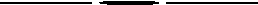
\includegraphics[width=4in]{_Images/poly-filet-colorless.pdf}};
        \node[anchor=center, black] at ($(current page.north) + (1.5in,-2.4in)$) {\resizebox{!}{.25in}{\bfseries\fontfamily{lmr}\version}};
        \node[anchor=center, black] at ($(current page.north) + (1.5in,-2.9in)$) {\resizebox{!}{.2in}{\oldstylenums{\today}, \myauthor}};
        \node[anchor=center, text width=4in, gray, align=justify] at ($(current page.center) + (1.5in, -5in)$) {\itshape Ce document est mis à disposition selon les termes de la licence \href{https://creativecommons.org/licenses/by-nc/4.0/}{Attribution - Utilisation non commerciale 4.0 International}, Olivier Allard 2026.};
    \end{tikzpicture}
\end{titlepage}

\tableofcontents

\clearpage
Ce cours est une copie des cours de \textit{Physique Quantique Avancée} de \textbf{Manuel Joffre}, dispensé à l’École polytechnique, ainsi que du cours de \textit{Mécanique Quantique} de \textbf{Claude Cohen-Tannoudji}.


Il n’a pas de portée pédagogique mais est plutôt pensé comme un ensemble de grands résultats fondamentaux en physique quantique, dans lesquels on peut piocher les informations requises.

\clearpage
\part{Généralités}

\section{Principes fondamentaux}

\subsection{Espace des états}

\begin{omed}{Principe 1}
    À chaque système physique est associé un espace de Hilbert complexe $\mathcal{E}_H$, l’état physique du système étant entièrement défini par un ket normé $\ket{\psi} \in \mathcal{E}_H$.
\end{omed}

    On s’intéresse dans ce cours uniquement à des espaces de Hilbert dits \textit{séparables}, ce qui signifie qu’il admet au moins un ensemble dénombrable de kets $\ket{\psi_n}$ constituant une base orthonormée de l’espace.  

\subsection{Mesure}

On se place premièrement dans le cas \textbf{non-dégénéré}.

\begin{omed}{Principe 2}
    \begin{enumerate}[label=($p_{\arabic*}$)]
        \item À toute grandeur physique $A$ on associe un opérateur linéaire hermitien $\hat{A}$ de $\mathcal{E}_H$ appelé \textbf{observable}. On suppose ici que le spectre de $\hat{A}$ est \textit{discret} et \textit{non-dégénéré}.
        \item Une mesure de $A$ ne peut donner comme résultat qu’une valeur propre $a_n$ de $\hat{A}$.
        \item Pour un système se trouvant dans l’état $\ket{\psi}$, la probabilité de mesurer $a_n$ est
              \[ \mathbb{P}(a_n) := \abs{\spr{\psi_n}{\psi}}^2 \]
              où $\ket{\psi_n}$ est le vecteur propre associé à la valeur propre $a_n$.
        \item Si la mesure de $A$ donne $a_n$, alors le système est dans l’état $\ket{\psi_n}$ après mesure.
    \end{enumerate}
\end{omed}

Dans le cas général,

\begin{omed}{Principe 2}
    \begin{enumerate}[label=($p_{\arabic*}$)]
        \item À toute grandeur physique $A$ on associe un opérateur linéaire hermitien $\hat{A}$ de $\mathcal{E}_H$ appelé \textbf{observable}. On suppose ici que le spectre de $\hat{A}$ est de spectre discret.
        \item Une mesure de $A$ ne peut donner comme résultat qu’une valeur propre $a_n$ de $\hat{A}$.
        \item Pour un système se trouvant dans l’état $\ket{\psi}$, la probabilité de mesurer $a_n$ est
              \[ \mathbb{P}(a_n) := \bra{\psi} \hat{P}_n \ket{\psi} = \nor{\hat{P}_n \ket{\psi}}^2 \]
              où $\hat{P}_n$ est le projecteur sur le sous-espace propre associé à la valeur propre $a_n$.
        \item Si la mesure de $A$ donne $a_n$, alors le système après mesure est dans l’état
              \[ \ket{\psi'} = \frac{\hat{P}_n \ket{\psi}}{\nor{\hat{P}_n \ket{\psi}}} \]
    \end{enumerate}
\end{omed}

\subsection{Évolution temporelle}

\begin{omed}{Principe 3}
    L’évolution de l’état $\ket{\psi(t)}$ du système est gouvernée par l’\textbf{équation de Schrödinger}
    \[ i\hbar \frac{\text{d}\ket{\psi(t)}}{\text{d}t} = \hat{H}(t) \ket{\psi(t)} \]
    où $\bar{H}(t)$ est un observable appelé \textbf{Hamiltonien} et représentant l’énergie du système.
\end{omed}

On peut écrire l’état du système $\ket{\psi(t)}$ à l’instant $t$ à partir de l’état $\ket{\psi(t_0)}$ à l’instant $t_0$ à l’aide d’un opérateur unitaire $\hat{U}(t,t_0)$ appelé opérateur d’évolution selon l’expression 
\[ \ket{\psi(t)} = \hat{U}(t,t_0) \ket{\psi(t_0)} \]   
L’opérateur d’évolution obéit alors à l’équation différentielle 
\[ i\hbar \frac{\partial U(t,t_0)}{\partial t} = \hat{H}(t) \hat{U}(t,t_0) \]   
Dans le cas d’un hamiltonien indépendant du temps, la solution de cette équation s’écrit simplement 
\[ \hat{U}(t,t_0) = \hat{U}(t-t_0) = \exp\left(-i\frac{\hat{H}(t-t_0)}{\hbar}\right) \]  
ce qui donne la solution
\[ \ket{\psi(t)} = \exp\left(-i\frac{\hat{H}}{\hbar}(t - t_0)\right) \ket{\psi(t_0)} \]
\section{Outils mathématiques}

    \subsection{Notation de Dirac}

        On se place dans l’espace des états $\mathcal{E}_H$. 

        On désigne par \textbf{ket} et on note $\ket{\psi}$ tout vecteur de $\mathcal{E}_H$. 

        On désigne par \textbf{bra} et on note $\bra{\phi}$ tout vecteur de $\mathcal{E}_H^*$ qui est l’unique fonctionnelle linéaire (d’après le théorème de représentation de Riesz) associée $\ket{\phi}$. :
        \[ \bra{\phi} : \ket{\psi} \in \mathcal{E}_H \mapsto \spr{\phi}{\psi} \]

        \subsubsection{Opérateurs linéaires}

        Un opérateur linéaire $\hat{A} : \mathcal{E}_H \to \mathcal{E}_H$ est une fonction linéaire de $\mathcal{E}_H$ dans lui-même. 

        Si on considère une base $\left\{\ket{\psi_n}\right\}$ de $\mathcal{E}_H$, on peut définir la matrice de l’opérateur dans cette base, qui aura pour coefficients 
        \[ A_{m,n} = \bra{\psi_m} \hat{A} \ket{\psi_n} \]
        ce qui permet d’écrire directement l’opérateur sous la forme 
        \[ \hat{A} = \sum_{m,n} A_{m,n} \ket{\psi_m} \bra{\psi_n} \]  

        L’opérateur le plus commun est l’identité, qui peut s’écrire dans une base de $\mathcal{E}_H$ comme 
        \[ \hat{I} = \sum_{n} \hat{P}_n := \sum_{n} \ket{\psi_n} \bra{\psi_n} \]   
        où les $\hat{P}_n$ sont les projecteurs sur l’espace $\ket{\psi_n}$, grâce à l’orthonormalité de la base. On appelle cette écriture la \textbf{relation de fermeture}.

        \begin{omed}{Définition}
            Un opérateur $\hat{A}$ est dit \textbf{hermitien} ou \textbf{auto-adjoint} lorsque $\hat{A} = \hat{A}^{\dagger}$ où $\dagger$ est le symbole représentant l’opération de \textit{trans-conjugaison}.
        \end{omed}

        \begin{omed}{Théorème spectral}
            Soit $\hat{A}$ un opérateur hermitien. On suppose que son spectre est \textit{discret}. 

            Alors $\hat{A}$ est diagonalisable : il existe une base orthonormée $\left\{\ket{\psi_n}\right\}$ constituée de vecteurs propres de $\hat{A}$, et 
            \[ \hat{A} = \sum_n a_n \ket{\psi_n} \bra{\psi_n} \]   
        \end{omed}

    \subsection{Transformation de Fourier}

        On sait que l’espace des états $\mathcal{E}_H$ est homéomorphe à $\mathcal{L}^2(\mathbf{R})$ et on se place dans cette sous-section dans le formalisme de $\mathcal{L}^2(\mathbf{R})$. 
        
        On considère la fonction d’onde $\psi(x) = \spr{x}{\psi}$ qui décrit l’état physique du système dans l’\textbf{espace direct} (associé à la position). On cherche l’expression de $\tilde{\psi}(p) = \spr{p}{\psi}$. qui décrit l’état physique du système dans l’\textbf{espace de Fourier} (associé à l’impulsion). 

        \begin{align*}
            \tilde{\psi}(p) &= \spr{p}{\psi} = \bra{p} \hat{I} \ket{\psi} \\
            &= \bra{p} \left(\int \ket{x} \bra{x} dx\right) \ket{\psi} \\
            &= \int \psi(x) \spr{p}{x} dx \\
        \end{align*}
        
        Pour trouver l’expression de $\spr{p}{x} = \overline{\spr{x}{p}}$, considérons l’action de $\hat{p}$ sur une fonction d’onde particulière : l’onde plane $e^{ikx}$, qui est une fonction propre de $\hat{p}$ pour la valeur propre $\hbar k$. Cela implique que 
        \[ \bra{x} \hat{p} \ket{\psi} = \hat{p}\psi(x) = \frac{\hbar}{i} \frac{\text{d}\psi}{\text{d}x} \]
        Ainsi, 
        (trouver pk $\spr{p}{x} = \frac{e^{\frac{- i p x}{\hbar}}}{\sqrt{2\pi \hbar}}$)

        Donc 
        \[ \tilde{\psi}(p) = \frac{1}{\sqrt{2 \pi \hbar}} \int \psi(x) \exp\left(\frac{- i p x}{\hbar}\right) dx := \mathcal{F}[\psi](p) \]
        où $\mathcal{F}$ est la \textbf{transformation de Fourier}, qui nous envoie dans l’espace de Fourier.

        Des calculs similaires nous donnent directement 
        \[ \psi(x) = \frac{1}{\sqrt{2 \pi \hbar}} \int \tilde{\psi}(p) \exp\left(\frac{i p x}{\hbar}\right) := \tilde{\mathcal{F}}[\tilde{\psi}](x) \]   
        où $\tilde{\mathcal{F}}$ est la \textbf{tranformation de Fourier inverse}, qui nous permet de revenir dans l’espace direct.

        \subsubsection{Propriétés}

        \begin{omed}{Théorème}
            Soient deux fonctions d’onde $\psi_1(x)$ et $\psi_2(x)$.
            \[ \int \psi_1^*(x) \psi_2(x) dx = \int \tilde{\psi}_1^*(x) \tilde{\psi}_2(x) dx \]
        \end{omed}

        \begin{demo}{Démonstration}
            Dans le cadre du formalisme de Dirac, on a directement, d’après les relations de fermeture,
            \begin{align*}
                \spr{\psi_1}{\psi_2} &= \int \spr{\psi_1}{x} \spr{x}{\psi_2} dx \\&= \int \spr{\psi_1}{p} \spr{p}{\psi_2} dp
            \end{align*}
        \end{demo}

        \begin{omed}{Proposition}
            Soit $\psi(x)$ une fonction d’onde. 
            \begin{align*}
                \mathcal{F}\left[\frac{\text{d}^n \psi}{\text{d}x^n}\right] &= \left(\frac{ip}{\hbar}\right)^n \mathcal{F}[\psi] \\
                \tilde{\mathcal{F}}\left[\frac{\text{d}^n \tilde{\psi}}{\text{d}p^n}\right] &= \left(-\frac{ix}{\hbar}\right)^n \tilde{\mathcal{F}}[\tilde{\psi}] \\
            \end{align*}
        \end{omed}

        \begin{demo}{Preuve}
            On dérive sous l’intégrale.
        \end{demo}

        \begin{omed}{Proposition}
            Soit $\psi(x)$ une fonction d’onde. 
            \begin{align*}
                \mathcal{F}[\psi(x - x_0)](p) &= \tilde{\psi}(p)\exp\left(-\frac{i p x_0}{\hbar}\right) \\
                \tilde{\mathcal{F}}[\tilde{\psi}(p - p_0)](x) &= \psi(x)\exp\left(\frac{i p_0 x}{\hbar}\right) 
            \end{align*}
        \end{omed}

        \begin{demo}{Preuve}
            Le facteur de phase apparaît dans la tranformation de Fourier de la fonction tranlatée.
        \end{demo}

        \begin{omed}{Proposition}
            Soient deux fonctions d’onde $\psi_1(x)$ et $\psi_2(x)$.
            \begin{align*}
                \mathcal{F}[\psi_1 \psi_2](p) &= \frac{1}{\sqrt{2 \pi \hbar}} (\tilde{\psi_1} \star \tilde{\psi_2}) (p)  \\
                \tilde{\mathcal{F}}[\tilde{\psi}_1 \tilde{\psi}_2](x) &= \frac{1}{\sqrt{2 \pi \hbar}} (\psi_1 \star \psi_2) (p)  \\
            \end{align*}
        \end{omed}


    \subsection{Produit tensoriel}

    Soient $\mathcal{E}_a$ et $\mathcal{E}_b$ deux espaces de Hilbert associés aux sous-systèmes $(a)$ et $(b)$, munis des bases hilbertiennes $\left\{\ket{\alpha_m}\right\}$ et $\left\{ \ket{\beta_n} \right\}$. 

    \begin{omed}{Définition}
        Le \textbf{produit tensoriel} est un opérateur bilinéaire 
        \[ \otimes : \mathcal{E}_a \times \mathcal{E}_b \to \mathcal{E}_a \otimes \mathcal{E}_b \] 
        où $\mathcal{E}_H := \mathcal{E}_a \otimes \mathcal{E}_b$ est un espace vectoriel de Hilbert permettant de décrire l’état du système $\left\{ (a),(b) \right\}$ de base hilbertienne dite \textbf{base tensorielle} $\left\{ \ket{\alpha_m} \otimes \ket{\beta_n} \right\}$.
    \end{omed}

    La base tensorielle nous indique que $\dim(\mathcal{E}_H) = \dim(\mathcal{E}_a) \times \dim(\mathcal{E}_b)$, et la forme générale d’un élément de $\mathcal{E}_H$ est donc 
    \[ \ket{\psi} = \sum_{m,n} c_{m,n} \ket{\alpha_m} \otimes \ket(\beta_m) \] 

    On appellera alors \textbf{états factorisés} les $\ket{\phi} \in \mathcal{E}_H$ qui s’écrivent sous la forme 
    \[ \ket{\phi} = \left( \sum_{m} a_m \ket{\alpha_m} \right) \otimes \left( \sum_{n} b_n \ket{\beta_n} \right) \]
    \textit{i.e.} les états tels que $c_{m,n} = a_m b_n$. On parle dans le cas contraire d’\textbf{état intriqué}. 


    \subsection{Inégalité de Heisenberg}

        Résultat fameux de la physique quantique, stipulant que l’on aura toujours $\Delta x \Delta p \geq \frac{\hbar}{2}$, l’inégalité de Heisenberg peut être démontrée dans un cadre plus général pour deux observables quelconques $\hat{A}$ et $\hat{B}$.

        Commençons dans un premier temps par prouver l’\textbf{inégalité de Cauchy-Schwarz}.

        \begin{omed}{Proposition}
            Soit $\ket{\psi}, \ket{\psi}$ des éléments d’un espace de Hilbert $\mathcal{E}_H$. 
            \[ \abs{\spr{\psi}{\psi'}} \leq \spr{\psi}{\psi} \spr{\psi'}{\psi'} \]
            avec égalité dans le cas où il existe un scalaire $\lambda \in \mathbf{C}$ tel que $\ket{\psi} = \lambda \ket{\psi'}$.
        \end{omed}

        \begin{demo}{Preuve}
            
        \end{demo}

        On considère désormais un système placé dans l’état $\ket{\psi} $ ainsi que . 

        \begin{omed}{Théorème}
            Soient $\ket{\psi} \in \mathcal{E}_H$ et deux observables $\hat{A}$ et $\hat{B}$.
            \[ \Delta A \Delta B \geq \frac{1}{2} \abs{\bra{\psi} \left[\hat{A}, \hat{B}\right] \ket{\psi}} \]
            avec saturation (égalité) lorsque, pour un certain scalaire $\lambda \in \mathbf{R}$, 
            \[ \left(\hat{B} - \left<B\right>\right) \ket{\psi} = i \lambda \left(\hat{A} - \left<A\right>\right) \ket{\psi} \]
        \end{omed}

        \begin{demo}{Démonstration}
            
        \end{demo}

        Dans le cas particulier des observables position $\hat{x}$ et impulsion $\hat{p}$, sachant que leur commutateur est $\left[ \hat{x}, \hat{p} \right] = i \hbar \hat{I}$, on obtient 
        \[ \Delta x \Delta p \geq \frac{\hbar}{2} \]
        
        Le cas de saturation s’obtient lorsque l’on a $\Delta x \Delta p = \frac{\hbar}{2}$. Considérons d’abord le cas particulier d’un paquet d’onde centré $\ket{\psi_0}$ (\textit{i.e.} tel que $\left<x\right> = \left<p\right> = 0$). La saturation impose qu’il existe un nombre réel tel que $\hat{p} \ket{\psi_0} = i \lambda \hat{x} \ket{\psi_0}$ soit, dans l’espace $\mathcal{L}^2(\mathbb{R})$, 
        \[ \frac{\hbar}{i} \frac{\text{d} \psi_0}{\text{d}x}(x) = i \lambda x \psi_0(x) \] 
        Il s’agit de l’équation différentielle génératrice d’une gaussienne, qui admet la solution normalisée 
        \[ \psi_0(x) = \frac{1}{\left(2 \pi \Delta x^2\right)^{\frac{1}{4}}} \exp\left(-\frac{x^2}{4 \Delta x^2}\right) \]  
        
        Ramenons-nous désormais au cas général : on considère $\ket{\psi_1}$ résultant d’une translation dans l’espace de Fourier d’une quantité $p_0$ (\textit{i.e.} $\tilde{\psi}_1(p) = \tilde{\psi}_0(p - p_0)$). Cela revient à une multiplication de phase dans l’espace direct : 
        \[ \psi_1(x) = \psi_0(x) \exp\left(\frac{i p_0 x}{\hbar}\right) \]   
        On effectue ensuite une translation dans l’espace direct pour obtenir un état centré sur une posittion $x_0$ arbitraire. Finalement, 
        \[ \psi(x) = \frac{e^{\frac{i p_0 (x - x_0)}{\hbar}}}{\left(2 \pi \Delta x^2\right)^{\frac{1}{4}}} \exp\left(-\frac{(x - x_0)^2}{4 \Delta x^2}\right) \]

        Dans l’espace de Fourier, cette gaussienne prend la forme 
        \begin{align*}
            \tilde{\psi}(p) &= \frac{e^{-\frac{i p x_0}{\hbar}}}{\left(\frac{\pi \hbar^2}{2 \Delta x^2}\right)^{\frac{1}{4}}} \exp\left(-\frac{(p - p_0)^2}{\frac{\hbar^2}{\Delta x^2}}\right) \\
            &= \frac{e^{-\frac{i p x_0}{\hbar}}}{\left(2 \pi \Delta p^2\right)^{\frac{1}{4}}} \exp\left(-\frac{(p - p_0)^2}{4 \Delta p^2}\right)
        \end{align*}

\section{Oscillateur harmonique en physique quantique}

    \subsection{Oscillateur harmonique classique}

        \subsubsection{Cas général}

        On considère une particule dans un puits de potentiel de la forme $V(x) = \frac{1}{2} kx^2$. D’après le principe fondamental de la dynamique, 
        \[ m \frac{\text{d}^2 x}{\text{d}t^2} = - \frac{\text{d}V}{\text{d}x} = - kx \]   
        Cette équation admet les solutions de la forme $x = x_M \cos(\omega t - \varphi)$ où $\omega = \sqrt{\frac{k}{m}}$ et les constantes d’intégration $x_M$ et $\varphi$ dépendent des conditions initiales. L’énergie de la particule est alors 
        \begin{align*}
            E 
            &= T + V \\
            &= \frac{p^2}{2m} + \frac{1}{2} m \omega^2 x^2 \\
            &= \frac{1}{2} m \omega^2 x_M^2
        \end{align*} 
        Il est notable que l’énergie de la particule dans ce puits de potentiel soit indépendante du temps.

        \subsubsection{Mouvement autour d’une position d’équilibre}

        On considère un potentiel $V(x)$ quelconque présentant un mimimum en $x = x_0$ :
        \begin{align*}
            V(x) 
            &= V(x_0) + \frac{1}{2} \left(\frac{\text{d}^2 V}{\text{d}x^2}\right)_{x = x_0}(x - x_0)^2 + o_{x \to x_0} \left((x - x_0)^2\right) \\
            &:= a + b (x - x_0)^2 + o_{x \to x_0} \left((x - x_0)^2\right) \\
        \end{align*}
        Le point $x = x_0$ correspond à une position d’équilibre stable pour la particule puisque $F_x$ est nulle pour $x = x_0$ et de signe opposé à $x-x_0$ sinon. Pour un mouvement d’amplitude suffisamment petite pour que le terme en $(x - x_0)^3$ soit négligeable, on a alors affaire à un oscillateur harmonique puisque le principe de la dynamique s’écrit 
        \[ m \frac{\text{d}^2 x}{\text{d}t^2} \approx -2b(x-x_0) \]   
        La pulsation associée à cet oscillateur harmonique est alors 
        \[ \omega = \sqrt{\frac{1}{m} \left(\frac{\text{d}^2 V}{\text{d}x^2}\right)_{x = x_0}}  \]

    \subsection{Oscillateur harmonique quantique}

        Plaçons nous désormais dans le cadre de la mécanique quantique, avec $V(\hat{x}) = \frac{1}{2} m \omega^2 \hat{x}^2$. L’hamiltonien s’écrit alors 
        \[ \hat{H} = \frac{\hat{p}^2}{2m} + \frac{1}{2} m \omega^2 \hat{x}^2 \]   
        et l’équation aux valeurs propres associée 
        \[\left( - \frac{\hbar^2}{2m} \frac{\text{d}^2}{\text{d}x^2} + \frac{1}{2} m \omega^2 x^2  \right) \varphi(x) = E \varphi(x) \]
        On remarque que $E \geq 0$, et que le puits de potentiel étant symétrique, les fonctions d’onde solutions sont nécessairement de parité définie.

        \subsubsection{Les opérateurs $\hat{X}$, $\hat{P}$, $\hat{a}$ et $\hat{N}$}

        Cherchons à nous ramener à des grandeurs sans dimension, en posant 
        \begin{align*}
            \hat{X} &= \sqrt{\frac{m\omega}{\hbar}}X \\
            \hat{P} &= \frac{1}{\sqrt{m\hbar\omega}}P
        \end{align*}
        L’hamiltonien peut alors s’écrire 
        \[ \hat{H} = \frac{\hbar\omega }{2}\left(\hat{X}^2 + \hat{P}^2\right) \]   
        On pose ensuite les opérateurs
        \begin{align*}
            \hat{a} &= \frac{1}{\sqrt{2}}\left(\hat{X} + i \hat{P}\right) \\
            \hat{a}^{\dagger} &= \frac{1}{\sqrt{2}}\left(\hat{X} - i \hat{P}\right) \\
        \end{align*}
        qui permettent de réécrire les opérateurs $\hat{X} = \frac{1}{\sqrt{2}}(a^{\dagger} + \hat{a})$ et $\hat{P}= \frac{1}{\sqrt{2}}(a^{\dagger} - \hat{a})$, ainsi que l’hamiltonien 
        \begin{align*}
            \hat{H} 
            &= \hbar \omega \left(\frac{1}{2} +  a^{\dagger} \hat{a}\right) \\
            &:= \hbar \omega \left(\frac{1}{2} + \hat{N}\right)
        \end{align*}
        La recherche des vecteurs propres de $\hat{H}$ se fait donc à travers celle de $\hat{N}$. Calculons les commutateurs utiles pour cette étude :
        \begin{align*}
            \left[a, a^{\dagger}\right] 
            &= \frac{i}{2} \left[\hat{P}, \hat{X}\right] - \frac{i}{2} \left[\hat{X}, \hat{P}\right]  \\
            &= 1 \\
            \left[\hat{N}, \hat{a}\right] 
            &= \hat{a}^{\dagger} \left[\hat{a}, \hat{a}\right] + \left[a^{\dagger}, \hat{a} \right] \hat{a} \\
            &= - \hat{a} \\
            \left[\hat{N}, \hat{a}^{\dagger}\right] 
            &= \hat{a}^{\dagger} \left[\hat{a}, \hat{a}^{\dagger}\right] + \left[a^{\dagger}, \hat{a}^{\dagger}\right] \hat{a} \\
            &= \hat{a}^{\dagger} \\
        \end{align*}

        \subsubsection{Spectre de $\hat{N}$ et de $\hat{H}$}

        Les valeurs propres de $\hat{N}$ sont dans $\mathbf{R}_+$ car pour tout vecteur propre $\ket{\psi_{n}}$ de $\hat{N}$, 
        \[ \nor{\hat{a} \ket{\psi_n}}^2 = E_n \geq 0 \]
        Considérons maintenant l’effet de $\hat{a}$ et $\hat{a}^{\dagger}$ sur un vecteur propre de $\hat{N}$ $\ket{\psi_n}$. D’après les relation de commutation,
        \begin{align*}
            \hat{N} \hat{a}\ket{\psi_n} 
            &= \hat{a} \hat{N} \ket{\psi_n} - \hat{a} \ket{\psi_n} \\
            &= (E_n - 1) \hat{a}\ket{\psi_n} \\
            \hat{N} \hat{a}^{\dagger}\ket{\psi_n} 
            &= \hat{a}^{\dagger} \hat{N} \ket{\psi_n} + \hat{a}^{\dagger} \ket{\psi_n} \\
            &= (E_n + 1) \hat{a}^{\dagger} \ket{\psi_n} \\
        \end{align*}
        On appelle $\hat{a}$ l’\textbf{opérateur annihilation} et $\hat{a}^{\dagger}$ l’\textbf{opérateur création}, dont les actions respectives font descendre ou grimper d’une unité dans les valeurs propres de $\hat{N}$. Il est impossible qu’un vecteur propre soit associée à une énergie non-entière, auquel cas les applications successives de $\hat{a}$ nous fournirait à terme une énergie $E < 0$. Ainsi, tout énergie associée à $\hat{N}$ est entière. Par applications de $\hat{a}$ ou $\hat{a}^{\dagger}$, on peut donc obtenir n’importe quelle valeur d’énergie dans $\mathbf{N}$ : 
        \[ \text{Sp}(\hat{N}) = \mathbf{N} \]
        Les valeurs propres de l’hamiltonien seront alors de la forme 
        \[ E_n = \hbar \omega \left(n + \frac{1}{2}\right) \]
        En mécanique quantique, l’énergie de l’oscillateur harmonique est \textit{quantifiée}.


        
\section{Méthodes d’approximation}

    Seuls certains problèmes de mécanique quantique (oscillateur harmonique, mouvement d’une particule chargée dans un potentiel coulombien) peuvent être résolus de façon exacte. Pour d’autres problèmes, on se ramène à des méthodes d’appoximation.

    \subsection{Méthode des perturbations}

        \subsubsection{Principe}

    Cette méthode repose sur la recherche des valeurs et vecteurs propres d’un hamiltonien indépendant du temps, sachant que celui-ci peut s’écrire sous la forme $\hat{H} = \hat{H}_0 + \hat{W}$, où $\hat{H}_0$ représente l’hamiltonien principal tandis que $\hat{W}$ est une perturbation supposée petite devant $\hat{H}_0$. 

    On suppose que les vecteurs et valeurs propres de $\hat{H}_0$ sont connues, et on notera 
    \[ \hat{H}_0 \ket{n,r} = E_n \ket{n,r} \]   
    où $r \in \intEN{1}{g_n}$ représente le niveau de dégénérescence du niveau d’énergie $E_n$. On posera $\hat{W} = \lambda \hat{H}_1$ où $\hat{H}_1$ est du même ordre de grandeur que $\hat{H}_0$ tandis que $\lambda \ll 1$. 

    L’idée de base de la méthode constiste à considérer les vecteurs propres $\ket{\psi(\lambda)}$ et ses valeurs propres $E(\lambda)$ de l’hamiltonien $\hat{H}(\lambda) = \hat{H}_0 + \lambda \hat{H}_1$ et à effectuer un développement limité en fonction de $\lambda$ lorsque $\lambda \to 0$. On a ainsi 
    \[ \ket{\psi(\lambda)} = \ket{\psi^{(0)}} + \lambda \ket{\psi^{(1)}} + \cdots \] 
    et 
    \[ E(\lambda) = E^{(0)} + \lambda E^{(1)} + \cdots \]   
    L’équation aux valeurs propres s’écrit alors 
    \begin{align*}
        \left(\hat{H}_0 + \lambda \hat{H}_1\right) \ket{\psi(\lambda)} &= E(\lambda) \ket{\psi(\lambda)} 
        \left(\hat{H}_0 + \lambda \hat{H}_1 \right)\left(\ket{\psi^{(0)}} + \lambda \ket{\psi^{(1)}} + \cdots\right) = \left(E^{(0)} + \lambda E^{(1)} + \cdots\right)\left(\right)\left(\ket{\psi^{(0)}} + \lambda \ket{\psi^{(1)}} + \cdots\right)
    \end{align*}
    En identifiant les coefficients d’ordre successifs dans les polynômes en $\lambda$ figurant dans les deux membres de l’égalité ci-dessus, on obtient donc que 
    \begin{align*}
        \hat{H}_0 \ket{\psi^{(0)}} &= E^{(0)} \ket{\psi^{(0)}} \\
        \hat{H}_0 \ket{\psi^{(1)}} + \hat{H}_1 \ket{\psi^{(0)}} &= E^{(0)} \ket{\psi^{(1)}} + E^{(1)} \ket{\psi^{(0)}} \\  
        &\vdots
    \end{align*}
    
    La méthode consiste à résoudre successivement cette hiérarchie d’équations, en allant jusqu’à l’ordre d’approximation souhaité. On va ici se restreindre au second ordre, souvent largement suffisant.

        \subsubsection{Cas d’un niveau non dégénéré}

    On considère le cas où $E^{(0)}$ est non dégénéré. On pose $E^{(0)} = E_n$ et $\ket{\psi^{(0)}} = \ket{n}$ où $E_n$ est l’une des valeurs propres de $\hat{H}_0$. On a alors le système d’équations (en se limitant au premier ordre) 
    \begin{align*}
        \hat{H}_0 \ket{n} &= E_n \ket{n} \\
        \hat{H}_0 \ket{\psi^{(1)}} + \hat{H}_1 \ket{n} &= E_n \ket{\psi^{(1)}} + E^{(1)} \ket{n}
    \end{align*}
    En multipliant à gauche la deuxième équation par le bra $\bra{m}$, vecteur propre de $\hat{H}_0$ pour la valeur propre $E_m$, on obtient 
    \begin{align*}
        \bra{m} \hat{H}_0 \ket{\psi^{(1)}} + \bra{m} \hat{H}_1 \ket{n} &= E_n \spr{m}{\psi^{(1)}} + E^{(1)} \spr{m}{n} \\
        \bra{m} \hat{H}_1 \ket{n} &= (E_n - E_m) \spr{m}{\psi^{(1)}} + E^{(1)} \spr{m}{n}
    \end{align*}
    En appliquant ce résultat au cas $m = n$, on obtient que 
    \[ E^{(1)} = \bra{n} \hat{H}_1 \ket{n} \]   
    Puis avec $m \neq n$, on obtient que 
    \[ \spr{m}{\psi^{(1)}} = \frac{\bra{m} \hat{H}_1 \ket{n}}{E_n - E_m} \] 
    Cette équation nous informe sur la valeur de $\spr{m}{\psi^{(1)}}$ pour tout $m \neq n$ mais ne nous donne pas d’information sur $\spr{n}{\psi^{(1)}}$. On peut déterminer sa valeur par un développement de $\ket{\psi(\lambda)}$ au premier ordre en $\lambda$ :
    \begin{align*}
        \spr{\psi(\lambda)}{\psi(\lambda)}
        &= \left(\bra{n} + \lambda \bra{\psi^{(1)}}\right) \left(\ket{n} + \lambda \ket{\psi^{(1)}}\right) + O_{\lambda \to 0} \left(\lambda^2\right) \\
        &= 1 + \lambda \left(\spr{n}{\psi^{(1)}} + \spr{\psi^{(1)}}{n}\right) + O_{\lambda \to 0} \left(\lambda^2\right)
    \end{align*}
    La condition de normalisation du ket $\ket{\psi(\lambda)}$ implique que la partie réelle de $\spr{n}{\psi^{(1)}}$ soit nulle et donc $\spr{n}{\psi^{(1)}} = i \beta$. Ainsi, 
    \begin{align*}
        \ket{\psi^{(1)}}
        &= \sum_{m} \ket{m} \spr{m}{\psi^{(1)}} \\
        &= \ket{n}\spr{n}{\psi^{(1)}} + \sum_{m \neq n} \ket{m} \spr{m}{\psi^{(1)}} \\
        &= i \beta \ket{n} + \sum_{m \neq n} \frac{\bra{m} \hat{H}_1 \ket{n}}{E_n - E_m} \ket{m}
    \end{align*} 
    Le paramètre $\beta$ est libre, et peut prendre n’importe quelle valeur. Il est lié à la phase globale du vecteur d’état :
    \begin{align*}
        \ket{\psi(\lambda)} 
        &= \ket{\psi^{(0)}} + \ket{\psi^{(1)}} + O_{\lambda \to 0} \left(\lambda^2\right) \\
        &= \left(1 + i \lambda \beta\right) \ket{n} + \lambda \sum_{m \neq n} \frac{\bra{m} \hat{H}_1 \ket{n}}{E_n - E_m} \ket{m} + O_{\lambda \to 0} \left(\lambda^2\right) \\
        &= e^{i \lambda \beta} \left(\ket{n} + \lambda \sum_{m \neq n} \frac{\bra{m} \hat{H}_1 \ket{n}}{E_n - E_m} \ket{m} \right) + O_{\lambda \to 0} \left(\lambda^2\right)
    \end{align*}
    La phase n’ayant pas d’impact sur l’état, on peut choisir $\beta = 0$, ce qui donne finalement 
    \[ \ket{\psi^{(1)}} = \sum_{m \neq n} \frac{\bra{m} \hat{H}_1 \ket{n}}{E_n - E_m} \ket{m} \]   
    Pour l’ordre 2, considérons la troisième équation provenant de l’égalité initiale $\hat{H}_{\lambda} \ket{\psi(\lambda)} = E(\lambda) \ket{\psi(\lambda)}$, 
    \[ \hat{H}_0 \ket{\psi^{(2)}} + \hat{H}_1 \ket{\psi^{(1)}} =  E^{(0)} \ket{\psi^{(2)}} + E^{(1)} \ket{\psi^{(1)}} + E^{(2)} \ket{\psi^{(0)}} \]    
    et projetons-la sur le bra $\bra{n}$. Comme $\bra{n}\hat{H}_0 = E_n \bra{n}$ et $\spr{n}{\psi^{(1)}} = 0$, on obtient que 
    \[ E^{(2)} = \bra{n} \hat{H}_1 \ket{\psi^{(1)}} = \sum_{m \neq n} \frac{\abs{\bra{m} \hat{H}_1 \ket{n}}^2}{E_n - E_m} \]   

    \begin{omed}{Méthode des perturbations (cas non dégénéré)}
        On considère un hamiltonien $\hat{H}_0$ (d’états propres $\left\{\ket{n}\right\}$ connus et non dégénérés tels que $\hat{H}_0 \ket{n} = E_n \ket{n}$) auquel on ajoute une perturbation $\hat{W}$ petite devant $\hat{H}_0$. On peut écrire l’énergie sous la forme du développement 
        \[ E = E_n + \delta E_n^{(1)} + \delta E_n^{(2)} + \cdots \]   
        où $\delta E_n^{(k)}$ correspond au terme d’ordre $k$ en $\hat{W}$. On obtient alors les expressions suivantes du déplacement de l’énergie au premier et second ordre :
        \begin{align*}
            \delta E_n^{(1)} &= \bra{n} \hat{W} \ket{n} \\
            \delta E_n^{(2)} &= \sum_{m \neq n} \frac{\abs{\bra{m} \hat{W} \ket{n}}^2}{E_n - E_m}
        \end{align*}
        On peut aussi développer l’état propre perturbé de $\hat{H}$ sous la forme 
        \[ \ket{\psi} = \ket{n} + \ket{\delta \psi_n^{(1)}} + \ket{\delta \psi_n^{(2)}} + \cdots \]   
        avec, au premier ordre, 
        \[ \ket{\delta \psi_n^{(1)}} = \sum_{m \neq n} \frac{\bra{m} \hat{W} \ket{n}}{E_n - E_m} \ket{m} \]
    \end{omed}

    Remarquons qu’avec le résultat de cette méthode, on peut interpréter l’énergie au premier ordre par la formule 
    \[ E \equiv E_n + \delta E_n^{(1)} = \bra{n} \hat{H}_0 \ket{n} + \bra{n} \hat{W} \ket{n} = \bra{n} \hat{H} \ket{n} \]   
    L’énergie perturbée d’un niveau donné est donc à peu près égale à la valeur moyenne de l’hamiltonien total dans l’état non perturbé, ce qui constitue un résultat relativement intuitif.

        \subsubsection{Cas d’un niveau dégénéré}

    On considère le cas où $E^{(0)} = E_n$ est dégénéré. On posera ainsi $\hat{H}_0 \ket{n,r} = E_n \ket{n,r}$ où $r \in \intEN{1}{g_n}$ où $g_n$ est la dimension du sous-espace propre associé. Reprenons alors l’étude du système d’équations 
    \begin{align*}
        \hat{H}_0 \ket{\psi^{(0)}} &= E^{(0)} \ket{\psi^{(0)}} \\
        \hat{H}_0 \ket{\psi^{(1)}} + \hat{H}_1 \ket{\psi^{(0)}} &= E^{(0)} \ket{\psi^{(1)}} + E^{(1)} \ket{\psi^{(0)}} \\  
        \hat{H}_0 \ket{\psi^{(2)}} + \hat{H}_1 \ket{\psi^{(1)}} &=  E^{(0)} \ket{\psi^{(2)}} + E^{(1)} \ket{\psi^{(1)}} + E^{(2)} \ket{\psi^{(0)}}  
    \end{align*}
    On peut écrire le vecteur $\ket{\psi^{(0)}}$ comme un élément du sous-espace propre soit 
    \[ \ket{\psi^{(0)}} = \sum_{r=1}^{g_n} c_r \ket{n,r} \]   
    En projetant la seconde équation sur le bra $\bra{n,r}$, sachant que $\bra{n,r} \hat{H}_0 = E_n \bra{n,r}$, on obtient 
    \[ \bra{n,r} \hat{H}_1 \sum_{r' = 1}^{g_n} c_{r'} \ket{n, r'} = E^{(1)} c_r \]   
    qui, après multiplication par $\lambda$ se réécrit 
    \[ \sum_{r'=1}^{g_n} \bra{n,r} \hat{W} \ket{n,r'}c_{r'} = \delta E^{(1)} c_r \]   
    On a alors un système de $g_n$ équations linéaires pouvant s’écrire sous forme matricielle
    \[ \begin{bmatrix}
        \bra{n,1} \hat{W} \ket{n,1} & \cdots & \bra{n,1} \hat{W} \ket{n,g_n} \\
        \vdots & \ddots & \vdots \\
        \bra{n,g_n} \hat{W} \ket{n,1} & \cdots & \bra{n,g_n} \hat{W} \ket{n,g_n} \\
    \end{bmatrix} 
    \begin{bmatrix}
        c_1 \\
        \vdots \\
        c_n
    \end{bmatrix} = \delta E^{(1)} \begin{bmatrix}
        c_1 \\
        \vdots \\
        c_n
    \end{bmatrix} \]    




    \subsection{Méthode variationnelle}

        \subsubsection{Majoration de l’énergie du niveau fondamental}

    Pour tout état $\ket{\psi}$ de l’espace de Hilbert considéré, 
    \[ \bra{\psi} \hat{H} \ket{\psi} \geq E_0 \]   
    où $E_0$ est l’énergie du niveau fondamental. Il y a égalité uniquement lorsque l’état $\ket{\psi}$ appartient au sous-espace propre du niveau fondamental. 

        \subsubsection{La méthode variationnelle}

    Le problème d’optimisation consistant à minimiser la grandeur $\bra{\psi} \hat{H} \ket{\psi}$ est équivalent à la recherche de l’énergie $E_0$ du niveau fondamental et de l’état propre associé. 

    \begin{omed}{Méthode variationnelle}
        La méthode variationnelle consiste à se donner un ensemble $\left\{\ket{\phi_{\alpha}}\right\}$ de vecteurs d’essai appartenant à un sous-ensemble de l’espace de Hilbert et chercher le minimum de la grandeur 
        \[ E(\alpha) = \frac{\bra{\varphi_{\alpha}} \hat{H} \ket{\varphi_{\alpha}} }{\spr{\varphi_{\alpha}}{\varphi_{\alpha}}} \]   
        On approximera ainsi $E_0$ par $E(\alpha_{\text{min}})$ et l’état propre fondamental par $\frac{\ket{\varphi_{\text{min}}}}{\nor{\varphi_{\text{min}}}}$. 
    \end{omed}

    La précision de la méthode dépend de la pertinence de l’espace des fonctions d’essais, souvent choisi par considérations physiques.

        \subsubsection{La méthode variationnelle linéaire}

    Le problème variationnel linéaire correspond au cas particulier où $\mathcal{E}_{\text{essai}}$ est un sous-espace vectoriel de l’espace de Hilbert. 

    \begin{omed}{Méthode variationnelle linéaire}
        La méthode variationnelle linéaire consiste à rechercher les extremums de la fonctionnelle 
        \[ E(\ket{\psi}) = \frac{\bra{\psi} \hat{H} \ket{\psi} }{\spr{\psi}{\psi}} \]   
        où $\ket{\psi} \in \mathcal{E}_{\text{essai}}$ qui est un sous-espace vectoriel de l’espace de Hilbert. Cette recherche s’effectue en diagonalisant la restriction de l’hamiltonien dans l’espace $\mathcal{E}_{\text{essai}}$. Les vecteurs propres et valeurs propres ainsi obtenus constituent des approximations des premiers vecteurs propres et valeurs propres de l’hamiltonien $\hat{H}$. De plus, les valeurs propres obtenues constituent des bornes supérieures des valeurs exactes.
    \end{omed}
 
\section{Symétries en physique quantique}

    \subsection{Invariance et commutation}

        \subsubsection{Le groupe de symétrie}

    On considère le groupe des isométries de l’espace euclidien à trois dimensions (\textit{i.e.} des transformations conservant le produit scalaire donc les distances et les angles) duquel on ne conserve seulement celles \textit{laissant le système physique invariant}. On a ainsi un groupe dit \textbf{groupe de symétrie}, qui peut être discret (rotations $n \times \frac{2\pi}{6}$ du benzène, translations d’un cristal) ou infini (translations d’un système homogène, rotations pour un système invariant par rotation).

    \begin{omed}{Théorème (de Noether)}
        À toute invariance du système on peut associer une quantité physique conservée.
    \end{omed}

    Étudier les symétries d’un système physique est donc judicieux pour trouver des grandeurs conservées.

    Il est intéressant de remarquer que pour toute isométrie d’un espace de Hilbert $\mathcal{E}_H$, la contrainte $\spr{\psi_1}{\psi_2} = \bra{\psi_1} \hat{R}^{\dagger} \hat{R} \ket{\psi_2}$ pour toutes fonctions d’ondes $\ket{\psi_1}, \ket{\psi_2} \in \mathcal{E}_H$ implique que 
    \[  \hat{R}^{\dagger} \hat{R} = \hat{I} \]
    Et étant donné qu’une isométrie est nécessairement inversible, on a directement 
    \[  \hat{R} \hat{R}^{\dagger} = \hat{I} \]
    donc $\hat{R}$ est un \textit{opérateur unitaire}.

        \subsubsection{Commutation avec Ĥ}

    De façon générale, pour tout système invariant par une isométrie $\mathcal{R}$, l’hamiltonien $\hat{H}$ commute avec l’opérateur $\hat{R}$ représentant cette isométrie dans l’espace de Hilbert.

    En effet, considérons un système dans l’état $\ket{\psi(t_0)}$ à un instant initial $t_0$. À $t_1$, ce système aura pour état $\ket{\psi(t_1)} = \hat{U}(t_1, t_0)\ket{\psi(t_0)} $. Que l’on tranforme ce système avant ou après son évolution n’a pas d’impact par définition de l’invariance par l’isométrie. Ainsi, 
    \[ \hat{R}\hat{U}(t_1,t_0)\ket{\psi(t_0)} = \hat{U}(t_1,t_0)\hat{R}\ket{\psi(t_0)} \]
    Par validité pour tout état initial, on a donc 
    \[ \hat{R}\hat{U}(t_1,t_0) = \hat{U}(t_1,t_0)\hat{R} \quad \text{i.e.} \quad \left[\hat{R},\hat{U}(t_1,t_0)\right] = 0 \]
    puis en dérivant par rapport à $t_1$, et sachant que d’après l’équation de Schrödinger $i\hbar\frac{\partial \hat{U}(t,t_0)}{\partial t} = \hat{H}(t)\hat{U}(t,t_0)$, on obtient alors que 
    \[ \left[\hat{R},\hat{H}(t)\right] = 0 \]
    Ceci implique immédiatemment, d’après le théorème d’Erhenfest, que la grandeur $R$ se conserve au cours du temps. 

    Lorsque l’hamiltonien est indépendant du temps, la recherche de ses états propres sera en outre simplifiée par le fait que les opérateurs $\hat{R}$ et $\hat{H}$ peuvent être diagonalisés dans une même base.

        \subsubsection{Générateur infinitésimal}

    On considère un groupe de symétrie continue, que l’on admettra qu’il peut être caractérisé par un paramètre $a$. On admet aussi que lorsque c’est un groupe de Lie, on peut différencier l’opérateur $\mathcal{R}_a$ par rapport à $a$. On appelle \textbf{générateur infinitésimal} l’opérateur $\hat{G}$ défini par 
    \[ \hat{R}_{da} = \hat{I} - \frac{i}{\hbar} \hat{G}da \]   
    Pour satisfaire l’unitarité de $\hat{R}_{da}$, il faut et il suffit que $\hat{G} = \hat{G}^{\dagger}$, \textit{i.e.} que $\hat{G}$ soit un opérateur \textit{auto-adjoint}. On peut donc lui associer une grandeur physique observable. Par définition de $\hat{G}$, on a 
    \[ \hat{G} = i\hbar \frac{\partial \hat{R}_a}{\partial a} (a = 0) \]   
    et sachant que $\left[\hat{R}_{da},\hat{H}(t)\right] = 0$, on trouve que 
    \[ \left[\hat{G}, \hat{H}\right] = 0 \]
    La grandeur physique $G$ associée à $\hat{G}$ est donc une constante du mouvement : il s’agit de la version quantique du théorème de Noether.

    \section{Parité}

    On note $\hat{\Pi}$ l’opérateur parité, dont l’action sur une fonction d’onde est, par exemple sur une fonction d’onde $\psi(x)$ de $\mathcal{L}^2(\mathbf{R})$,
    \[ \left(\hat{\Pi_x}\psi\right)(x) = \psi(-x) \quad \text{i.e.} \quad \bra{x} \hat{\Pi_x} \ket{\psi} = \spr{-x}{\psi} \]
    On a ainsi $\bra{x} \hat{\Pi_x} = \bra{-x}$ et donc, par unitarité $\hat{\Pi_x} \ket{x} = \ket{-x}$, ce que l’on aurait pu prendre comme point de départ.

    On peut aussi considéré l’opérateur parité dans $\mathcal{L}^2(\mathbf{R}^3)$, soit par la symétrie miroir par rapport à $x = 0$ définie par 
    \[ (\hat{\Pi_x}\psi)(x,y,z) = \psi(-x,y,z) \]    
    ou l’inversion définie par 
    \[ (\hat{\Pi}\psi)(\vec{r}) = \psi(-\vec{r}) \quad \text{i.e.} \quad \hat{\Pi}\ket{\vec{r}} = \ket{-\vec{r}} \] 

    On remarque immédiatemment que $\hat{\Pi}^2 = \hat{I}$, donc les valeurs propres de l’opérateur parité sont $\pm 1$. Les états propres associés à la valeur propre $+1$ sont appelés états symétriques ou pairs, et obéissent à la relation $\psi_S(-x) = \psi_S(x)$, et les états associés à $-1$, appelés états antisymétriques ou impairs, obéissent à la relation $\psi_A(-x) = - \psi_A(x)$.

    On peut donc chercher les états propres sous forme d’états pairs et impairs, puis diagonaliser l’hamiltonien dans cette base (étant donné que $\left[\hat{\Pi}_x, \hat{H}\right]$).

    \subsection{Translations}

    Considérons un système inviariant par \textit{toute transformation}, quelle que soit la direction où l’amplitude de la translation considérée. Un tel système est donc nécessairement homogène. 

        \subsubsection{Translation dans L2R}

    On considère les translations de la forme $x \mapsto x + a$, \textit{i.e.} les opérateurs de la forme 
    \[ \hat{T}_a \ket{x} = \ket{x + a} \]    
    Son opérateur adjoint $\hat{T}_a^{\dagger}$ est la translation inverse $\hat{T}_{-a}$. 

    En passant à l’adjoint dans l’égalité, $\hat{T}^{\dagger}_{a}\ket{x} = \ket{x-a}$, on obtient que $\bra{x} \hat{T}_a = \bra{x-a}$ d’où 
    \[ \bra{x} \hat{T}_a \ket{\psi} = \spr{x-a}{\psi} = \psi(x-a) \] 
    
    On peut considérer la translation infinitésimale $\hat{T}_{da}$. On a dans ce cas 
    \begin{align*}
        \bra{x} \hat{T}_{da} \ket{\psi} 
        &= \psi(x - da) \\
        &= \psi(x) - da \frac{\partial \psi}{\partial x} \\
        &= \left(1 - \frac{i}{\hbar}da \frac{\hbar}{i}\frac{\partial }{\partial x} \right) \psi(x) \\
        &= \bra{x} \left(\hat{I} - \frac{i}{\hbar} da \hat{p}_x \right) \ket{\psi}
    \end{align*}

    On en déduit que $\hat{T}_{da} = \hat{I} - \frac{i}{\hbar} da \hat{p}_x$, et que l’impulsion $\hat{p}_x$ est le générateur infinitésimal du groupe des translations. En utilisant l’additivité des opérateurs translations ($\hat{T_{a+b}} = \hat{T_a}\hat{T_b}$), on remarque que 
    \begin{align*}
        \hat{T}_{a + da} 
        &= \hat{T_{da}}\hat{T_a} \\
        &= \hat{T_a} - \frac{i}{\hbar}\hat{p}_x \hat{T_a}da
    \end{align*}
    c’est-à-dire que 
    \[ \frac{\text{d}\hat{T}_a}{\text{d}a} = - \frac{i}{\hbar} \hat{p}_x \hat{T}_a  \]
    On obtient une équation analogue à cette qui porte sur l’opérateur d’évolution, et la solution sera donc de la même forme :
    \[ \hat{T}_a = \exp\left(-\frac{i \hat{p}_x a}{\hbar}\right) \]  
    
        \subsubsection{Translation dans L2R3}

    On généralise la procédure précédente en prenant un vecteur $\vec{a}$, et la translation $T_{\vec{a}}$ s’écrit comme composition des translations selon les trois axes.
    \[ \hat{T}_{\vec{a}} = \exp\left(-\frac{i \hat{p}_z a_z}{\hbar}\right)\exp\left(-\frac{i \hat{p}_y a_y}{\hbar}\right)\exp\left(-\frac{i \hat{p}_x a_x}{\hbar}\right) \]
    par translations entre les opérateurs, on obtient 
    \[ \hat{T}_{\vec{a}} = \exp\left(-\frac{i\hat{\vec{p}}\cdot \vec{a}}{\hbar}\right) \]   
    Si on redéveloppe au plus bas ordre dans le cas d’une transformation infinitésimale, on obtient que 
    \[ \hat{T}_{d\vec{a}} = \hat{I} - \frac{i}{\hbar} \hat{p}_x da_x - \frac{i}{\hbar} \hat{p}_y da_y - \frac{i}{\hbar} \hat{p}_z da_z \]   
    Les observables $\hat{p}_{x,y,z}$ sont donc les générateurs infinitésimaux du groupe des translations.

        \subsbsection{Nouvelle définition de l’observable impulsion}

    Une nouvelle approche basée sur la définition de l’impulsion $\hat{\vec{p}}$ est plus générale puisqu’elle s’applique à tout système physique.

    \begin{omed}{Définition (observable impulsion)}
        On appelle observable impulsion $\hat{\vec{p}}$ l’ensemble des trois opérateurs $(\hat{p}_x, \hat{p}_y, \hat{p}_z)$ définis comme les générateurs infinitésimaux du groupe des translations, de sorte qu’une translation infinitésimale soit représentée dans l’espace de Hilbert par l’opérateur 
        \[ \hat{T}_{d\vec{a}} = \hat{I} - \frac{i}{\hbar} \hat{p}_x da_x - \frac{i}{\hbar} \hat{p}_y da_y - \frac{i}{\hbar} \hat{p}_z da_z \]   
    \end{omed}

    Le groupe des translations étant commutatif, on en déduit que les observables $\hat{p}_x, \hat{p}_y, \hat{p}_z$ commutent entre elles. Dans le cas particulier où $\mathcal{E}_H = \mathcal{L}^2(\mathbf{R}^3)$, on peut chercher l’expression explicite de l’opérateur impulsion à partir de cette nouvelle définition sachant que 
    \begin{align*}
        \bra{\vec{r}} \hat{T}_{d\vec{a}} \ket{\psi} 
        &= \psi(\vec{r} - d\vec{a}) \\
        &= \psi(\vec{r}) - \vec{\nabla}\psi \cdot d\vec{a} \\
        &= \psi(\vec{r}) - \frac{i}{\hbar} \frac{\hbar}{i} \vec{\nabla}\psi \cdot d\vec{a}
    \end{align*}
    ce qui nous donne bien la définition connue dans $\mathcal{L}^2(\mathbf{R}^3)$ 
    \[ \hat{\vec{p}} = \frac{\hbar}{i} \vec{\nabla} \]   
    Mais la nouvelle définition a l’avantage d’être plus générale que cette dernière équation. Dans un système constitué de $N$ particules, l’opérateur translation s’écrit dans l’espace produit tensoriel $\mathcal{E}_H = \mathcal{E}_1 \oplus \cdots \oplus \mathcal{E}_N$ sous la forme 
    \begin{align*}
        \hat{T}_{d\vec{a}} = \hat{T}_{d\vec{a}}^{(1)} \oplus \cdots \oplus \hat{T}_{d\vec{a}}^{(N)} 
        &= \left(\hat{I} - \frac{i}{\hbar}\hat{\vec{p}}_1 \cdot d\vec{a}\right)\cdots\left(\hat{I} - \frac{i}{\hbar}\hat{\vec{p}}_N \cdot d\vec{a}\right) \\
        &= \hat{I} - \frac{i}{\hbar} \sum_{j=1}^N \hat{\vec{p}}_j \cdot d\vec{a}
    \end{align*}

    L’opérateur impulsion global est donc, dans $\mathcal{E}_H$,
    \[ \hat{\vec{P}} = \sum_{j=1}^N \hat{\vec{p}}_j \]   

    \subsection{Théorème de Bloch}

    On se place dans le cadre d’un groupe de symétrie qui n’est plus continu mais discret, en l’occurrence le groupe des translations de pas $m \vec{a} + n \vec{b} + p \vec{c}$ où $m,n,p \in \mathbf{Z}$ et où $\vec{a},\vec{b},\vec{c}$ sont linéairement indépendants. C’est le cas de cristaux réguliers en trois dimensions.
        
        \subsubsection{À une dimension}

    On considère une maille d’atomes linéaire qui s’étend à l’infini, sur un axe $x$. Ce système est invariant par la translation $\hat{T}_{a}$ où $a$ est la période du système. Les opérateurs $\hat{H}$ et $\hat{T}_a$ commutant, on peut les diagonaliser dans une base commune. Cherchons donc les vecteurs propres de l’opérateur $\hat{T}_a$ pour ensuite diagonaliser $\hat{H}$. 

    Comme $\hat{T}_a$ est un opérateur unitaire, ses valeurs propres sont des complexes de module égal à 1. On peut les chercher sous la forme $\lambda = \exp(-ik_xa)$ où $k_x$ est un nombre réel \textit{a priori} compris dans l’intervalle $\intFO{-\frac{\pi}{a}}{\frac{\pi}{a}}$, ce qui permet à $\lambda$ de décrire l’ensemble des nombres complexes de module 1.

    \begin{omed}{Théorème de Bloch (version 1)}
        Les états propres $\ket{\psi}$ d’un système associé à un potentiel périodique de période $a$ peuvent être cherchés sous la forme de fonctions propres de l’opérateur $\hat{T}_a$, soit 
        \[ \hat{T}_a \ket{\psi} = \exp(-i k_x a) \ket{\psi} \] 
        où $k_x$ est un paramètre assimilé au vecteur d’onde appartenant à l’intervalle $\intFO{-\frac{\pi}{a}}{\frac{\pi}{a}}$. Ainsi, 
        \[ \psi(x - a) = \exp(-i k_x a) \psi(x) \]   
    \end{omed}

    Bien que $k_x$ ne soit pas exactement le vecteur d’onde et $\psi(x)$ pas une onde plane, on peut tout de même chercher cette fonction sous la forme du produit de l’onde plane $\exp(i k_x x)$ par une enveloppe \textit{a priori} arbitraire $u(x)$ soit $\psi(x) = \exp(i k_x x) u(x)$. La fonction translatée est 
    \[ \psi(x-a) = \exp(i k_x (x-a)) u(x-a) = \exp(- i k_x a) \exp(i k_x x) u(x-a) \]   
    Ainsi, $\hat{T}_a \ket{\psi} = e^{-ik_xa} \ket{\psi} $ si et seulement si $u(x-a) = u(x)$, ce qui revient à dire que $u$ est une fonction périodique de période $a$, ce qui nous permet d’obtenir une seconde formulation au théorème de Bloch.

    \begin{omed}{Théorème de Bloch (version 2)}
        Les états propres $\ket{\psi}$ d’un système associé à un potentiel périodique de période $a$ peuvent être cherchés sous la forme du produit d’une onde plane par une fonction $u$ périodique de période $a$, soit
        \[ \psi(x) = e^{i k_x x} u(x) \]   
        où $k_x$ est un paramètre assimilé au vecteur d’onde et appartenant à l’intervalle $\intFO{-\frac{\pi}{a}}{\frac{\pi}{a}}$. 
    \end{omed}

    Cherchons désormais les états propres de l’hamiltonien, sous la forme $\psi(x) = e^{i k_x x} u(x)$, qui obéissent donc à l’équation $\hat{H}\ket{\psi} = E\ket{\psi}$. Comme $\hat{H} = \frac{\hat{p}_x^2}{2m_0} + V(\hat{x})$, calculons dans un premier temps l’effet de l’impulsion carrée sur la fonction d’ondre $\psi(x)$ : 
    \begin{align*}
        \hat{p}_x\psi(x) 
        &= \frac{\hbar}{i} \frac{\partial }{\partial x} e^{i k_x x} u(x) \\
        &= \frac{\hbar}{i} \left(i k_x e^{i k_x x} u(x) + e^{i k_x x} \frac{\partial u}{\partial x} \right) \\
        &= e^{i k_x x} (\hbar k_x + \hat{p}_x) u(x) \\
        \hat{p}_x^2 \psi(x) 
        &= \hat{p}_x e^{i k_x x} (\hbar k_x + \hat{p}_x) u(x) \\
        &= e^{i k_x x} (\hbar k_x + \hat{p}_x)^2 u(x) 
    \end{align*}
    On veut donc que 
    \[ e^{i k_x x} \frac{(\hbar k_x + \hat{p}_x)^2}{2 m_0} u(x) + V(x) e^{i k_x x} u(x) = E e^{i k_x x } u(x) \]   
    ou encore, après simplification, 
    \[ \left(\frac{(\hbar k_x + \hat{p}_x)^2}{2 m_0} + V(x)\right)u(x) = E u(x) \]   
    On peut définir un hamiltonien spécifique $\hat{H}_{k_x} = \frac{(\hbar k_x + \hat{p}_x)^2}{2 m_0} + V(\hat{x})$ afin que l’on puisse réécrire cette équation sous la forme 
    \[ \hat{H}_{k_x} \ket{u} = E \ket{u} \] 

    Cet hamiltonien agit dans l’espace de Hilbert $\mathcal{E}_a$ des fonctions périodiques de période $a$ muni du produit scalaire hermitien 
    \[ \spr{u}{v} = \int_{-a/2}^{a/2} u^{*}(x) v(x) dx \]   
    On peut donc travailler dans $\mathcal{E}_a$, plus petit que l’espace $\mathcal{L}^2(\mathbf{R})$ initial, ce qui simplifie la résolution du problème.




\clearpage
\part{Moments cinétiques}

\section{Moment cinétique}

    \subsection{Rotations et moment cinétique}

        On introduit l’opérateur rotation $\hat{R}_{\vec{\alpha}}$ correspondant à l’effet dans l’espace de Hilbert à une rotation d’axe colinéaire au vecteur $\vec{\alpha}$ et d’angle égal à la norme $\nor{\vec{\alpha}}$.

        \subsubsection{Définition du moment cinétique}

        De même que l’impulsion peut être définie comme le générateur infinitésimal du groupe des translations, on peut définir en toute généralité le moment cinétique comme le générateur infinitésimal du groupe des rotations. 

        \begin{omed}{Définition (moment cinétique)}
            Pour tout système physique, on appelle observable moment cinétique et on note $\hat{\vec{J}}$ l’ensemble des trois opérateurs $(\hat{J_x}, \hat{J}_y, \hat{J}_z)$ définis comme les générateurs infinitésimaux du groupe des rotatinos, de sorte qu’une rotation infinitésimale du système associée au vecteur $d\vec{\alpha}$ soit représentée dans l’espace de Hilbert par l’opérateur 
            \[ \hat{R}_{d\vec{\alpha}} = \hat{I} - \frac{i}{\hbar} J_x d\alpha_x - \frac{i}{\hbar} J_y d\alpha_y - \frac{i}{\hbar} J_z d\alpha_z = \hat{I} -  \frac{i}{\hbar} \hat{\vec{J}} \cdot d\vec{\alpha}  \]   
        \end{omed}

        On pourra, en procédant de la même façon que pour l’opérateur translation, écrire l’opérateur associé à une rotation sous forme exponentielle :

        \[ \hat{R}_{\vec{\alpha}} = \exp\left(- \frac{i}{\hbar} \hat{\vec{J}} \cdot d\vec{\alpha} \right) \]

        \subsubsection{Relations de commutation entre les observables selon x,y\&z}

        Le groupe des rotations est non commutatif contrairement à celui des translations, ce qui nous permet d’établir des relations de commutation entre les opérateurs des composantes cartésiennes du moment cinétique.

        \begin{omed}{Proposition (relations de commutation)}
            \begin{align*}
                \left[J_x, J_y\right] &= i \hbar J_z \\
                \left[J_y, J_z\right] &= i \hbar J_x \\
                \left[J_z, J_x\right] &= i \hbar J_y \\
            \end{align*}
            \textit{i.e.} 
            \[ \hat{\vec{J}} \times \hat{\vec{J}} = i \hbar \hat{\vec{J}} \]   
        \end{omed}

        \begin{demo}{Preuve}
            Considérons une rotation d’angle $\alpha$ autour du vecteur unitaire $\vec{u} = (\cos(\phi), \sin(\phi), 0)$ placé dans le plan $xy$. Cette rotation peut s’exprimer comme la composition d’une rotation autour de l’axe $z$ d’angle $-\phi$ (ramenant le vecteur $\vec{u}$ selon l’axe $x$), suivie d’une rotation autour de $x$ d’angle $\alpha$, puis d’une rotation autour de l’axe $z$ d’angle $+\phi$. Ainsi, 
            \begin{align*}
                \hat{R}_{\vec{u}, \alpha} &= \hat{R}_{z, \phi} \hat{R}_{x,\alpha} \hat{R}_{z, -\phi} \\
                \textit{i.e.} \quad e^{- i \frac{\alpha}{\hbar} \hat{\vec{J}} \cdot \vec{u}} &= e^{- i \frac{\phi}{\hbar} \hat{J}_z}e^{- i \frac{\alpha}{\hbar} \hat{J}_x}e^{i \frac{\phi}{\hbar} \hat{J}_z}
            \end{align*}
            En faisant tendra $\alpha$ vers $0$, et en développant au premier ordre, on obtient 
            \begin{align*}
                \hat{I} - i \frac{\alpha}{\hbar} \hat{\vec{J}} \cdot \vec{u} &= \hat{I} - i \frac{\alpha}{\hbar} e^{- i \frac{\phi}{\hbar} \hat{J}_z} \hat{J}_x e^{i \frac{\phi}{\hbar} \hat{J}_z} \\
                \textit{i.e.} \quad \hat{\vec{J}} \cdot \vec{u} &=  e^{- i \frac{\phi}{\hbar} \hat{J}_z} \hat{J}_x e^{i \frac{\phi}{\hbar} \hat{J}_z} \\
            \end{align*}
            \[  \]   
            En faisant ensuite tendre $\phi$ vers $0$, et en développant au premier ordre pareil, on a 
            \begin{align*}
                \hat{J}_x + \phi \hat{J}_y &= \hat{J}_x - i \frac{\phi}{\hbar} (\hat{J}_z \hat{J}_x - \hat{J}_x \hat{J}_z) \\
                \textit{i.e.} \quad \left[J_z, J_x\right] &= i\hbar J_y 
            \end{align*}
        \end{demo}

        \subsubsection{L’observable J2}

        On remarque que $\hat{J}^2 = J_x^2 + J_y^2 + J_z^2$ est un observable qui commute avec n’importe quelle composante du moment cinétique, puisque :
        \[ \left[J_{x,y,z}, \hat{J}^2\right] = 0 \]
        En effet, pour le cas $J_z$ par exemple, on a 
        \begin{align*}
            \left[J_{z}, J_x^2 + J_y^2 + J_z^2\right] 
            &= \left[J_{z}, J_x^2\right] + \left[J_{z}, J_y^2\right] \\
            &= \left[J_z, J_x\right] J_x + J_x \left[J_z, J_x\right] + \left[J_z, J_y\right] J_y + J_y \left[J_z, J_x\right] \\
            &= i \hbar J_y J_x + i \hbar J_x J_y - i \hbar J_x J_y - i \hbar J_y J_x \\
            &= 0
        \end{align*}

        \subsubsection{Système invariant par rotation}

        Si un système est invariant par rotation, son hamiltonien commute avec les générateurs infinitésimaux du groupe des rotations, soit 
        \[ \left[\hat{H}, \hat{\vec{J}}\right] = \vec{0} \]   
        Ainsi, pour tout vecteur $\vec{\alpha}$, l’hamiltonien commutera avec $\hat{\vec{J}} \cdot \vec{\alpha}$. et donc avec $\hat{R}_{\alpha}$. L’hamiltonien commutera également avec $\hat{J}^2$. On dispose donc de façon générale un ensemble de trois observables commutant entre eux $(\hat{H}, \hat{J}_z, \hat{J}^2)$, qui pourront donc être diagonalisés dans une base propre commune. 

    \subsection{Théorie générale du moment cinétique}

        \subsubsection{Introduction des paramètres j \& m}

        Commençons par la recherche des valeurs et états propres de $\hat{J}^2$. La valeur moyenne de $\hat{J}^2$ dans un état $\ket{\psi} $ quelconque s’écrit 
        \[ \bra{\psi} \hat{J}^2 \ket{\psi} = \nor{J_x \ket{\psi}}^2 + \nor{J_y \ket{\psi} }^2 + \nor{J_z \ket{\psi} }^2 \geq 0 \]  
        Ainsi $\text{Sp}(\hat{J}^2) \subset \mathbf{R}^+$. Comme la fonction $j \mapsto j(j+1)$ est une bijection de $\mathbf{R}_+$ dans $\mathbf{R}_+$, on peut chercher les valeurs propres sous la forme $\lambda = j(j+1)\hbar^2$, $j \in \mathbf{R}_+$. Les états propres $\ket{\psi} $ cherchés étant communs à $J_z$ et $\hat{J}^2$, on introduira le paramètre $m \in \mathbf{R}$ tel que les valeurs propres de $J_z$ s’écrivent $\lambda = m \hbar$. Les espaces propres communs pour les valeurs propres $j(j+1)\hbar^2$ et $m\hbar$ seront notés $\mathcal{E}_{j,m}$. 

        \subsubsection{Les opérateurs + \& -}

        On introduit les opérateurs $J_+ = J_x + i J_y$ et son adjoint $J_- = J_x - i J_y$, qui commutent avec $\hat{J}^2$ :
        \[ \left[J^2, J_{\pm}\right]   = 0 \]   
        Toutefois, ceux-ci ne commutent pas avec $J_z$, puisque 
        \[ \left[J_z, J_{\pm}\right] = \left[J_z, J_x\right] \pm i \left[J_z, J_y\right] = \pm \hbar J_{\pm} \]   
        Le produit $J_{\mp}J_{\pm}$ étant auto-adjoint, il est utile de le calculer explicitement :
        \[ J_{\mp}J_{\pm} = \hat{J}^2 - J_z (J_z \pm \hbar \hat{I}) \]   
        Cela nous conduit à exprimer l’observable $J^2$ en fonction des opérateurs $J_z$ et $J_{\pm}$ :
        \[ \hat{J}^2 = \hat{J}_z^2 + \frac{1}{2} \left(J_- J_+ + J_+ J_-\right) \]   

        Considérons désormais l’action de $J_{\pm}$ sur un ket $\ket{\psi} $ de l’espace $\mathcal{E}_{j,m}$. Étant donné que $J_{\pm}$ commute avec $J^2$, le vecteur $J_{\pm} \ket{\psi} $ reste un vecteur propre de l’opérateur $J^2$ pour la valeurs propre $j(j+1)\hbar^2$. Pour $J_z$, on remarque que 
        \begin{align*}
            J_z J_{\pm} \ket{\psi} 
            &= \left(J_{\pm} J_z + \left[J_z, J_{\pm}\right]\right) \ket{\psi} \\
            &= \left(J_{\pm} m \hbar + \hbar J_{\pm}\right) \ket{\psi} \\
            &= (m \pm 1) \hbar \hat{J}_{\pm} \ket{\psi} 
        \end{align*}
        Ainsi, $J_{\pm} \ket{\psi}$ est soit un vecteur propre de l’espace commun $\mathcal{E}_{j, m \pm 1}$, soit le vecteur nul. Or sa norme vaut :
        \begin{align*}
            \nor{J_{\pm} \ket{\psi}}^2
            &= \bra{\psi} J_{\mp} J_{\pm} \ket{\psi}  \\
            &= \bra{\psi} J^2 - J_z (J_z \pm \hbar \hat{I}) \ket{\psi} \\
            &= \left(j(j+1) - m(m\pm 1)\right)\hbar^2 
            &\geq 0
        \end{align*}
        On déduit de la positivité de cette norme que, nécessairement, $m(m\pm1) \leq j(j+1)$, ce qui implique la relation 
        \[ -j \leq m \leq j \]   
        Les cas d’égalité $J_+ \ket{\psi} = \vec{0}$ et $J_- \ket{\psi}= \vec{0}$ seront respectivement atteints dans les cas où $m = j$ et $m = -j$.
        
        \subsubsection{Valeurs autorisées pour j \& m}

        Les résultats précédemment établis contraignent en réalité grandement les valeurs de $j$, et $m$, par application répétées des opérateurs $J_{\pm}$. Considérons en effet $\ket{\psi} \in \mathcal{E}_{j,m}$, avec donc $m \in \intFF{-j}{j}$. Par application répétée de $J_+$, on obtiendrait à un moment $m' > j$, condition impossible. Il faut donc que l’un des vecteurs obtenus s’annule (et alors dans ce cas $m' = j$), \textit{i.e.} il existe un entier $N$ tel que $m + N = j$. En appliquant plutôt $J_-$, on trouve la condition symétrique, donc il existe un entier $N'$ tel que $m - N' = -j$. Ainsi, $2j = N + N'$, \textit{i.e.} 
        \[ j \in \left\{0, \frac{1}{2}, 1, \frac{3}{2}, \ldots\right\} \]
        Cela implique par ailleurs que $j - m = N$ soit un nombre entier, soit
        \[ m \in \left\{-j, \ldots j-1 , j\right\} \]  
        On approche avec ces restrictions des espaces $\mathcal{E}_{j,m}$, qui dépendront cependant largement des problèmes considérés. On peut toutefois encore remarquer que si l’espace $\mathcal{E}_{j, m_0}$ existe, tous les espaces $\mathcal{E}_{j,m}$ existent également (avec $m \in \left\{-j, \ldots j-1 , j\right\}$). 

        \begin{omed}{Proposition (co-diagonalisation de $J^2$ et $J_z$)}
            \begin{itemize}
                \item Les valeurs propres de l’observable $J^2$ sont de la forme $j(j+1)\hbar^2$ où $j \in \left\{0, \frac{1}{2}, 1, \frac{3}{2}, \ldots\right\}$ ;
                \item les valeurs propres de l’observable $J_z$ sont de la forme $m\hbar$, où $m \in \left\{-j, \ldots j-1 , j\right\}$ ;
                \item la dimension de l’espace propre commun $\mathcal{E}_{j,m}$ est indépendante de $m$ ;
                \item On peut construire une base propre commune aux observables $J^2$ et $J_z$, appelée base standard et notée $\left\{\ket{n,j,m}\right\}$, à l’aide des relations de récurrence 
                \[ J_{\pm} \ket{n,j,m} = \sqrt{j(j+1) - m(m\pm1)}\hbar \ket{n,j, m\pm1} \]
            \end{itemize}            
        \end{omed}

    \subsection{Cas d’une particule de spin 1/2}

        Vérifions que la théorie précédemment évoquée s’applique bien au cas du moment cinétique intrinsèque d’une particule de spin 1/2. 

        Rappelons que les composantes cartésiennes du moment cinétique intrinsèque s’écrivent dans la base $\left\{\ket{+}, \ket{-}\right\}$ par les matrices 
        \begin{align*}
            S_{x} &= \frac{\hbar}{2}\begin{bmatrix}
                0 & 1 \\
                1 & 0 \\
            \end{bmatrix} \\
            S_{y} &= \frac{\hbar}{2}\begin{bmatrix}
                0 & -i \\
                i & 0 \\
            \end{bmatrix} \\
            S_{z} &= \frac{\hbar}{2}\begin{bmatrix}
                1 & 0 \\
                0 & -1 \\
            \end{bmatrix} \\
        \end{align*}
        L’opérateur $S^2$ a donc pour formule 
        \begin{align*}
            \hat{S}^2 
            &= S_x^2 + S_y^2 + S_z^2 \\
            &= 3 \times \frac{\hbar^2}{4} \hat{I} \\
            &= \frac{1}{2} \frac{3}{2} \hbar^2 \hat{I} \\
        \end{align*}
        Ces résultats sont conformes à la théorie générale du moment cinétique, pour le paramètre demi-entier $j = \frac{1}{2}$. Les valeurs propres de $S_z$ sont aussi bien de la forme $m \hbar$ avec $m = \pm \frac{1}{2}$. Avec les notations du moment cinétique, on a donc 
        \begin{align*}
            \ket{+} &= \ket{\frac{1}{2}, \frac{1}{2}} \\
            \ket{-} &= \ket{\frac{1}{2}, - \frac{1}{2}} \\
        \end{align*}

    
\section{Moment cinétique orbital}

    \subsection{Définition}

        On considère une particule ponctuelle sans spin dans l’espace euclidien à trois dimensions. L’espace de Hilbert associé est constitué dans ce cas de l’ensemble des fonctions de carré sommable $\mathcal{L}^2(\mathbf{R}^3)$. Le moment cinétique orbital sera le moment cinétique de ce système. Cela signifie qu’une rotation infinitésimale $\hat{R}_{d\vec{\alpha}}$ dans $\mathcal{L}^2(\mathbf{R}^3)$ s’écrira 
        \[ \hat{R}_{d\vec{\alpha}} = \hat{I} - \frac{i}{\hbar} \hat{\vec{L}} \cdot d\vec{\alpha} \] 
        Cette définition comme générateur infinitésimal revient à poser :

        \begin{omed}{Définition (moment cinétique orbital)}
            On appelle \textbf{moment cinétique orbital} et on note $\hat{\vec{L}}$ la quantité 
            \[ \hat{\vec{L}} = \hat{\vec{r}} \times \hat{\vec{p}} \]
        \end{omed}

        Cette définition nous donne bien les relations de commutation attendues pour un moment cinétique, à savoir 
        \[ \hat{\vec{L}} \times \hat{\vec{L}} = i \hbar \hat{\vec{L}} \]   
        On pourra donc appliquer au moment cinétique orbital les résultats établis plus haut en matière générale pour tout observable de type moment cinétique.

    \subsection{Théorie générale du moment cinétique orbital}

        \subsubsection{Expression des opérateurs en coordonnées sphériques}

        \begin{omed}{Opérateurs différentiels associés à $\hat{\vec{L}}$ en coordonnées sphériques}
            \begin{align*}
                \hat{L}_x &= i \hbar \left(\sin(\varphi) \frac{\partial }{\partial \theta} + \frac{\cos(\varphi)}{\tan(\theta)} \frac{\partial }{\partial \varphi} \right) \\
                \hat{L}_y &= i \hbar \left(-\cos(\varphi) \frac{\partial }{\partial \theta} + \frac{\sin(\varphi)}{\tan(\theta)} \frac{\partial }{\partial \varphi} \right) \\
                \hat{L}_z &= \frac{\hbar}{i} \frac{\partial }{\partial \varphi} \\
                \hat{L}_{\pm} &= \hbar e^{\pm i \varphi} \left(\pm \frac{\partial }{\partial \theta} + i \frac{\cos(\theta)}{\sin(\theta)} \frac{\partial }{\partial \varphi} \right) \\
                \hat{L}^2 &= - \hbar^2 \left(\frac{1}{\sin(\theta)}\frac{\partial }{\partial \theta} \sin(\theta) \frac{\partial }{\partial \theta}  + \frac{1}{\sin^2(\theta)}\frac{\partial^2}{\partial \varphi^2} \right)
            \end{align*}
        \end{omed}

        \begin{demo}{Preuve}
            On déduit les expressions des opérateurs en coordonnées sphériques de celles en coordonnées cartésiennes :
        \begin{align*}
            L_x &= \hat{y} \hat{p}_z - \hat{z} \hat{p}_y = \frac{\hbar}{i} \left(y \frac{\partial }{\partial z} - z \frac{\partial }{\partial y} \right) \\
            L_y &= \hat{z} \hat{p}_x - \hat{x} \hat{p}_z = \frac{\hbar}{i} \left(z \frac{\partial }{\partial x} - x \frac{\partial }{\partial z} \right) \\
            L_z &= \hat{x} \hat{p}_y - \hat{y} \hat{p}_x = \frac{\hbar}{i} \left(x \frac{\partial }{\partial y} - y \frac{\partial }{\partial x} \right) \\
        \end{align*}
        La transformation sphérique $(x,y,z) \to (r,\theta,\varphi)$ passe par les relations 
        \begin{align*}
            x &= r \sin(\theta) \cos(\varphi) \\
            y &= r \sin(\theta) \cos(\varphi) \\
            z &= r \cos(\theta)
        \end{align*}
        On veut exprimer l’action de l’opérateur moment cinétique sur la fonction d’onde $\psi(r,\theta,\phi)$, en utilisant le fait que le moment cinétique est le générateur infinitésimal du groupe des rotations. Commençons par une rotation simple d’angle $d\alpha$ autour de l’axe $z$, qui voit $r$ et $\theta$ inchangés :
        \begin{align*}
            \hat{R}_{z,d\alpha} \psi(r,\theta,\varphi) 
            &= \psi(r,\theta,\varphi-d\alpha) \\
            &= \psi(r, \theta, \varphi) - \frac{\partial \psi}{\partial \phi} d\alpha \\ 
        \end{align*}
        Sachant que par définition, $\hat{R}_{z,d\alpha} = \hat{I} - \frac{i}{\hbar} \hat{L}_z d\alpha$, on en déduit que 
        \[ \hat{L}_z = \frac{\hbar}{i} \frac{\partial }{\partial \varphi} \]   
        On constate une parfaite analogie avec l’opérateur $\hat{p}_z$, associé à une translation le long de l’axe $z$, puisqu’une rotation le long de l’axe $z$ correspond à une translation dans l’espace des $\varphi$. On obtient de façon similaire les autres résultats.
        \end{demo}

        \subsubsection{Recherche des fonctions propres communes de $\hat{L}^2$ et $\hat{L}_z$ -- Les harmoniques sphériques}

        Dans le cadre du moment cinétique orbital, on notera respectivement les paramètres des valeurs propres par $\ell$ (pour les valeurs propres $\ell(\ell + 1) \hbar^2$ de $\hat{L}^2$) et $m$ (pour les valeurs propres $m\hbar$ de $\hat{L}_z$) qui sont des entiers ou demi-entiers. 
        
        \begin{omed}{Propriétés des harmoniques sphériques}
            \begin{itemize}
                \item $\hat{L}^2 Y_{\ell,m}(\theta, \varphi) = \ell(\ell + 1) \hbar^2 Y_{\ell, m} (\theta, \varphi)$ où $\ell \in \mathbf{N}$ ;
                \item $\hat{L}_z Y_{\ell,m}(\theta, \varphi) = m \hbar Y_{\ell, m}(\theta, \varphi)$ où $m \in \intEN{-\ell}{\ell}$ peut prendre $2 \ell + 1$ valeurs différentes ;
                \item $Y_{\ell,m}(\theta, \varphi) = F_{\ell, m}(\theta) e^{i m \varphi}$ où $F_{\ell,m}(\theta)$ est une fonction réelle qui s’annule $\ell - \abs{m}$ fois dans l’intervalle $\intOO{0}{\pi}$.
                \item \textit{Conjugaison}
                \[ Y_{\ell,m}^*(\theta, \varphi) = (-1)^m Y_{\ell,-m}(\theta, \varphi) \]  
                \item \textit{Parité}
                \[ Y_{\ell,m}(\pi - \theta, \varphi + \pi) = (-1)^{\ell} Y_{\ell,m}(\theta, \varphi) \]   
                \item L’ensemble des harmoniques sphériques constitue une base orthonormée de l’espace des fonctions de carré sommable qui associent à un couple $(\theta, \varphi)$ la grandeur complexe $Y(\theta, \varphi)$. Pour toute fonction, on pourra écrire 
                \[ Y(\theta, \varphi) = \sum_{\ell, m} c_{\ell, m} Y_{\ell,m}(\theta, \varphi) \]   
                où les coefficients $c_{\ell, m}$ sont déterminés par les produits scalaires hermitiens 
                \[ c_{\ell,m}= \int \int Y^*_{\ell,m}(\theta, \varphi) Y(\theta, \varphi) \sin(\theta) d\theta d\varphi \]
            \end{itemize}
        \end{omed}

        \begin{demo}
            En coordonnées sphériques, les fonctions propres recherchées $\psi(r,\theta,\varphi)$ obéissent donc aux deux équations aux valeurs propres :
        \begin{align*}
            - \left(\frac{1}{\sin(\theta)}\frac{\partial }{\partial \theta} \sin(\theta) \frac{\partial }{\partial \theta}  + \frac{1}{\sin^2(\theta)}\frac{\partial^2}{\partial \varphi^2} \right) \psi(r,\theta,\varphi) &= \ell(\ell + 1) \psi(r,\theta,\varphi) \\
            -i\frac{\partial }{\partial \varphi} \psi(r,\theta,\varphi) &= m \psi(r, \theta, \varphi) \\
        \end{align*}
        La variable $r$ n’intervenant pas dans ces expressions, la résolution simultanée des deux équantions nous donnera une fonction ne dépendant que de $\theta$ et de $\varphi$, que l’on notera $Y(\theta, \varphi)$, appelée \textbf{partie angulaire} de la fonction d’onde. La \textbf{partie radiale} sera notée $R(r)$. Ces deux fonctions sont normalisées selon les relations
        \begin{align*}
            \int_{0}^{+\infty} \abs{R(r)}^2 r^2 dr &= 1 \\
            \int_{0}^{\pi} \int_{0}^{2\pi} \abs{Y(\theta,\varphi)}^2 \sin(\theta) d\theta d\varphi &= 1
        \end{align*}
        ce qui assure que la fonction d’onde totale est bien normalisée. La seconde équation aux valeurs propres se réécrit alors 
        \[ \frac{\partial Y}{\partial \varphi} = i m Y \]   
        de solution normalisée 
        \[ Y(\theta, \varphi) = F(\theta) e^{i m \varphi} \]   
        La continuité de $Y$ en $\varphi = 0$ implique que $\exp(im2\pi) = 1$, \textit{i.e.} que $m$ soit un entier. Il en va ainsi de même pour $\ell$.

        Pour déterminer la forme de la fonction $F(\theta)$, il faudrait résoudre la première équation du système considéré, avec $\ell \in \mathbf{N}$, mais celle-ci est du second ordre. On préfèrera donc utiliser la méthode de construction de la base standard à l’aide de l’opérateur différentiel du premier ordre $\hat{L}_+ = \hat{L}_x + i \hat{L}_y$, en commençant par le cas $m = -\ell$. Étant donné qu’il s’agit de la plus petite valeur de $m$ acceptable, on sait que $\hat{L}_- Y(\theta, \varphi) = 0$. En utilisant la forme de $L_-$, on obtient donc 
        \begin{align*}
            \left(-\frac{\partial }{\partial \theta} + i \cotan(\theta) \frac{\partial }{\partial \varphi} \right) F(\theta) e^{- i \ell \varphi} &= 0 \\
            \frac{\text{d}F}{\text{d}\theta} &\overset{\Updownarrow}{=} \ell \cot(\theta) F(\theta) \\
            \frac{\text{d}F}{F} &\overset{\Updownarrow}{=} \ell \cotan(\theta) \text{d}\theta \\
        \end{align*}
        En intégrant, on obtient $F_{\ell, -\ell}(\theta) = c_{\ell} \sin^{\ell}(\theta)$. La condition de normalisation de $Y_{\ell, -\ell}$ implique que 
        \[ F_{\ell, -\ell}(\theta) = \frac{1}{2^{\ell} \ell!} \sqrt{\frac{(2\ell + 1)!}{4\pi}} \sin^{\ell}(\theta) \]  
        On pourra ensuite former les autres fonctions propres uniques appelées \textbf{harmoniques sphériques} $Y_{\ell, m}$ pour $m \in \intEN{-\ell - 1}{\ell}$, en appliquant l’opérateur $\hat{L}_+$ selon la formule 
        \[ \hat{L}_+ Y_{\ell, m}(\theta, \varphi) = \sqrt{\ell(\ell + 1) - m(m+1)}\hbar Y_{\ell, m+1}(\theta, \varphi) \] 
        On obtient avec la formule de $\hat{L}_+$ que 
        \[ F_{\ell, m+1}(\theta) = \frac{1}{\sqrt{\ell(\ell + 1) - m(m+1)}}\left(\frac{\text{d}}{\text{d}\theta} - \frac{m}{\tan(\theta)}\right) F_{\ell, m}(\theta) \]   
        On déduit de ces formules que les $F_{\ell,m}(\theta)$ sont des fonctions réelles, et leur proximité avec les polynômes de Legendre permet d’établir des propriétés très utiles de celles-ci, comme le fait que $F_{\ell,m}(\theta)$ s’annule exactement $\ell - \abs{m}$ fois dans l’intervalle ouvert $\intOO{0}{\pi}$. On a aussi $F_{\ell, -m} = (-1)^m F_{\ell,m}(\theta)$, ce qui n’est pas étonnant étant donné que la transformation $m \mapsto -m$ revient à changer le sens de l’axe $z$. On retiendra aussi que $\abs{F_{\ell,m}(\pi - \theta)} = \abs{F_{\ell, m}(\theta)}$.
        \end{demo}

        À l’instar des fonctions de Hermite dans $\mathcal{L}^2(\mathbf{R})$ ou des séries de Fourier dans un espace de fonctions périodiques, les harmoniques sphériques permettront ainsi de décomposer toute fonction $Y(\theta, \varphi)$ de deux variables angulaires à l’aide de la somme discrète des états $Y_{\ell, m}$.

        \subsubsection{Premières harmoniques sphériques}



    \subsection{Rotation d’une molécule diatomique}

        Étudions le problème à deux corps invariant par rotation d’une molécule diatomique en rotation.

        \subsubsection{Modèle du rotateur rigide \& traitement classique}

        Ce modèle simplifie l’étude du problème, à partir de quelques postulats :
        
        \begin{itemize}
            \item Le mouvement du centre de masse n’est pas considéré ;
            \item Le mouvement des électrons n’est pas pris en compte (on considère qu’il est déjà pris en compte dans la liaison chimique entre les deux atomes) ;
            \item Le mouvement de vibration (variation de la longueur de la liaison entre les deux atomes), associé à des énergies bien supérieures.
        \end{itemize}

        On appelle $\vec{r_1}$ et $\vec{r_2}$ les positions des deux atomes de masses $m_1$ et $m_2$, et on pose $\vec{r} = \vec{r_2} - \vec{r_1}$ le vecteur séparant les deux atomes, de longueur $r$ constante dans le cadre du modèle du \textbf{rotateur rigide}. Le centre de masse étant placé à l’origine, on a que $m_1 \vec{r_1} + m_2 \vec{r_2} = \vec{0}$, \textit{i.e.}, avec la masse réduite $\mu$ du système,
        \begin{align*}
            \vec{r_1} &= - \frac{\mu}{m_1}\vec{r} \\
            \vec{r_2} &= \frac{\mu}{m_2}\vec{r}
        \end{align*}
        En dérivant par rapport au temps, on a de même 
        \begin{align*}
            \vec{v_1} &= - \frac{\mu}{m_1}\vec{v} \\
            \vec{v_2} &= \frac{\mu}{m_2}\vec{v}
        \end{align*}

        L’invariance par rotation nous dit que le moment cinétique est une constante du mouvement. Or son expression est
        \begin{align*}
            \vec{L} 
            &= \vec{r_1} \times m_1 \vec{v_1} + \vec{r_2} \times m_2 \vec{v_2} \\
            &= \frac{\mu^2}{m_1} \vec{r} \times \vec{v} + \frac{\mu^2}{m_2} \vec{r} \times \vec{v} \\
            &= \vec{r} \times \mu \vec{v} \\
            &\perp \vec{r}
        \end{align*}
        Ce moment cinétique est égal à celui d’une particule de masse $\mu$. La distance $r$ étant constante, $\vec{r} \perp \vec{v}$ et donc $L = \nor{\vec{L}} = \mu r v$. 

        Évaluons désormais l’énergie $H$ du système. Il n’y a pas de potentiel ici associé à la molécule, donc 
        \begin{align*}
            H 
            &= \frac{1}{2} m_1 v_1^2 + \frac{1}{2} m_2 v_2^2 \\
            &= \frac{1}{2} \mu v^2 \\
            &= \frac{L^2}{2I} \quad \text{avec} \quad I = \mu r^2
        \end{align*}
        Cette énergie correspond à nouveau à celle d’une particule de masse $\mu$, avec un moment d’inertie par rapport à l’axe de la liaison passant par le centre de masse  $I = \mu r^2$.

        \subsubsection{Traitement quantique}

        On définit désormais l’état de notre rotateur rigide par une fonction d’onde $Y(\theta, \varphi)$ normaliée, afin que $\abs{Y(\theta, \varphi)}\sin(\theta)d\theta d\varphi$ représente la probabilité que la molécule soit orientée selon les angles sphériques $\theta$ et $\varphi$, à l’intérieur d’un angle solide infinitésimal $\sin(\theta)d\theta d\varphi$. L’espace de Hilbert $\mathcal{E}_H$ associé au problème est engendré par les harmoniques sphériques comme discuté précédemment, donc le système peut être défini par les coefficients $c_{\ell,m}$. 

        On sait par invariance par rotation que $\hat{H}$, $\hat{L}^2$ et $\hat{L}_z$ commutent deux à deux, et donc sont diagonalisables dans une base commune. Or nous avons montré que la base propre commune à $\hat{L}^2$ et $\hat{L}_z$ est unique dans $\mathcal{E}_H$. Ainsi, on pourra nécessairement diagonaliser $\hat{H}$ dans cette base, \textit{i.e.} $Y_{\ell, m}(\theta, \varphi)$ sont des fonctions propres de $\hat{H}$. Ce résultat est en fait clair dans le cadre de la molécule diatomique car 
        \[ \hat{H} = \frac{\hat{L}^2}{2I} \]   
        On a de plus les valeurs propres qui sont de la forme 
        \[ E_{\ell} = \ell (\ell + 1) \frac{\hbar^2}{2I} \]  
        et qui sont dégénérées $2 \ell + 1$ fois car l’énergie est indépendante de la valeur de $m$. 
\section{Moment cinétique intrinsèque}

    On a jusqu’ici pensé que l’état d’une particule ponctuelle comme l’électron peut être entièrement décrit à l’aide de l’espace de Hilbert $\mathcal{L}^2(\mathbf{R}^3)$, ce qui revient à supposer que les degrés de liberté de la particule sont entièrement décrits par sa position dans l’espace. Or l’expérience de Stern et Gerlach a montré que cela n’était pas suffisant, et qu’il fallait introduire un nouveau degré de liberté, appelé \textbf{spin} ou \textbf{moment cinétique intrinsèque}.

    Les résultats de l’expérience sur l’atome d’hydrogène amènent à postuler que la composante du spin selon l’axe $z$, notée $\hat{S}_z$, peut prendre les valeurs $\pm \frac{\hbar}{2}$. On peut donc se placer dans un espace des états de dimension 2.

    \subsection{Construction des observables cartésiens du spin}

        \begin{omed}{Observables cartésiens du spin}
            La forme matricielle des observables cartésiens du spin est 
            \[ \hat{S}_{\alpha} = \frac{\hbar}{2} \sigma_{\alpha} \]   
            où $\sigma_{\alpha}$ sont les \textbf{matrices de Pauli} définies par 
            \begin{align*}
                \sigma_x &= \begin{bmatrix}
                    0 & 1 \\
                    1 & 0
                \end{bmatrix} \\
                \sigma_y &= \begin{bmatrix}
                    0 & -i \\
                    i & 0
                \end{bmatrix} \\
                \sigma_z &= \begin{bmatrix}
                    1 & 0 \\
                    0 & -1
                \end{bmatrix} \\
            \end{align*}
        \end{omed}

        \begin{demo}
            On se place dans un espace des états de dimension $2$, et appelons $\ket{+}_z$ et $\ket{-}_z$ les vecteurs propres de l’observable $\hat{S}_z$ pour les valeurs propres $\pm \frac{\hbar}{2}$ (mises en évidence par l’expérience de Stern \& Gerlach). La matrice de l’observable s’écrit donc dans cette base selon l’expression 
        \[ \hat{S}_z = \frac{\hbar}{2} \begin{bmatrix}
            1 & 0 \\
            0 & -1
        \end{bmatrix} \]

        Considérons l’observable $\hat{S}_x$, correspondant à la valeur du spin selon l’axe $x$. Ses valeurs sont aussi $\pm \frac{\hbar}{2}$ puisque le choix de l’axe est arbitraire. Ces axes étant orthogonaux, on sait qu’un système dans l’état $\ket{\pm}_z$ donnera aléatoirement une valeur $\pm \frac{\hbar}{2}$ du spin selon $x$. Ainsi, 
        \begin{align*}
            _z\bra{+} \hat{S}_x \ket{+}_z &= 0 \\
            _z\bra{-} \hat{S}_x \ket{-}_z &= 0
        \end{align*}
        On en déduit que la matrice hermitienne représentant $\hat{S}_x$ dans la base $\left\{\ket{\pm}_z\right\}$ est de la forme
        \[ \hat{S}_x = \frac{\hbar}{2} \begin{bmatrix}
            0 & e^{-i\phi_x} \\
            e^{i\phi_x} & 0
        \end{bmatrix} \]
        Pour que les coefficients de la matrice soient réels, il suffit de se placer dans la nouvelle base $\left\{\ket{+}_z, \ket{-}'_z\right\}$ où $\ket{-}'_z = e^{i \phi_x} \ket{-}_z$, que l’on notera $\left\{\ket{\pm}_z\right\}$ (écrasant donc les premières valeurs arbitraires choisies pour cette base). Ainsi, dans cette base, 
        \[ \hat{S}_x = \frac{\hbar}{2} \begin{bmatrix}
            0 & 1 \\
            1 & 0
        \end{bmatrix} \]
        Les vecteurs propres de l’opérateur $\hat{S}_x$ se déduisent aisément de sa forme :
        \begin{align*}
            \ket{+}_x &= \frac{\ket{+}_z + \ket{-}_z}{\sqrt{2}} \\
            \ket{-}_x &= \frac{\ket{+}_z - \ket{-}_z}{\sqrt{2}} \\
        \end{align*}
        Un raisonnement similaire appliqué à l’observable $\hat{S}_y$ nous permet de l’écrire sous la forme 
        \[ \hat{S}_y = \frac{\hbar}{2} \begin{bmatrix}
            0 & e^{-i\phi_y} \\
            e^{i\phi_y} & 0
        \end{bmatrix} \]
        La base $\left\{\ket{\pm}_z\right\}$ étant déjà conventionnée pour que les coefficients de la matrice associés à $\hat{S}_x$ soient réels, on ne peut pas en faire de même pour $\hat{S}_y$. Toutefois, on peut déterminer la valeur de $\phi_y$ fixée par la convention. On sait que $_x\bra{+} \hat{S}_y \ket{+}_x = 0$, ce qui donne après calcul que $\frac{\hbar}{2} \cos(\phi_y) = 0$. On admettra alors que $\phi_y = \frac{\pi}{2}$ est la valeur confirmée expérimentalement. On a alors la matrice associée à l’opérateur $\hat{S}_y$
         \[ \hat{S}_y = \frac{\hbar}{2} \begin{bmatrix}
            0 & -i \\
            i & 0
        \end{bmatrix} \]
        et les vecteurs propres de $\hat{S}_y$ 
        \begin{align*}
            \ket{+}_y &= \frac{\ket{+}_z + i \ket{-}_z}{\sqrt{2}} \\
            \ket{-}_y &= \frac{\ket{+}_z - i \ket{-}_z}{\sqrt{2}} \\
        \end{align*}

        \end{demo}

        
        Avec les formules matricielles de ces opérateurs, on détermine facilement la valeur de leurs commutateurs :

        \begin{omed}{Relations de commutation des observateurs du spin}
            \begin{align*}
                \left[\hat{S}_x, \hat{S}_y\right] &= i\hbar \hat{S}_z \\
                \left[\hat{S}_y, \hat{S}_z\right] &= i\hbar \hat{S}_x \\
                \left[\hat{S}_z, \hat{S}_x\right] &= i\hbar \hat{S}_y \\
            \end{align*}
            soit 
            \[ \hat{\vec{S}} \times \hat{\vec{S}} = i \hbar \hat{\vec{S}} \]
        \end{omed}

        Ces observables ne commutant pas entre elles, il est impossible de construire une base propre commune à celles-ci, \textit{i.e.} les grandeurs physiques correspondantes ne peuvent être mesurées simultanément.

    \subsection{Mesure du spin selon un axe arbitraire}

        Après avoir établi la forme cartésienne des observables de spin, intéressons-nous à la projection de spin selon un vecteur unitaire $\vec{u}$ arbitraire 
        \[ \vec{u} = \begin{bmatrix}
            \sin(\theta) \cos(\varphi) \\
            \sin(\theta) \sin(\varphi) \\
            \cos(\theta)
        \end{bmatrix} \quad \text{avec} \quad \nor{\vec{u}} = 1 \]
        avec $\theta \in \intFO{0}{\pi}$ et $\varphi \in \intFO{0}{2\pi}$. La projection du spin $\hat{\vec{S}} = \hat{S}_x \vec{u}_x + S_y \vec{u}_y + S_z \vec{u}_z$ selon le vecteur $\vec{u}$ est donc, dans la base $\left\{\ket{\pm}_z\right\}$,
        \[ \hat{\vec{S}} \cdot \vec{u} = \frac{\hbar}{2}\begin{bmatrix}
            \cos(\theta) & e^{-i\varphi} \sin(\theta) \\
            e^{i\varphi} \sin(\theta) & - \cos(\theta)
        \end{bmatrix} \]
        Cherchons les vecteurs propres $\ket{\pm}_{\vec{u}}$ associés aux valeurs propres $\pm \frac{\hbar}{2}$ pour cette matrice. Pour simplifier l’expression de cette matrice, de la même façon que lorsque l’on a cherché la forme de $\hat{S}_x$, on peut procéder à un changement de variable. En considérant la nouvelle base formée des vecteurs $\ket{\pm}_z' = \exp(\mp i \frac{\varphi}{2}) \ket{\pm}_z$, on arrive à la formule
        \[ \hat{\vec{S}} \cdot \vec{u} = \frac{\hbar}{2} \hat{M} \quad \text{avec} \quad \hat{M} = \begin{bmatrix}
            \cos(\theta) & \sin(\theta) \\
            \sin(\theta) & -\cos(\theta)
        \end{bmatrix} \]
        On se ramène ainsi à l’étude d’une matrice orthogonale associée à une symétrie par rapport à une droite dans le plan euclidien (d’axe $\frac{\theta}{2}$). Le vecteur propre associé à la valeur propre $+\frac{\hbar}{2}$ est donc celui aligné avec l’axe, soit
        \[ \ket{+}_{\vec{u}} = \cos\left(\frac{\theta}{2}\right)\ket{+}'_z + \sin\left(\frac{\theta}{2}\right) \ket{-}'_z \]
        De même, le vecteur propre associé à la valeur propre $-\frac{\hbar}{2}$ est le vecteur orthogonal à l’axe
        \[ \ket{+}_{\vec{u}} = -\sin\left(\frac{\theta}{2}\right)\ket{+}'_z + \cos\left(\frac{\theta}{2}\right) \ket{-}'_z \]
        En se ramenant dans la base initiale, on obtient
        \begin{align*}
            \ket{+}_{\vec{u}} &= e^{-i \frac{\varphi}{2}}\cos\left(\frac{\theta}{2}\right)\ket{+}_z + e^{i \frac{\varphi}{2}}\sin\left(\frac{\theta}{2}\right) \ket{-}_z \\
            \ket{-}_{\vec{u}} &= - e^{-i \frac{\varphi}{2}}\sin\left(\frac{\theta}{2}\right)\ket{+}_z + e^{i \frac{\varphi}{2}}\cos\left(\frac{\theta}{2}\right) \ket{-}_z \\
        \end{align*}

\begin{comment}

    \subsection{Sphère de Bloch}

        Nous avons réussi, en partant des résultats expérimentaux de Stern et Gerlach, à établir des résultats sur les opérateurs de spin. Pour faciliter leur étude, on va introduire la notion de sphère de Bloch, qui permet de représenter l'état d'une particule de spin $1/2$ de manière plus intuitive. Cette méthode pourrait d'ailleurs être employée pour représenter l'état de n'importe quel système à deux états (voir la sphère de Poincaré pour la représentation des polarisations linéaires).

        Plaçons-nous dans la base $\left\{\ket{\pm}_z\right\}$, notée $\left\{\ket{\pm}\right\}$ dans cette partie. La forme générale d'un état de l'espace de Hilbert du spin $1/2$ est donc

\[
\ket{\psi} = a_+ \ket{+} + a_- \ket{-}
\]

        où $a_{\pm} \in \mathbf{C}$. Comme discuté dans le chapitre introductif sur la polarisation d'un photon unique, on peut en réalité se ramener à la description de l'état par deux nombres réels, sous la forme

\[
\ket{\psi}
= e^{-i\frac{\varphi}{2}}
\cos\left(\frac{\theta}{2}\right)\ket{+}
+ e^{i\frac{\varphi}{2}}
\sin\left(\frac{\theta}{2}\right)\ket{-}
\]

    où $\theta \in \intFF{0}{\pi}$ et $\varphi \in \intFO{0}{2\pi}$. Cette expression est exactement celle obtenue pour $\ket{+}_{\vec{u}}$, et on peut donc à tout vecteur d'état $\ket{\psi}$ faire correspondre un unique vecteur unitaire $\vec{u}$ tel que $\ket{\psi}$ soit vecteur propre de l'observable $\hat{\vec{S}} \cdot \vec{u}$ pour la valeur propre $+\frac{\hbar}{2}$. On appellera ce vecteur $\vec{u}$ \textbf{vecteur de Bloch}, entièrement défini par les deux paramètres $\theta$ et $\varphi$, et l'on pourra le représenter dans la sphère unité, que l'on appellera alors \textbf{sphère de Bloch}.

    On pourrait aussi voir, de façon alternative, une sphère de rayon $\frac{\hbar}{2}$, où la direction du vecteur associé au vecteur d'état $\ket{\psi}$ est représentée par la valeur moyenne du spin dans l'état considéré $\left\langle\vec{S}\right\rangle$.

    Il faudra s'habituer à ce que, dans cette représentation, qui est différente de l'espace habituel $\mathbf{R}^3$, deux vecteurs orthogonaux (comme $\ket{\pm}$) sont opposés sur la sphère de Bloch.

\end{comment}

    %\subsection{Particule dans un champ magnétique}

        %\subsection{Champ magnétique autonome}

       % \subsection{Champ magnétique dépendant du temps}

    \subsection{Opérateur rotation du spin}

        \subsubsection{Définition}

        On peut définir un opérateur dans l’espace de Hilbert à deux dimensions $\mathcal{E}_{\text{spin}}$, qui correspond à une rotation d’angle $\alpha$ autour de l’axe $z$ dans la sphère de Bloch. Il faut faire attention à ne pas confondre cette rotation avec une rotation dans l’espace réel $\mathbf{R}^3$, même si certaines de ses propriétés y seront très analogues. Pour un état $\ket{\psi}$ défini par sa longitude $\varphi$ et sa colatitude $\theta$, on s’attend à ce que la transformation par $\hat{R}_{\alpha}$ corresponde à $\varphi \mapsto \varphi + \alpha$, soit 
        \[ \hat{R}_{\alpha} \ket{\psi} = e^{- i \frac{\varphi}{2}} \cos\left(\frac{\theta}{2}\right) e^{-i \frac{\alpha}{2}} \ket{+} + e^{i \frac{\varphi}{2}} \sin\left(\frac{\theta}{2}\right) e^{i \frac{\alpha}{2}}\ket{-} \]
        La forme matricielle de cette rotation est 
        \[ \hat{R}_{\alpha} = \begin{bmatrix}
            e^{-i \frac{\alpha}{2}} & 0 \\
            0 & e^{i \frac{\alpha}{2}}
        \end{bmatrix} = \exp\left(- \frac{i}{\hbar} \alpha \hat{S}_z\right) \]
        On peut de façon plus générale définir la rotation d’un vecteur $\vec{\alpha}$, caractérisant son axe par sa direction et son angle par sa norme :
        \[ \hat{R}_{\vec{\alpha}} = \exp\left(- \frac{i}{\hbar}\vec{\alpha} \cdot \hat{\vec{S}}\right) \]

        \subsubsection{Lien avec le spin}

        Si le spin porte le nom de moment cinétique intrinsèque, c’est qu’il peut \textit{a priori} être affilié à un moment cinétique. Nous avons vu dans le chapitre portant sur la théorie générale des moments cinétiques que ceux-ci étaient les générateurs infinitésimaux des groupes de rotation. La définition de l’opérateur rotation dans la sphère de Bloch nous permet ainsi d’écrire que 
        \[ \hat{R}_{d\vec{\alpha}} = \hat{I} - \frac{i}{\hbar} \hat{\vec{S}} \cdot d\vec{\alpha} \]   
        Cela nous confirme bien que le spin $\hat{\vec{S}}$ est un moment cinétique.

        En reprenant la théorie générale du moment cinétique, on peut calculer $\hat{S}^2 = \hat{S}_x^2 + \hat{S}_{y}^2 + \hat{S}_z^2$, ce qui nous donne 
        \[ \hat{S}^2 = \frac{1}{2} \frac{3}{2} \hbar^2 \hat{I} \]   
        Ces résultats nous apprennent donc que la seule valeur valable pour $j$ est $\frac{1}{2}$, qui est bien un demi-entier. Les valeurs de $m$ possibles sont donc $\pm \frac{1}{2}$. Les écritures $\ket{\pm}$ cachent donc que 
        \begin{align*}
            \ket{+} &= \ket{j = \frac{1}{2}, m = \frac{1}{2}} \\
            \ket{-} &= \ket{j = \frac{1}{2}, m = -\frac{1}{2}} \\
        \end{align*}




        
\section{L’atome d’hydrogène}

    \subsection{Modèle de Bohr}

        Ce modèle, bien que faux, utilise la théorie classique pour donner les valeurs exactes des niveaux d’énergie de l’atome d’hydrogène, et possède une importance historique notable. 

        \textbf{Modèle :} L’électron a une trajectoire circulaire autour d’un proton fixe qui sert d’origine, on considère des interactions coulombiennes.

        Dans ce cadre, d’après le PFD, 
        \[ m_e \frac{v^2}{r} = \frac{e^2}{r^2} \quad \text{avec} \quad e^2 = \frac{q^2}{4 \pi \varepsilon_0} \]   
        En postulant que la quantification du moment cinétique $L_z = n \hbar$, on doit avoir 
        \begin{align*}
            &L_z = r m_e v = n \hbar  \\
            \implies &v_n = \frac{e^2}{n\hbar} = \alpha \frac{c}{n} \\
            \implies &r_n = \frac{n^2}{a_1} \\
            \implies &E_n = \frac{1}{2} m_e v_n^2 - \frac{e^2}{r_n} = - \frac{E_I}{n^2} \\
        \end{align*}
        Les constantes apparaissant ici sont :
        \begin{itemize}
            \item $\alpha= \frac{e^2}{\hbar c } \approx \frac{1}{137}$, la \textbf{constante de structure fine}.
            \item $a_1 = \frac{\hbar^2}{m_e e^2} \approx 53\text{pm}$, le \textbf{rayon de Bohr}.
            \item $E_I = \frac{m_e e^4}{2 \hbar^2} \approx 13.6\text{ev}$, l’\textbf{énergie d’ionisation} de l’atome d’hydrogène.
        \end{itemize}
        Ce résultat établit par Bohr explicite bien la quantification des niveaux d’énergie, dont les fréquences de transition sont 
        \[ h \nu = E_{n_2} - E_{n_1} = E_I \left(\frac{1}{n_1^2} - \frac{1}{n_2^2}\right) \]   
        Ces résultats conformes aux attentes expérimentales sont toutefois loin d’être convenables, étant donné qu’un problème à une échelle si petite doit absolument être traité de façon quantique.

    \subsection{Mouvement dans un potentiel central}

        \subsubsection{Cas général}

    Considèrons désormais le problème dans le cadre de la mécanique quantique : deux particules de masses $m_1$ et $m_2$ interagissent entre elles selon un potentiel dépendant uniquement de la distance $r = \nor{\vec{r_2} - \vec{r_1}}$ entre les deux particules. Le système est alors invariant par translation et par rotation. On choisira aussi l’origine des énergies afin que $V(r) \underset{r \to \infty}{\longrightarrow} 0$. L’hamiltonien du système est alors 
    \[ \hat{H}_{\text{tot}} = \frac{\hat{p}_1^2}{2m_1} + \frac{\hat{p}_2^2}{2 m_2} + V(r) \]   

    \begin{omed}{Simplification}
        On peut se ramener à l’étude de deux systèmes indépendants, correspondant d’une part au mouvement libre du centre de masse, de masse $M = m_1 + m_2$, et d’autre part au mouvement d’une particule fictive plongée dans le potentiel $V(r)$ de masse réduite $\mu$.
    \end{omed}

    \begin{demo}{Démonstration}
        On effectue un changement de variable en posant 
        \[ \vec{R} = \frac{m_1 \vec{r_1} + m_2 \vec{r_2}}{M} \]   
        qui correspond à la position du centre de masse. Ce changement de variable nous permet de réinterpréter $\vec{r_1}$ et $\vec{r_2}$ comme
        \begin{align*}
            \vec{r_1} &= \vec{R} - \frac{\mu}{M} \vec{r} \\
            \vec{r_2} &= \vec{R} + \frac{\mu}{M} \vec{r} \\
        \end{align*}
        où $\mu$ est la masse réduite définie par 
        \[ \frac{1}{\mu} = \frac{1}{m_1} + \frac{1}{m_2} \]   
        On peut alors introduire une nouvelle fonction d’onde de la forme 
        \[ \Phi(\vec{R}, \vec{r})= \eta \Psi \left(\vec{R} - \frac{\mu}{M} \vec{r}, \vec{R} + \frac{\mu}{M} \vec{r}\right) \]
        où $\eta$ est une constante de normalisation de la nouvelle fonction d’onde. On se place ainsi dans un nouvel espace de Hilbert $\mathcal{E}_H = \mathcal{L}^2(\mathbf{R}^3) \otimes \mathcal{L}^2(\mathbf{R}^3)$ où le premier espace correspond à la position $\vec{R}$ du centre de masse et le second à la position $\vec{r}$ de la particule fictive de masse $\mu$. Identifions désormais les observables impulsion $\hat{\vec{P}}$ et $\hat{\vec{p}}$ associées à ces deux nouvelles variables, en utilisans la définition de l’impulsion comme générateur infinitésimal du groupe des translations :
        \begin{align*}
            \Phi(\vec{R} - d\vec{a}, \vec{r}) 
            &= \Phi(\vec{R}, \vec{r}) - \eta \frac{\partial \Phi}{\partial \vec{r}_1} \cdot d\vec{a} - \eta \frac{\partial \Phi}{\partial \vec{r}_2} \cdot d\vec{a} \\
            &= \left(1 - \frac{i}{\hbar}(\hat{\vec{p}}_1 + \hat{\vec{p}}_2) \cdot d\vec{a}\right) \Phi(\vec{R}, \vec{r}) \\
        \end{align*}
        On en déduit que 
        \[ \hat{\vec{P}} = \hat{\vec{p}}_1 + \hat{\vec{p}}_2 \] 
        De la même façon, 
        \begin{align*}
            \Phi(\vec{R}, \vec{r} - d\vec{a})
            &= \Phi(\vec{R}, \vec{r}) + \eta \frac{\mu}{m_1} \frac{\partial \Phi}{\partial \vec{r}_1} \cdot d\vec{a} - \eta \frac{\mu}{m_2}\frac{\partial \Phi}{\partial \vec{r}_2} \cdot d\vec{a} \\
            &= \left(1 - \frac{i}{\hbar} \mu \left[\frac{\hat{\vec{p}}_2}{m_2} - \frac{\hat{\vec{p}}_1}{m_1}\right] \cdot d\vec{a}\right) \Phi(\vec{R}, \vec{r}) \\
        \end{align*}
        L’impulsion associée à la variable spaciale $\vec{r}$ est donc
        \begin{align*}
            \hat{\vec{p}} 
            &= \mu \left[\frac{\hat{\vec{p}}_2}{m_2} - \frac{\hat{\vec{p}}_1}{m_1}\right] \\
            &= \frac{m_1 \hat{\vec{p}}_2 - m_2 \hat{\vec{p_1}}}{M} \\
        \end{align*}
        On peut ainsi réexprimer les impulsions des deux particules en fonction des nouvelles observables :
        \begin{align*}
            \hat{\vec{p}}_1 &= \frac{m_1}{M} \hat{\vec{P}} - \hat{\vec{p}} \\
            \hat{\vec{p}}_2 &= \frac{m_2}{M} \hat{\vec{P}} + \hat{\vec{p}} \\
        \end{align*}
        En particulier, cela permet de réexprimer l’énergie cinétique totale du système puisque 
        \[ \frac{\hat{p}_1^2}{2m_1} + \frac{\hat{p}_2^2}{2 m_2} = \frac{\hat{P}^2}{2M} + \frac{\hat{p}}{2 \mu} \]
        L’hamiltonien du système devient alors 
        \[ \hat{H}_{\text{tot}} = \hat{H}_{\text{cm}} + \hat{H} \]   
        où $\hat{H}_{\text{cm}} = \frac{\hat{P}^2}{2M}$ est l’hamiltonien correspondant au centre de masse et $\hat{H} = \frac{\hat{p}^2}{2\mu} + V(\hat{r})$ est l’hamiltonien correspondant à la particule fictive placée dans le potentiel central $V(r)$. Ces hamiltoniens commutent car ils agissent dans deux espaces différents, donc la diagonalisation de $\hat{H}_{\text{tot}}$ peut se faire dans une base propre commune des opérateurs $\hat{H}_{\text{cm}}$ et $\hat{H}$. 

        En utilisant les états propres $\ket{\vec{P}}$ de l’opérateur impulsion totale, on peut écrire les fonctions propres de l’hamiltonienn total sous la forme 
        \[ \Phi(\vec{R}, \vec{r}) = \frac{e^{i \frac{\vec{P} \cdot \vec{R}}{\hbar}}}{(2\pi \hbar)^{\frac{3}{2}}} \psi(\vec{r}) \]   
        où $\psi(\vec{r})$ est une fonction propre de $\hat{H}$ associée à la valeur propre $E$. L’énergie totale sera alors égale à $\frac{P^2}{2M} + E$. 
    \end{demo}

    On peut donc, pour l’étude du système, écrire l’hamiltonien du système sous la forme
    \[ \hat{H}_{\text{tot}} = \frac{\hat{P}^2}{2M} + \frac{\hat{p}^2}{2 \mu} + V(\hat{r}) \]   
    où $\hat{\vec{P}} = \hat{\vec{p}}_1 + \hat{\vec{p}}_2$ est l’impulsion totale du système et  $\hat{\vec{p}} = \frac{m_1 \hat{\vec{p}}_2 - m_2 \hat{\vec{p_1}}}{M}$ est l’impulsion de la particule fictive. Le mouvement du centre de masse étant plus aisé à étudier, on s’intéresse surtout au mouvement de la particule fictive dans $\mathcal{L}^2(\mathbf{R}^3)$ associé à l’hamiltonien 
    \[ \hat{H} = \frac{\hat{p}^2}{2\mu} + V(\hat{r}) \] 
    Le problème à deux corps se ramène donc de façon général à celui d’un seul corps dans un potentiel central. Dans le cas de l’atome d’hydrogène, il suffit donc de remplacer la masse de l’électron $m_e$ par la masse réduite $\mu$. Compte tenu des ordres de grandeurs ($\frac{m_p}{m_e} \approx 2000$), on peut considérer en première approximation directement la masse de l’électron, et supposer que le proton est fixe à l’origine.

    Cherchons donc les fonctions propres $\psi(r, \theta, \varphi)$ de l’hamiltonien $\hat{H}$ de la particule fictive. D’après l’équation de Schödinger indépendante du temps $\hat{H} \ket{\psi} = E \ket{\psi}$, 
    \[ \left(-\frac{\hbar^2}{2 \mu} \Delta + V(r)\right) \psi(r, \theta, \varphi) = E \psi(r, \theta, \varphi) \]   
    où le laplacien s’écrit en coordonnées sphériques selon la relation 
    \begin{align*}
        \Delta 
        &= \frac{1}{r} \frac{\partial^2}{\partial r^2} r + \frac{1}{r^2} \left(\frac{1}{\sin(\theta)} \frac{\partial }{\partial \theta} \left(\sin(\theta) \frac{\partial }{\partial \theta} \right) + \frac{1}{\sin^2(\theta)} \frac{\partial^2 }{\partial \varphi^2} \right) \\
        &= \frac{1}{r} \frac{\partial^2}{\partial r^2} r - \frac{\hat{L}^2}{\hbar^2 r^2} \\
    \end{align*} 
    où $\hat{L}^2$ est l’opérateur carré associé au moment cinétique orbital de la particule. On peut finalement réécrire l’équation de Schödinger comme 
    \[ \left(\underset{\textcolor{couleurmatiere}{E_{c, \text{trans}}}}{\frac{-\hbar^2}{2\mu r} \frac{\partial^2}{\partial r^2} r + V(r)} - \underset{\textcolor{couleurmatiere}{E_{c, \text{rot}}}}{\frac{\hat{L}^2}{2 \mu r^2}}\right) \psi(r, \theta, \varphi) = E \psi(r, \theta, \varphi) \]   
    On peut vérifier explicitement que l’hamiltonien commute avec le moment cinétique, comme prévu par l’invariance par rotation. 

    Cherchons maintenant une base propre commune aux trois observables $\hat{H}$, $\hat{L}^2$ et $\hat{L}_z$. Nous avons déjà vu que cette base propre correspond à une partie radiale et une harmoniques sphérique, de la forme
    \[ \psi(r, \theta, \varphi) = R(r) Y_{\ell,m}(\theta, \varphi) \]   
    où la partie radiale reste à déterminer. On sait déjà que 
    \[ \hat{L}^2 \psi(r, \theta, \varphi) = \ell(\ell + 1) \hbar^2 \psi(r, \theta, \varphi) \]   
    Sachant qu’il n’y a plus d’opérateur portant sur la partie angulaire dans l’équation de Schrödinger, on peut simplifier l’équation par $Y_{\ell,m}(\theta, \varphi)$, et en multipliant par $r$, on obtient
    \[ \left(-\frac{\hbar^2}{2\mu}\frac{\text{d}^2}{\text{d}r^2} + \frac{\ell(\ell+1)\hbar^2}{2\mu r^2} + V(r)\right) u(r) = E u(r) \]  
    où $u(r) = r R(r)$. Finalement, on a réussi à se ramener à une équation de Schrödinger indépendante du temps à une dimension 
    \[ \left(-\frac{\hbar^2}{2\mu} \frac{\text{d}^2}{\text{d}r^2} + V_{\text{eff}, \ell}(r)\right)u(r) = Eu(r) \]   
    correspondant au mouvement d’une particule de masse $\mu$ dans le potentiel 
    \[ V_{\text{eff}, \ell}(r) = \underset{\textcolor{couleurmatiere}{\text{potentiel central}}}{V(r)} + \underset{\textcolor{couleurmatiere}{E_{c,\text{rot}}}}{\frac{\ell(\ell + 1) \hbar^2}{2 \mu r^2}} \]  
    La fonction $u(r)$ sur laquelle porte l’équation est telle que $\abs{u(r)}^2 dr$ est la probabilité que la particule se trouve entre deux sphères concentriques de rayons $r$ et $r+ dr$.

        \subsubsection{Cas du potentiel coulombien}

        Appliquons la démarche exposée dans un cadre général à l’atome d’hydrogène, cas correspondant au potentiel coulombien $V(r) = \frac{-e^2}{r}$. On doit donc résoudre l’équation aux valeurs propres $\hat{H}_{\ell} \ket{u} = E \ket{u}$, où 
        \[ \hat{H}_{\ell} = - \frac{\hbar^2}{2\mu} \frac{\text{d}^2}{\text{d}r^2} - \frac{e^2}{r} + \frac{\ell(\ell + 1)\hbar^2}{2 \mu r^2} \]   
        où $\mu \approx m_e$. 

        \begin{omed}{États liés de l’atome d’hydrogène}
            \begin{itemize}
                \item Les niveaux d’énergie sont repérés par un entier positif $n$ et ont pour valeur
                \[ E_n = - \frac{E_I}{n^2} \]   
                où $E_I = \frac{e^2}{2 a_1} = \frac{\mu e^4}{2 \hbar^2} \approx 13,6\text{ev}$ est l’énergie d’ionisation de l’hydrogène et où $a_1 = \frac{\hbar^2}{\mu e^2} \approx 0,053\text{nm}$ est le rayon de Bohr.
                \item Le niveau $E_n$ est dégénéré $n^2$ fois.
                \item Les états propres $\ket{n,\ell,m}$ sont associés aux fonctions d’onde
                \[ \psi_{n,\ell,m}(r, \theta, \varphi) = R_{n, \ell}(r)Y_{\ell, m}(\theta, \varphi) \]   
                où $Y_{\ell, m}(\theta, \varphi)$ est une harmonique sphérique et où $R_{n, \ell}(r) = \frac{u_{n, \ell}(r)}{r}$ correspond au produit d’un polynôme de degré $n'$ par $r^{\ell} \exp\left(-\frac{r}{n a_1}\right)$ l’entier $n' = n - \ell - 1$ est appelé le nombre quantique radial.
                \item Les zéros du polynôme de degré $n'$ étant tous strictement positifs, la fonction $R_{n, \ell}(r)$ s’annule exactement $n'$ fois dans l’intervalle $\intOO{0}{\infty}$, conformément au théorème de Sturm-Liouville.
                \item La fonction d’onde de l’état fondamental s’écrit 
                \[ \psi_{1,0,0}(\vec{r}) = \frac{e^{-\frac{r}{a_1}}}{\sqrt{\pi a_1^3}} \]
            \end{itemize}
        \end{omed}

        \begin{demo}{Résolution}
            On utilisera comme unité de longueur le rayon de Bohr $a_1$ et comme unité d’énergie $E_I$. On introduit donc les variables sans dimension $\rho = \frac{r}{a_1}$ et $\varepsilon = \frac{E}{E_I}$, ce qui nous donne l’équation de Schrödinger 
            \[ \hat{h}_{\ell} u(\rho) = \left(-\frac{\text{d}^2}{\text{d}\rho^2}  + \frac{\ell(\ell + 1)}{\rho^2} - \frac{2}{\rho}\right)u(\rho) = \varepsilon u(\rho) \]

            On introduit l’opérateur différentiel $\hat{a}_{\ell}$ et son adjoint $\hat{a}_{\ell}^{\dagger}$ 
            \begin{align*}
                \hat{a}_{\ell} &= \frac{1}{\ell + 1} - \frac{\ell + 1}{\rho} - \frac{\text{d}}{\text{d}\rho} \\
                \hat{a}_{\ell}^{\dagger} &= \frac{1}{\ell + 1} - \frac{\ell + 1}{\rho} + \frac{\text{d}}{\text{d}\rho} \\
            \end{align*}
            L’effet de l’opération $\dagger$ sur $\hat{a}_{\ell}$ peut se comprendre par le fait que $\hat{p}$ est une observable donc auto-adjoint, ce qui nous donne que $- i \frac{\text{d}}{\text{d}\rho}$ est auto-adjoint, d’où $\frac{\text{d}}{\text{d}\rho}^{\dagger} = - \frac{\text{d}}{\text{d}\rho}$. Après calculs, on remarque que 
            \begin{align*}
                \hat{a}_{\ell} \hat{a}_{\ell}^{\dagger} &= \hat{h}_{\ell} + \frac{1}{(\ell + 1)^2} \\
                \hat{a}_{\ell}^{\dagger} \hat{a}_{\ell} &= \hat{h}_{\ell + 1} + \frac{1}{(\ell + 1)^2} \\  
            \end{align*}
            On peut ainsi réécrire l’équation aux états propres par 
            \[ \left(\hat{a}_{\ell} \hat{a}_{\ell}^{\dagger} - \frac{1}{(\ell + 1)^2}\right) \ket{u} = \varepsilon \ket{u} \]   
            On peut faire agir l’opérateur $\hat{a}_{\ell}^{\dagger}$ sur cette équation, ce qui donne 
            \begin{align*}
                \left( \hat{a}_{\ell}^{\dagger} \hat{a}_{\ell} - \frac{1}{(\ell + 1)^2}\right)\hat{a}_{\ell}^{\dagger} \ket{u} = \varepsilon \hat{a}_{\ell}^{\dagger} \ket{u}
            \end{align*}
            soit $\hat{h}_{\ell + 1} \hat{a}_{\ell}^{\dagger} \ket{u} = \varepsilon \hat{a}_{\ell}^{\dagger} \ket{u}$. Le vecteur $\hat{a}_{\ell}^{\dagger} \ket{u}$ est donc soit nul soit vecteur propre de $\hat{h}_{\ell + 1}$ pour la même valeur propre $\varepsilon$. De même, en faisant agir l’opérateur $\hat{a}_{\ell - 1}$ sur cette équation, on obtient 
            \[ \left(\hat{a}_{\ell - 1} \hat{a}_{\ell - 1}^{\dagger} - \frac{1}{\ell^2} \right) \hat{a}_{\ell - 1} \ket{u} = \varepsilon \hat{a}_{\ell - 1} \ket{u} \]
            soit $\hat{h}_{\ell - 1} \hat{a}_{\ell - 1} \ket{u} \varepsilon \hat{a}_{\ell - 1} \ket{u}$. Le vecteur $\hat{a}_{\ell - 1} \ket{u}$ est donc soit nul soit vecteur propre de $\hat{h}_{\ell - 1}$ pour la même valeur propre $\varepsilon$. Par ailleurs, le carré de la norme de $\hat{a}_{\ell}^{\dagger} \ket{u}$ s’écrit 
            \begin{align*}
                \nor{\hat{a}_{\ell}^{\dagger} \ket{u}}^2
                &= \bra{u} \hat{a}_{\ell} \hat{a}_{\ell}^{\dagger} \ket{u} \\
                &= \bra{u} \left(\hat{h}_{\ell} + \frac{1}{(\ell + 1)^2}\right) \ket{u} \\
                &= \varepsilon + \frac{1}{(\ell + 1)^2}
                &\geq 0
            \end{align*}
            On a donc la condition 
            \[ \varepsilon \geq - \frac{1}{(\ell + 1)^2} \]

            Employons désormais un raisonnement similaire à celui utilisé par Dirac pour l’oscillateur harmonique ou par Cartan pour le moment cinétique : pour une valeur donnée de $\varepsilon < 0$, on peut appliquer successivement $\hat{a}_{\ell}^{\dagger}$, $\hat{a}_{\ell + 1}^{\dagger}$, etc. jusqu’à ce que l’inégalité du dessus ne soit plus vérifiée. Ceci étant physiquement impossible, il existe $\ell_{\text{max}}$ tel que $\ket{u}$ soit vecteur propre de $\hat{h}_{\ell_{\text{max}}}$ pour la valeur propre $\varepsilon$ mais que $\hat{a}_{\ell_{\text{max}}}^{\dagger} \ket{u}$ soit le vecteur nul. En considérant la norme de ce vecteur et en posant $n = \ell_{\text{max}} + 1$, on obtient donc que 
            \[ \varepsilon = \varepsilon_n = -\frac{1}{n^2} \]   
            Dans le cas où $\ell = \ell_{\text{max}} = n-1$, on peut écrire $\hat{a}_{n-1}^{\dagger}\ket{u} = 0$ d’où 
            \begin{align*}
                \left(\frac{1}{n} - \frac{n}{\rho} + \frac{\text{d}}{\text{d}\rho} \right) u(\rho) &= 0 \\
                \textit{i.e.} \quad \frac{\text{d}u}{u} = - \left(\frac{1}{n} + \frac{n}{\rho}\right) \text{d}\rho
            \end{align*}
            Cette équation différentielle, une fois intégrée, donne que 
            \[ u_{n, n-1}(\rho) \propto \rho^n \exp\left(-\frac{\rho}{n}\right) \]
            Pour trouver les autres fonctions radiales, on utilise la relation 
            \[ \ket{u_{n,\ell - 1}} = \frac{\hat{a}_{\ell - 1} \ket{u_{n, \ell}}}{\nor{{\hat{a}_{\ell - 1} \ket{u_{n, \ell}}}}} \]
            le dénominateur étant non nul car $\ell < n$ et $\nor{{\hat{a}_{\ell - 1} \ket{u_{n, \ell}}}}^2 = \frac{1}{\ell^2} - \frac{1}{n^2}$.

            Le résultat montré sur le degré du polynôme se montre par récurrence, sachant que $u_{n, n-1}(\rho)$ est constitué d’un polynôme de degré $n' = n - \ell - 1 = 0$ et que l’action de $\hat{a}_{\ell - 1} = \left(\frac{1}{\ell} - \frac{\ell}{\rho} - \frac{\text{d}}{\text{d}\rho} \right)$ sur $u_{n,\ell}(\rho) = P(\rho) \rho^{\ell + 1} \exp\left(-\frac{\rho}{n}\right)$ donne un polynôme de degré supérieur $n' + 1 = n - (\ell - 1) - 1$.
        \end{demo}

        Un des résultats remarquables est l’apparition de l’entier $n$ strictement positif, appelé \textbf{nombre quantique principal}, qui détermine entièrement la valeur de l’énergie $E_n$. À énergie constante, on peut trouver différentes valeurs diverses du moment cinétique puisque $\ell \in \intEN{0}{n-1}$. La dégénérescence du niveau $E_n$ est donc égale à 
        \[ g_n = \sum_{\ell = 0}^{n-1} \left(2\ell + 1\right) = n^2 \]   
        La projection du moment cinétique sur l’axe $z$ prendre enfin la valeur $m \hbar$ où $m \in \intEN{-\ell}{\ell}$, ce qui montre que le moment cinétique ne pourra jamais atteindre la valeur $n\hbar$ utilisée pour établir le résultat du modèle de Bohr. 

    \subsection{Interaction spin-orbite}

        Lors de l’étude précédente des états liés de l’atome d’hydrogène, nous n’avons pas tenu compte du degré de liberté de spin de l’électron. La conséquence de son introduction est \textit{a priori} de multiplier par deux la dégénérescence de tous les niveaux d’énergie identifiés, les portant à $2 n^2$ pour le niveau d’énergie $E_n$. On aurait ainsi 
        \[ \hat{H}_0 \ket{n,\ell,m} \otimes \ket{\pm} = E_n \ket{n, \ell, m} \otimes \ket{\pm} \] 

        Toutefois, l’hamiltonien $\hat{H}_0$ ne décrit pas parfaitement l’état du système complet et il faut y ajouter un terme supplémentaire faisant intervenir explicitement le spin de l’électron en raison d’effets relativistes. On admet que le terme correctif, dit d’\textbf{interaction spin-orbite}, à apporter est :
        \[ \hat{W}_{\text{SO}} = \frac{1}{2 m_e^2 c^2} \frac{1}{\hat{r}} \frac{\text{d}V}{\text{d}r}(\hat{r}) \hat{\vec{L}} \cdot \hat{\vec{S}}_e \]

        En ordre de grandeurs, on remarque que 
        \[ \frac{W_{\text{SO}}}{E_I} \approx \frac{e^4}{\hbar^2 c^2} = \alpha^2 \approx 10^{-4} \]
        où $\alpha$ est la constante de structure fine, ce qui signifie que l’on peut traiter cette variation par la méthode des perturbations. Il est notable que la présence de ce terme $\hat{W}_{\text{SO}}$ implique que le moment cinétique orbital $\hat{\vec{L}}$ ne commute plus avec $\hat{H}$. Il faut maintenant considérer le moment cinétique total $\hat{\vec{J}} = \hat{\vec{L}} + \hat{\vec{S}}_e$ qui correspond au véritable générateur infinitésimal des rotations du système complet. On peut vérifier que 
        \[ \hat{\vec{L}} \cdot \hat{\vec{S}}_e = \frac{1}{2} \left(\hat{J}^2 - \hat{L}^2 - \hat{S}^2_e\right) \]   
        Cette expression montre explicitement que $\hat{W}_{\text{SO}}$ commute avec $\hat{\vec{J}}$, è. Compte tenu des résultats sur l’addition des moments cinétiques, on sait que les valeurs propres de $\hat{J}^2$ seront de la forme $j(j+1)\hbar^2$ avec $j = \ell \pm \frac{1}{2}$.

        Dans le cas de l’atome d’hydrogène, le niveau fondamental $1s$ de l’hamiltonien $\hat{H}_0$ est doublement dégénéré, et une base de celui c-ci peut s’écrire $\left\{\ket{1,0,0} \otimes \ket{\pm}\right\}$. Ces deux états correspondant à $\ell = 0$ sont vecteurs propres de $\hat{L}_x$, $\hat{L}_y$ et $\hat{L}_z$ pour la valeur propre $0$, donc $\hat{W}_0 \ket{1,0,0} \otimes \ket{\pm} = 0$. L’interaction spin-orbite est sans effet sur ces états. Il faudrait de plus considérer le couplage avec le spin du noyau pour observer une levée de dégénérescence, phénomène que l’on appelle \textbf{structure hyperfine}.

    \subsection{Structure fine de l’atome d’hydrogène}

        Dans le cas de l’atome d’hydrogène, le noyau est un proton, de spin 1/2. Ce degré de liberté supplémentaire, une fois considéré, fait apparaître une interaction entre les dipôles magnétiques du proton et de l’électron :
        \[ W_{HF} = \frac{\mu_0}{3\pi r^3} \left(\vec{\mu}_e \cdot \vec{\mu}_p - 3 (\vec{\mu}_e \cdot \vec{u})(\vec{\mu}_p \cdot \vec{u})\right) - \frac{2\mu_0}{3} \vec{\mu}_e \cdot \vec{\mu}_p \delta(\vec{r}) \]
        où $\mu_0$ est la perméabilité magnétique du vide, tandis que $\vec{\mu}_e$ et $\vec{\mu}_p$ sont le moments magnétiques de l’électron et du proton. $\vec{u}$ est un vecteur unitaire porté par le vecteur $\vec{r}$ séparant les deux dipôles. Le \textbf{terme de contact} proportionnelle à la fonction de Dirac $\delta(\vec{r})$ est essentiel car la probabilité que l’électron et le proton soient au même point est non nulle. En ordres de grandeur, $\frac{W_{HF}}{E_I} \approx 10^{-6}$ donc on peut tout à fait traiter ce problème par méthode des perturbations.

        Considérons le cas du niveau fondamental de l’atome d’hydrogène, d’énergie $E_1 = - E_I$, et correspondant aux états de la forme $\ket{1,0,0} \otimes \ket{e : \pm} \otimes \ket{p : \pm}$. 
        
        \begin{omed}{Opérateur $\hat{H}_1$ dans l’état fondamental}
            La restriction de l’opérateur $\hat{W}_{\text{HF}}$ sur l’espace des spins $\left\{\ket{e : \pm, p : \pm}\right\}$ est 
            \[ \hat{H}_1 = A \left(\frac{1}{2} \frac{\hat{S}^2}{\hbar^2} - \frac{3}{4}\hat{I}\right) \] 
            où $A \approx 5.87 \, \mu\text{eV}$. 
        \end{omed}

        \begin{demo}{Preuve}
            Rappelons l’expression de $\hat{W}_{\text{HF}}$, que l’on notera ici 
            \[ \hat{W} := \frac{\mu_0}{4\pi} \left(\frac{\hat{\vec{\mu}}_e \cdot \hat{\vec{\mu}}_p}{\hat{r}^3} - 3 \frac{(\hat{\vec{\mu}}_e \cdot \hat{\vec{r}}) (\hat{\vec{\mu}}_p \cdot \hat{\vec{r}})}{\hat{r}^5}\right) - \frac{2\mu_0}{3} \hat{\vec{\mu}}_e \cdot \hat{\vec{\mu}}_p \delta(\vec{r}) \]
            Les opérateurs $\hat{\vec{\mu}}_{e,p}$ agissent sur les spins, alors que l’opérateur $\hat{\vec{r}}$ agit sur la partie spaciale. On définit l’opérateur $\hat{H_1}$, qui agit sur l’espace des spins, par ses éléments matriciels : 
            \[ \bra{1,0,0,\sigma_e, \sigma_p} \hat{W} \ket{1,0,0, \sigma_e', \sigma_p'} = \bra{\sigma_e, \sigma_p} \hat{H}_1 \ket{\sigma_e', \sigma_p'} \]    
            Autrement dit, pour définir $\hat{H}_1$, on prend $\hat{W}$, puis on « intègre » sur sa partie spaciale en moyennant sur les états orbitaux $\ket{1,0,0}$ :
            \[ \hat{H}_1 = \frac{\mu_0}{4\pi} \left(\left<\frac{1}{r^3}\right>\hat{\vec{\mu}}_e \cdot \hat{\vec{\mu}}_p - 3\left<\frac{(\hat{\vec{\mu}}_e \cdot \vec{r}) (\hat{\vec{\mu}}_p \cdot {\vec{r}})}{r^5}\right> \right) - \frac{2\mu_0}{3} \hat{\vec{\mu}}_e \cdot \hat{\vec{\mu}}_p \left<\delta(\vec{r})\right> \]
            Calculons les moyennes intervenant dans cette formule. Par symétrie, on sait que les produits associés à deux composantes cartésiennes différentes (comme $\left< xy \right>$) sont nuls. De même, par symétrie, $\left<x^2 \right> = \left<y^2 \right> = \left<z^2 \right> = \frac{1}{3} \left<r^2 \right>$. Ainsi,
            \begin{align*}
                \left<\frac{(\hat{\vec{\mu}}_e \cdot \vec{r}) (\hat{\vec{\mu}}_p \cdot {\vec{r}})}{r^5}\right> 
                &= \hat{\mu}_{ex} \hat{\mu}_{px}\left<\frac{x^2}{r^5}\right> + \hat{\mu}_{ey} \hat{\mu}_{py} \left<\frac{y^2}{r^5}\right>+ \hat{\mu}_{ez} \hat{\mu}_{pz} \left<\frac{z^2}{r^5}\right> \\
                &= \frac{1}{3} \left<\frac{1}{r^3}\right> \hat{\vec{\mu}}_e \cdot \hat{\vec{\mu}}_p \\
            \end{align*}
            Cette moyenne s’annule donc avec l’autre membre de la parenthèse, et il ne reste qu’à calculer 
            \[ \left<\delta(\vec{r})\right> = \iiint \abs{\psi_{1s}(\vec{r})}^2\delta(\vec{r}) d^3r = \abs{\psi_{1s}(0)}^2 \]
            Sachant que l’expression de la partie radiale de la fonction d’onde du niveau fondamental s’écrit $\psi_{1s}(\vec{r}) = \sqrt{\frac{1}{\pi a_1^3}} \exp\left(-\frac{r}{a_1}\right)$, on obtient finalement 
            \[ \hat{H_1} = - \frac{2\mu_0}{3\pi a_1^3} \hat{\vec{\mu}}_e \cdot \hat{\vec{\mu}}_p \]
            On conclut en utilisant que $\hat{\vec{\mu}}_{e,p} = \gamma_{e,p} \hat{\vec{S}}_{e,p}$.

            Or on a que $\hat{S}^2 = \hat{S}^2_e + \hat{S}^2_p + 2 \hat{\vec{S}}_e \cdot \hat{\vec{S}}_p$, ce qui nous permet d’écrire que 
            \[ \hat{\vec{S}}_e \cdot \hat{\vec{S}}_p = \frac{1}{2} \left(\hat{S}^2 - \hat{S}^2_e - \hat{S}^2_p\right) \]
            Les particules $e$ et $p$ étant de spin 1/2, $\hat{S}_e^2 = \hat{S}_p^2 = \frac{3}{4} \hbar^2 \hat{I}$ et donc 
            \[ \hat{H}_1 = A \left(\frac{1}{2} \frac{\hat{S}^2}{\hbar^2} - \frac{3}{4}\hat{I}\right) \]  
        \end{demo}
          
        L’hamiltonien de structure hyperfine s’exprime donc directement en fonction de l’observable $\hat{S}^2$. Le cas de l’addition de deux spins 1/2 ayant déjà été traité dans ce poly, la base couplée constituant une base propre de l’hamiltonien, on peut écrire directement que 
        \[ \hat{H}_1 \ket{s,m} = A \left(\frac{s(s+1)}{2} - \frac{3}{4}\right) \ket{s,m} \]   
        On a donc $\hat{H}_1 \ket{1,m} = \frac{A}{4} \ket{1,m}$ et $\hat{H}_1 \ket{0,0} = - \frac{3A}{4} \ket{0,0}$. Le niveau fondamental de l’atome d’hydrogène est ainsi clivé en deux sous-niveaux. Un sous-niveau singulet, non dégénéré, qui devient le véritable état fondamental du système, ainsi qu’un sous-niveau triplet, dégénéré trois fois. L’amplitude du clivage est de l’ordre de $A \approx 5.87 \, \mu\text{eV}$, ce qui correspond à une fréquence de $\nu \approx 1.42 \, \text{GHz}$ et une longueur d’onde de $\lambda \approx 21 \, \text{cm}$




    

    

    
\section{Particule dans un champ magnétique}

    En mécanique classique, on sait qu’une particule chargée de charge $q$ se déplaçant à une vitesse $\vec{v}$ dans un champ magnétique $\vec{B}$ est soumise à la force de Lorentz 
    \[ \vec{F} = q \vec{v} \times \vec{B} \]   
    Cette force, dépendant de la vitesse de la particule est non pas seulement de sa position, qui de plus ne produit aucun travail ($\vec{F} \cdot \vec{v} = 0$), ne peut donc s’écrire comme simple gradient d’une énergie potentielle. La forme de l’hamiltonien jusqu’ici employée ($\hat{H} = \frac{\hat{p}^2}{2m} + V(\hat{\vec{r}})$) n’est donc plus appopriée. Nous admettrons sa nouvelle forme, qui fait intervenir le concept de potentiel vecteur.

    \subsection{Hamiltonien en présence d’un champ magnétique}

        \subsubsection{Potentiel vecteur}

    Rappelons les résultats établis dans le cadre du cours d’électromagnétisme :

    \begin{omed}{Propriété}
        Dans une région de l’espace ne comportant ni charges ni coursants électriques, les champs électrique et magnétique peuvent s’exprimer en fonction du \textbf{potentiel électrique} $U(\vec{r}, t)$ et du \textbf{potentiel vecteur} $\vec{A}(\vec{r},t)$ à l’aide des relations 
        \begin{align*}
            \vec{E}(\vec{r},t) &= - \vec{\nabla} U(\vec{r},t) - \frac{\partial \vec{A}}{\partial t} \\
            \vec{B}(\vec{r},t) &= \vec{\nabla} \times \vec{A}(\vec{r},t) \\
        \end{align*}
        Ces potentiels définissent les champs électrique et magnétique à une \textbf{condition de jauge} près.
    \end{omed}

        \subsubsection{Jauge de Landau et jauge symétrique}

        On considère le cas d’un champ magnétique $\vec{B}(\vec{r},t) = B \vec{u}_z$. Cherchons un potentiel vecteur simple donc ce champ magnétique pourrait dériver. La relation $\vec{\nabla} \times \vec{A}(\vec{r}) = \vec{B}(\vec{r})$ donne le système d’équations 
        \begin{align*}
            \frac{\partial A_z}{\partial y} - \frac{\partial A_y}{\partial z} &= 0 \\ 
            \frac{\partial A_x}{\partial z} - \frac{\partial A_z}{\partial x} &= 0 \\  
            \frac{\partial A_y}{\partial x} - \frac{\partial A_x}{\partial y} &= B \\ 
        \end{align*}
        L’ensemble des solutions étant infini, on prendra seulement celle qui nous arrange le plus. En particulier, on obtient les jauges de \textbf{Landau} et \textbf{symétrique}, respectivement définies par 
        \[ \vec{A}(\vec{r}) = \begin{bmatrix}
            0 \\
            Bx \\
            0
        \end{bmatrix} \quad \text{et} \quad \vec{A}(\vec{r}) = \begin{bmatrix}
            - \frac{By}{2} \\
            \frac{Bx}{2} \\
            0
        \end{bmatrix}  \]
        La jauge symétrique permet aussi d’exprimer le potentiel vecteur de façon plus générale par 
        \[ \vec{A}(\vec{r}) = \frac{1}{2} \vec{B} \times \vec{r} \]   
        valide pour tout champ magnétique uniforme.

        \subsubsection{Hamiltonien en présence d’un champ magnétique}

        On admet la forme de l’hamiltonien dans le cas de la présence d’un champ magnétique. 

        \begin{omed}{Hamiltonien en présence de $\vec{B}$}
            L’hamiltonien d’une particule chargée de charge $q$ et de masse $m$ placée dans un champ magnétique dérivant du potentiel vecteur $\vec{A}(\vec{r},t)$ s’écrit 
            \[ \hat{H} = \frac{\left(\hat{\vec{p}} - q \vec{A}(\hat{\vec{r}},t)\right)^2}{2m} + V(\hat{\vec{r}}t) \]   
            Dans le cas particulier où l’énergie potentielle résulte uniquement de l’application d’un potentiel électrique $U(\vec{r},t)$, on pourra écrire $V(\vec{r},t) = q U(\vec{r},t)$.
        \end{omed}

        \subsubsection{Différence entre impulsion et quantité de mouvement}

        Une première conséquence de la forme prise par l’hamiltonien est que nous ne pourrons plus considérer impulsion et quantité de mouvement comme une seule et même grandeur physique (dans des espaces différents). Si on reprend la définition de l’impulsion comme générateur infinitésimal des translations pour une particule sans spin décrite par la fonction d’onde $\psi(\vec{r})$, 
        \begin{align*}
            \psi(\vec{r} - d\vec{a}) 
            &= \psi(\vec{r}) - \vec{\nabla} \psi \cdot d \vec{a} \\
            &:= \psi(\vec{r}) - \frac{i}{\hbar} \hat{\vec{p}} \psi(\vec{r}) \cdot d\vec{a}
        \end{align*}
        Ceci nous redonne bien l’expression connue de l’impulsion 
        \[ \hat{\vec{p}} = \frac{\hbar}{i} \vec{\nabla} \]
        qui donne les relations de commutation habituelles $[\hat{\alpha}, \hat{p}_{\alpha}] = i\hbar\hat{I}$ où $\alpha = x,y,z$. En définissant la vitesse $\hat{\vec{v}}$ de sorte que sa valeur moyenne soit égale à la dérivée de la position moyenne par rapport au temps, on a par le théorème d’Ehrenfest :
        \begin{align*}
            \bra{\psi(t)} \hat{\vec{v}} \ket{\psi(t)} 
            &:= \frac{\text{d}\bra{\psi(t)} \hat{\vec{r}} \ket{\psi(t)}}{dt} \\
            &= \frac{1}{i\hbar} \bra{\psi(t)} [\hat{\vec{r}}, \hat{H}] \ket{\psi(t)}
        \end{align*}
        En identifiant l’opérateur $\hat{\vec{v}}$ à $\frac{1}{i\hbar}[\hat{\vec{r}}, \hat{H}]$, on obtient donc sa forme en présence d’un champ magnétique :
        \[ \hat{\vec{v}} = \frac{\hat{\vec{p}} - q \vec{A}(\hat{\vec{r}})}{m} \]
        On peut donc reformuler l’hamiltonien comme 
        \[ \hat{H} = \underset{E_c}{\frac{1}{2} m \hat{v}^2} + \underset{E_p}{V(\hat{\vec{r}})} \]   
        Ce qui a changé avec ce nouvel hamiltonien n’est donc pas tant la forme de l’hamitonien (lorsqu’il est exprimé avec la vitesse) mais le fait qu’il faut distinguer désormais impulsion et quantité de mouvement, liée par la relation 
        \[ \hat{\vec{p}} = m \hat{\vec{v}} + q \vec{A}(\hat{\vec{r}},t) \]  
        Ces deux grandeurs ne différant que par une fonction de la position, on conserve la forme des commutateurs entre la position et la quantité de mouvement $[\hat{\alpha}, m\hat{v}_{\alpha}] = i\hbar\hat{I}$. 

        \subsubsection{Autre forme de l’hamiltonien}

        \begin{omed}{Hamiltonien en présence d’un champ magnétique uniforme}
            \[ \hat{H} = \hat{H}_0 + \hat{H}_1 + \hat{H}_2 \]   
            où \begin{itemize}
                \item $\hat{H}_0$ correspond à l’hamiltonien en l’absence de champ magnétique ;
                \item $\hat{H}_1 = - \hat{\vec{\mu}} \cdot \vec{B}$ est le terme \textbf{paramagnétique} qui correspond à l’énergie du moment magnétique orbital $\vec{\mu} = \frac{q}{2m} \vec{L}$ placé dans le champ $\vec{B}$ ;
                \item $\hat{H}_2 = \frac{q^2}{2m}\vec{A}(\hat{\vec{r}})^2$ est le terme \textbf{diamagnétique} qui correspond à l’énergei dans le champ $\vec{B}$ d’un moment magnétique lui-même induit par le champ magnétique.
            \end{itemize}
        \end{omed}

        \subsubsection{Invariance de jauge}

        Il peut sembler étonnant que l’hamiltonien puisse dépendre du potentiel vecteur $\vec{A}$ défini à une condition de jauge près. Montrons que les hamiltoniens $\hat{H}$ et $\hat{H}'$ associés respectivement aux potentiels vecteurs $\vec{A}$ et $\vec{A}'$ reliés par le changement de jauge $\chi(\vec{r})$ décrivent la même situation physique.

    \subsection{L’effet Aharonov-Bohm}

        

\clearpage
\part{Particules}

\section{Particules indiscernables}

    En physique classique, si deux objets sont rigoureusement identiques, on pourra toujours marquer l’un d’entre eux sans modifier ses propriétés physiques ou même suivre son évolution sans perturbation. En physique quantique, il n’est ni possible de marquer une particule, ni possible de faire une mesure permettant d’avoir une information (par exemple sur la position) au long de son évolution, sans modifier son comportement. On dira donc que deux particules identiques sont \textbf{indiscernables}.

    Prenons pour exemple le système physique constitué de deux particules indiscernables de spin 1/2 (où le spin est le seul degré de liberté considéré) dans les états de spin $\ket{+}_z$ et $\ket{-}_z$. Pour décrire l’état $\ket{\Psi}$ du système physique, on pourrait écrire $\ket{\Psi} = \ket{+}_z \otimes \ket{-}_z := \ket{+-}$. Mais l’état $\ket{-+}$ est tout aussi légitime, ainsi que toute combinaison linéaire de ces deux derniers états comme $\ket{0,0} = \frac{\ket{+-} - \ket{-+}}{\sqrt{2}}$ et $\ket{1,0} = \frac{\ket{+-} + \ket{-+}}{\sqrt{2}}$. L’ensemble des vecteurs \textit{a priori} acceptables est alors un espace vectoriel de dimension 2 ; on parle de \textbf{dégénérescence d’échange}.

    Le problème de cette dégénérescence est qu’elle ne donne pas lieu aux mêmes prédictions physiques : considérons l’observable $\hat{S}_x$ correspondant au moment cinétique total selon l’axe $x$, et mesurons la probabilité de trouver la valeur propre $\hbar$ associée au vecteur propre
    \begin{align*}
        \ket{+}_x \otimes \ket{+}_x
        &= \frac{\ket{+} + \ket{-}}{\sqrt{2}} \otimes \frac{\ket{+} + \ket{-}}{\sqrt{2}} \\
        &= \frac{\ket{++} + \ket{+-} + \ket{-+} + \ket{--}}{2}
    \end{align*}
    On trouve ainsi 
    \begin{align*}
        \abs{(_x\bra{+}_x\bra{+}) \ket{+-}} =  \abs{(_x\bra{+}_x\bra{+}) \ket{-+}} &= \frac{1}{4} \\
        \abs{(_x\bra{+}_x\bra{+}) \ket{1,0}} &= \frac{1}{2} \\
        \abs{(_x\bra{+}_x\bra{+}) \ket{0,0}} &= 0
    \end{align*}
    Il faut donc introduire un nouveau postulat de physique quantique permettant de différencier ces systèmes.

    \subsection{Opérateurs de permutation}

        \subsubsection{Système de deux particules}

        Considérons deux particules indiscernables appelées 1 et 2 et plaçons-nous dans l’espace produit $\mathcal{E}_H = \mathcal{E}_1 \otimes \mathcal{E}_2$.

            \paragraph{Opérateur d’échange}

            On introduit l’\textbf{opérateur d’échange} $\hat{P}_{21}$ qui échange l’état des deux particules. 

            On a évidemment que cet opérateur est involutif : $\hat{P}_{21} = \hat{I}$, et qu’il est auto-adjoint. Il est par conséquent unitaire, de valeurs propres $\pm 1$, respectivement associées aux \textbf{états symétriques} et aux \textbf{états antisymétriques}.

            \paragraph{Opérateurs de symétrisation}

            On considère les projecteurs sur les deux sous-espaces propres de l’opérateur d’échange, respectivement les opérateurs \textbf{symétrisation} $\hat{\mathcal{S}}$ et \textbf{antisymétrisation} $\hat{\mathcal{A}}$, définis par les relations
        \begin{align*}
            \hat{\mathcal{S}} &= \frac{\hat{I} + \hat{P}_{21}}{2} \\
            \hat{\mathcal{S}} &= \frac{\hat{I} - \hat{P}_{21}}{2} \\
        \end{align*}

            \paragraph{Invariance de l’hamiltonien}

            Pour deux particules indiscernables, l’énergie du système doit rester inchangée leur de leur échange par $\hat{P}_{21}$. On peut voir l’action d’échange comme un invariant du système, ce qui nous donne la commutation entre l’opérateur d’échange et l’hamiltonien :
            \[ \left[\hat{H}, \hat{P}_{12}\right] = 0 \]  

            \paragraph{Transformation des observables par permutation}

            On considère une observable $\hat{B}_1$ définie initialement dans $\mathcal{E}_2$ et prolongée dans $\mathcal{E}_{H}$. On considère la base $\left\{\ket{u_k}\right\}$ de $\mathcal{E}_1$ constituée des vecteurs propres de $\hat{B}_1$. Calculons l’action de l’opérateur $\hat{P}_{21} \hat{B}_1 \hat{P}_{21}^{\dagger}$ sur un ket de cette base :
            \begin{align*}
                \hat{P}_{21} \hat{B}_1 \hat{P}_{21}^{\dagger} \ket{1 : u_i, 2 : u_j} 
                &= \hat{P}_{21} \hat{B}_1 \ket{1 : u_j, 2 : u_i} \\
                &= b_j \hat{P}_{21} \ket{1 : u_j, 2 : u_i} \\
                &= b_j \ket{1 : u_i, 2 : u_j} \\
            \end{align*}
            On remarque alors que $\hat{B}_1 = \hat{B}_2$. De façon plus générale, on note $\hat{\mathcal{O}}(1,2)$ toute observable qui s’expriment comme addition ou produit d’observables agissant dans $\mathcal{E}_1$ ou $\mathcal{E}_2$ et $\hat{\mathcal{O}}(2,1) = \hat{P}_{21} \hat{\mathcal{O}}(1,2) \hat{P}_{21}^{\dagger}$ l’observable obtenue en inversant les actions des opérateurs entre les espaces $\mathcal{E}_1$ et $\mathcal{E}_2$. On dit qu’une observable $\hat{\mathcal{O}}(1,2)$ est \textit{symétrique} si $\hat{\mathcal{O}}(2,1) = \hat{\mathcal{O}}(1,2)$. Ces observables commutent avec l’opérateur de permutation.

        \subsubsection{Système d’un nombre quelconque de particules}

            Dans l’espace constitué de $N$ particules identiques, on peut définir $N!$ opérateurs de permutation, dont les propriétés sont plus complexes que celles de $\hat{P}_{21}$. 

            \paragraph{Définition des opérateurs}

            On considère un système de $N$ particules identiques. Il existe dans ce cas $N!$ opérateurs de permutation que nous noterons $\hat{P}_{\alpha}$ où $\alpha$ est une permutation, tels que
            \[ \hat{P}_{\alpha}\ket{1 : \psi_1, \ldots, N : \psi_N} = \ket{\alpha_1 : \psi_1, \ldots, \alpha_N : \psi_N} \]

            \paragraph{Propriétés}

            L’ensemble des opérateurs de permutation constitue un groupe, non commutatif. Toute permutation peut être décomposé en un produit d’opérateurs de transposition (qui permutent uniquement deux états entre eux). On appelle alors \textit{parité} d’un opérateur de permutation le nombre de transpositions en lequel elle se décompose.

            Les opérateurs de permutation sont unitaires (comme produit d’opérateurs translation unitaires) mais pas nécessairement hermitiques car les opérateurs de translation ne commutent pas nécessairement entre eux.

            \paragraph{Kets complètement symétriques ou antisymétriques, symétriseur et antisymétriseur} 

            Les opérateurs de permutation ne permutant pas pour $N > 2$, on ne peut pas construire une base formée de vecteurs propres communs à ces opérateurs. Toutefois, il existe des kets qui sont simultanément vecteurs propres de tous les opérateurs de permutation. 

            \begin{omed}{Définition (kets complètement (anti-)symétriques)}
                On appelle
                \begin{itemize}
                    \item ket \textbf{complèment symétrique} un ket $\ket{\psi_s}$ tel que, pour toute permutation $\alpha$,
                    \[ \hat{P}_{\alpha}\ket{\psi_s} = \ket{\psi_s} \]
                    \item ket \textbf{complèment antisymétrique} un ket $\ket{\psi_a}$ tel que, pour toute permutation $\alpha$,
                    \[ \hat{P}_{\alpha}\ket{\psi_a} = \varepsilon_{\alpha} \ket{\psi_a} \]
                    où $\varepsilon_{\alpha} = 1$ si $P_{\alpha}$ est une permutation paire et $\varepsilon_{\alpha} = -1$ sinon.
                \end{itemize} 
            \end{omed}

            L’ensemble des kets complètement symétriques constitue un sous-espace vectoriel $\mathcal{E}_S$ de l’espace des états, et l’ensemble des kets complètement antisymétriques un sous-espace $\mathcal{E}_{A}$. Les projecteurs de l’espace des états sur les sous-espaces $\mathcal{E}_S$ et $\mathcal{E}_A$ sont respectivement 
            \begin{align*}
                \hat{\mathcal{S}} &= \frac{1}{N!} \sum_{\alpha} \hat{P}_{\alpha} \\
                \hat{\mathcal{A}} &= \frac{1}{N!} \sum_{\alpha} \varepsilon_{\alpha} \hat{P}_{\alpha} \\
            \end{align*}
            Ces opérateurs, appelés \textbf{symétrisateur} et \textbf{antisymétrisateur}, sont hermitiques, et commutent avec les opérateurs permutations. En effet, si on considère une permutation $\alpha_0$, on remarque que l’ensemble des permutations $\hat{P}_{\beta} = \hat{P}_{\alpha_0} \hat{P}_{\alpha}$ nous redonne toutes les perturbations du groupe une à une. Ainsi,
            \begin{align*}
                \hat{P}_{\alpha_0} \hat{\mathcal{S}} = \frac{1}{N!} \sum{\beta} \hat{P}_{\beta} = \hat{\mathcal{S}} \\
                \hat{P}_{\alpha_0} \hat{\mathcal{A}} = \frac{1}{N!} \sum{\beta} \hat{P}_{\beta} = \varepsilon_{\alpha_0} \hat{\mathcal{A}} \\
            \end{align*}

            \paragraph{Transformation des observables dans les permutations}

            On peut définir les observables $\hat{\mathcal{O}}(1,\ldots,N)$ qui sont résultat d'additions ou produits d’observables agissant dans les espaces respectifs $\mathcal{E}_1, \ldots, \mathcal{E}_N$. On définit alors les opérateurs 
            \[ \hat{\mathcal{O}}(\alpha_1, \ldots, \alpha_n) = \hat{P}_{\alpha} \hat{\mathcal{O}}(1,\ldots,N) \hat{P}_{\alpha}^{\dagger} \]   
            Une observable sera dite dans ce cas complètement symétrique si celle-ci commute avec toutes les permutations $\hat{P}_{\alpha}$.

        \subsection{Postulat de symétrisation}
    
        \subsubsection{Énoncé}

        \begin{omed}{Postulat de symétrisation}
            Les particules appartiennent toutes à l’une ou l’autre des deux catérgories suivantes :
            \begin{itemize}
                \item Les \textbf{bosons} (particules de \textit{spin entier} comme les photons), pour lesquels le vecteur d’état est symétrique par échante de deux particules identiques :
                \[ \hat{P}_{12} \ket{\Psi} = \ket{\Psi} \]   
                \item Les \textbf{fermions} (particules de \textit{spin demi-entier} comme les électrons, protons, quarks), pour lesquels le vecteur d’état est antisymétrique par échante de deux particules identiques :
                \[ \hat{P}_{12} \ket{\Psi} = - \ket{\Psi} \]   
            \end{itemize}
        \end{omed}

        \begin{demo}{Idée}
            Pour qu’un vecteur d’état $\ket{\Psi}$ soit physiquement acceptable, il faut que $\ket{\Psi}$ et $\hat{P}_{12}\ket{\Psi}$ correspondent à un même état physique, \textit{i.e.} soient égaux à une phase près :
            \[ \hat{P}_{12} \ket{\Psi} = e^{i\theta} \ket{\Psi} \]  
            Cela signifie aussi que $\ket{\Psi}$ est un vecteur propre pour l’opérateur d’échange $\hat{P}_{12}$, et donc que $\theta = 0$ ou $\theta = \pi$. La condition est donc en réalité 
            \[ \hat{P}_{12} \ket{\Psi} = \pm \ket{\Psi} \]  
            Dans l’exemple donné en introduction, les deux seuls états convenables sont donc $\ket{0,0}$ (antisymétrique) et $\ket{1,0}$ (symétrique).

            Mais cette condition seule est insuffisante, puisque le principe de superposition imposerait qu’on puisse mettre le système dans toute combinaison linéaire des états précédemment cités, ce qui nous redonnerait l’espace de dégénérescence de dimension 2 qui, on l’a vu, contient des états non acceptables. Nous admettrons donc que pour un type de particule donnée, un seul type d’état (symétrique ou antisymétrique) est acceptable.
        \end{demo}

        \subsubsection{Cas des particules composites}

        Le postulat s’applique aussi aux particules dites \textbf{composites} comme les nucléons ou les atomes. En effet, dans des situations physique où les énergies impliquées sont faibles devant les énergies d’excitation de la particule composite, on peut la considérer comme une particule élémentaire dans son état fondamental. Les données pertinentes pour la décrire sont alors les coordonnées de son centre de masse et son état de spin. On peut dans ces situations (comme les atomes d’une vapeur atomique à température ambiante) se demander si une particule composite peut être considérée comme un boson ou un fermion.

        \begin{omed}{Symétrisation d’une particule composite}
            Lorsqu’un ensemble de particules en interaction mutuelle reste dans son état interne fondamental, cet ensemble peut être considéré comme une particule composite. Cette particule composite peut être globalement considérée comme un fermion si elle comporte un nombre impair de fermions, tandis qu’elle peut être considérée comme un boson dans le cas contraire.
        \end{omed}

        \begin{demo}{Raisonnement}
            Le spin total d’une particule composite est la somme des spins des particules la constituant, donc 
        \begin{align*}
            \hat{\vec{S}} &= \sum_{n=1}^N \hat{\vec{S}}_n \\
            \hat{S}_z &= \sum_{n=1}^N \hat{S}_{nz} \\
        \end{align*}
        Si l’on mesure $S_z$, on obtiendra donc un résultat égal à la somme des $S_{nz}$, soit $m\hbar$ où $m$ est la somme des $N_f$ nombres demi-entiers des spins des fermions et $N_b$ nombre entiers des spins des bosons. Ainsi, $m$ est demi-entier si $N_f$ est impaire, entier sinon. 

        On peut aussi voir le problème à partir de l’opérateur d’échange de deux particules composites indiscernable 
        \[ \hat{P}_{ab} = \hat{P}_{a_1 b_1} \cdots \hat{P}_{a_N b_N} \]   
        où $N = N_f + N_b$. Si $\ket{\Psi}$ est l’état du système constitué de ces deux particules composites, on a alors 
        \[ \hat{P}_{ab}\ket{\Psi} = (-1)^{N_f} \ket{\Psi} \] 
        \end{demo}


        \subsection{Cas de deux particules indiscernables indépendantes}

    On considère un système constitué de deux particules indiscernables indépendantes, ce qui signifie que son hamiltonien pourra s’écrire comme la somme de deux opérateurs agissant respectivement dans $\mathcal{E}^{(1)}$ et $\mathcal{E}^(2)$ :
    \[ \hat{H} = \hat{h}^{(1)} \otimes \hat{I}^{(2)} +  \hat{I}^{(1)} \otimes \hat{h}^{(2)} \]   
    Les particules étant indiscernables, $\hat{h}^{(1)} = \hat{h}^{(2)}$. Cet hamiltonien $\hat{h}$ admet des valeurs propres notées $\ket{\psi_n}$ associées aux valeurs propres $E_n$, donc la base tensorielle $\left\{\ket{\psi_n, \psi_m}\right\}$ est une base propre de $\hat{H}$ pour les valeurs propres $E_n + E_m$ .

        \subsubsection{Système de deux bosons}

        On considère un système constitué de deux bosons indentiques et de spin nul. On suppose que les valeurs propres de l’hamiltonien à une particule sont non dégénérées, l’état fondamental étant associé à l’énergie $E_1$. L’énergie du système dans l’état $\ket{\Psi} = \ket{\psi_1, \psi_1}$ est donc $2E_1$.

        Cherchons maintenant le premier état excité du système. On serait tentés de proposer les états $\ket{\psi_1, \psi_2}$ ou $\ket{\psi_2, \psi_1}$, mais pour satisfaire au postulat de symétrisation dans le cas des bosons, il faut choisir l’état symétrique (à une phase près)
        \[ \ket{\Psi} = \frac{\ket{\psi_1, \psi_2} + \ket{\psi_2, \psi_1}}{\sqrt{2}} \] 
        La valeur propre $E_1 + E_2$ est donc en réalité non dégénérée et correspond à un seul état physique. Une méthode générale pour trouver l’état décrivant le système est d’appliquer l’opérateur de symétrisation (pour les bosons) à un des états du sous-espace propre mathématique associé à la valeur propre $E_1 + E_2$ \textit{a priori} :
        \begin{align*}
            \hat{\mathcal{S}} \ket{\psi_1, \psi_2} 
            &= \frac{\hat{I} + \hat{P}_{12}}{2} \ket{\psi_1, \psi_2} \\
            &= \frac{\ket{\psi_1, \psi_2} + \ket{\psi_2, \psi_1}}{2} 
        \end{align*}
        Il faut ensuite normaliser l’état obtenu.

        \subsubsection{Système de deux fermions}

        Considérons désormais un système de deux fermions, lesquels ne peuvent pas être dans le même état puisque l’état $\ket{\alpha, \alpha}$ est symétrique par échange des particules : c’est le \textbf{principe d’exclusion de Pauli}. En considérant deux états différents $\ket{\alpha}$ et $\ket{\beta}$, on peut cependant construire un état physiquement acceptable (après normalisation) par application de l’opérateur antisymétrisation :
        \begin{align*}
            \hat{\mathcal{A}} \ket{\alpha,\beta} 
            &= \frac{\ket{\alpha,\beta} - \ket{\beta, \alpha}}{2} \\
        \end{align*}
        Si ces deux états sont orthogonaux, l’état correspondant est $\frac{\ket{\alpha,\beta} - \ket{\beta, \alpha}}{\sqrt{2}}$. Décrivons désormais explicitement le degré de liberté de spin de nos deux fermions (que nous supposerons à spin demi-entier). L’espace de Hilbert s’écrit 
        \begin{align*}
            \mathcal{E}_H 
            &= \mathcal{E}_{\text{externe}}^{(1)} \otimes \mathcal{E}_{\text{spin}}^{(1)} \otimes \mathcal{E}_{\text{externe}}^{(2)} \otimes \mathcal{E}_{\text{spin}}^{(2)} \\
            &= \left(\mathcal{E}_{\text{externe}}^{(1)} \otimes \mathcal{E}_{\text{externe}}^{(2)}\right) \otimes \left(\mathcal{E}_{\text{spin}}^{(1)} \otimes \mathcal{E}_{\text{spin}}^{(2)}\right) \\
        \end{align*}

        On suppose que que l’hamiltonien à une particule n’agisse que sur les degrés de libertés externes de la particule, ce qui implique que les valeurs propres $E_n$ de $\hat{h}$ sont deux fois dégénérées :
        \[ \hat{h} \ket{\psi_n} \otimes  \ket{\pm} = E_n \ket{\psi_n} \otimes \ket{\pm} \] 
        Cherchons l’état fondamental du système. La forme la plus générale d’écriture des deux particules dans l’état d’énergie $E_1$ est 
        \[ \ket{\Psi} = \ket{\psi_1, \psi_1} \otimes \sum_{i,j = \pm} c_{i,j} \ket{ij} \]   
        Le postulat de symétrisation impose que $\hat{P}_{12} \ket{\Psi} = - \ket{\Psi}$, soit $c_{++} = c_{--} = 0$ et $c_{+-} = - c_{-+}$, soit après normalisation
        \[ \ket{\Psi} = \ket{\psi_1, \psi_1} \otimes \frac{\ket{+-} - \ket{-+}}{\sqrt{2}} \]   
        La représentation de cet état fondamental se fait donc à l’aide de deux flèches en sens contraires, signifiant que le système est dans un état antisymétrique.

    \subsection{Expérience de Hong-Ou-Mandel}



    

       

       
        
        
\section{Opérateurs de création et d’annihilation pour des particules identiques}

    \subsection{Formalisme général}

        

        \subsubsection{États et espace de Fock}

        Considérons l’espace de Hilbert 
        \[ \mathcal{E}_N = \bigotimes_{k \in \intEN{1}{N}} \mathcal{E}_1^{(k)} \]
        associé aux états d’un système de $N$ particules identiques \textit{discernables}. $\mathcal{E}_1$ décrit l’état d’une de ces particules, et admet la base $\left\{\ket{u_k}\right\}$ de dimension éventuellement infinie.

        \begin{omed}{Remarque}
            Dans ce chapitre, nous aurons à distinguer :
            \begin{itemize}
                \item les indices des vecteurs de la base $\left\{\ket{u_k}\right\}$ de l’espace $\mathcal{E}_1$, que nous repérerons par $\mathbf{i} = (i_1, \ldots, i_N)$ où $i_k \in \intEN{1}{\text{dim}(\mathcal{E}_1)}$ ;
                \item les indices des nombres d’occupation non-nuls repérés par $\mathbf{j} = (j_1, \ldots, j_J)$ ;
                \item les indices des particules numérotées, que nous repérerons par la permutation de $\intEN{1}{N}$ $\alpha = (\alpha_1, \ldots, \alpha_N)$.
            \end{itemize} 
        \end{omed}

        Construisons une base de l’espace des états à $N$ particules $\mathcal{E}_N$ à partir des kets de la forme 
        \[ \left\{\ket{1 : u_{i_1}, \ldots, N : u_{i_N}}\right\}_{\mathbf{i}} \]
        L’espace physique des états est l’un des sous-espaces $\mathcal{E}_S(N)$ (cas des bosons) ou $\mathcal{E}_{A}(N)$ (cas des fermions), on applique les opérateurs $\hat{\mathcal{S}}$ ou $\hat{\mathcal{A}}$ à l’ensemble des kets de la base  pour obtenir une base du système réel. 
        
        En prenant par exemple un vecteur $\ket{\varphi}$ quelconque de $\mathcal{E}_S$, on a
        \[ \ket{\varphi} = \sum_{\mathbf{i}} a_{\mathbf{i}} \ket{1 : u_{i_1}, \ldots, N : u_{i_N}} \]
        Or $\hat{\mathcal{S}}_N \ket{\varphi} = \ket{\varphi}$ donc 
        \[ \ket{\varphi} = \sum_{\mathbf{i}} a_{i} \hat{\mathcal{S}}_N \ket{1 : u_{i_1}, \ldots, N : u_{i_N}} \]
        Le ket $\ket{\varphi}$ s’exprime donc en fonction des divers kets $\hat{\mathcal{S}}_N \ket{1 : u_{i_1}, \ldots, N : u_{i_N}}$. Or ces kets ne sont pas indépendants. On introduit alors le \textbf{nombre d’occupation} $n_{k}$ d’un état individuel $\ket{u_k}$ comme le nombre d’apparition de cet état dans le ket $\ket{1 : u_{i_1}, \ldots, N : u_{i_n}}$ (avec $\sum_k n_k = N$). Deux kets différents pour lesquels les nombres d’occupation sont similaires peuvent s’obtenir par permutation, et donnent après action des opérateurs symétriseur ou antisymétriseur le même état physique, noté $\ket{n_{1}, \ldots, n_{\text{dim}(\mathcal{E}_1)}}$.

        De façon générale, certains des $n_k$ sont nuls. Il est donc commode de ne spécifier que les nombres d’occupation non nuls, que l’on repèrera par $\mathbf{j} = (j_1, \ldots, j_J)$ de dimension $J$ égale au nombre de nombres d’occupation non-nuls.

            \paragraph{Pour des bosons identiques}

            Dans le cas des bosons, les vecteurs de base de l’espace $\mathcal{E}_S(N)$ s’écrivent selon la formule 
            \[ \ket{n_{j_1}, \ldots, n_{j_J}} = c_{\mathbf{j}} \hat{\mathcal{S}}_N \ket{1 : u_{j_1}, \ldots, n_{j_1} : u_{j_1}, n_{j_1} + 1 : u_{j_2}, \ldots n_{j_1} + n_{j_2} : u_{j_2} \ldots} \]
            où $c_{\mathbf{j}}$ est un coefficient de normalisation. Le membre de droite comprend $N!$ termes provenant de chacune des permutations figurant dans $S_N$. Toutes les permutations $\hat{P}_{\alpha}$ qui conduisent à une redistribution des $n_{j_1}$ premières particules entre elles, des $n_{j_2}$ particules suivantes entre elles,\dots redonnent le ket initial (et sont au nombre de $n_{j_1}!\cdots n_{J}!$). En revanche, avec toutes les permutations qui changent l’état individuel d’au moins une particule, on obtient un ket distinct et orthogonal au ket initial (il y en a $\frac{N!}{n_{j_1}!\cdots n_{J}!}$ différentes, chacunes  répétées $n_{j_1}!\cdots n_{J}!$ fois). La constante de normalisation est donc 
            \[ c_{\mathbf{j}} = \sqrt{\frac{N!}{n_{j_1}!\cdots n_J!}} \]
            On appelle \textbf{états de Fock} les états ainsi obtenus.

            \paragraph{Pour des fermions identiques}

            Pour des fermions, en appliquant l’opérateur $\hat{\mathcal{A}}_N$ à un ket où deux (ou plus) particules occupent le même état individuel, le résultat est nul : aucun état n’est obtenu dans l’espace physique $\mathcal{E}_A(N)$. Ainsi, les nombres d’occupation valent toujours 1 ou 0, et $J = N$ :
            \[ \ket{u_{j_1}, \ldots, u_{j_N}} = \sqrt{N!} \hat{\mathcal{A}}_N \ket{1 : u_{j_1}, 2 : u_{j_2}, \ldots, N : u_{j_N}} \]
            Ici, la donnée des nombres d’occupation ne rentre plus vraiment en compte, il s’agit surtout de savoir si un état est occupé ou non.

            \paragraph{Espace de Fock}

            Les \textbf{espaces de Fock} constituent les briques élémentaires de l’étude de particules bosoniques ou fermioniques :
            \begin{align*}
                \mathcal{E}_S^{\text{Fock}} &= \bigoplus_{n} \mathcal{E}_S(n) \\
                \mathcal{E}_A^{\text{Fock}} &= \bigoplus_{n} \mathcal{E}_A(n) \\
            \end{align*}
            Pour les bosons comme les fermions, une base orthonormée de l’espace de Fock est obtenue en prenant les états de Fock $\ket{n_1, n_2, \ldots}$ pour des nombres d’occupation pouvant prendre n’import quelles valeurs. Certains des vecteurs de l’espace de Fock comme les superpositions linéaires de kets contenant un nombre de particules différentes n’ont pas de signification physique particulière, et seront utilisés comme simples intermédiaires de calcul.

        \subsubsection{Opérateurs de création $\hat{a}^{\dagger}$}

        Pour une base donnée d’états individuels $\left\{\ket{u_k}\right\}$, on définit dans l’espace de Fock l’\textbf{opérateur de création} $\hat{a}_{u_k}^{\dagger}$ d’une particule dans l’état $\ket{u_k}$

            \paragraph{Bosons}

            L’action de l’opératieur linéaire $\hat{a}_{u_k}^{\dagger}$ est :
            \[ \hat{a}_{u_k}^{\dagger} \ket{n_1, \ldots, n_k, \ldots} = \sqrt{n_k + 1} \ket{n_1, \ldots, n_k + 1, \ldots} \]   
            Cet opérateur est bien défini dans l’espace de Fock, et fait passer un ket de l’espace $\mathcal{E}_{S}(N)$ à l’espace $\mathcal{E}_{S}(N+1)$. Les opérateurs de création permettent d’exprimer les états à partir l’état vide $\ket{0}$ de $\mathcal{E}_{S}(0)$ :
            \[ \ket{n_1, \ldots, n_k, \ldots} = \frac{1}{\sqrt{n_1!\cdots n_k!\cdots}} \left(\hat{a}_{u_1}^{\dagger}\right)^{n_1} \cdots \left(\hat{a}_{u_k}^{\dagger}\right)^{n_k}\cdots \ket{0} \]

            \paragraph{Fermions}

            L’action de l’opérateur linéaire $\hat{a}_{u_k}^{\dagger}$ est :
            \[ \hat{a}_{u_k}^{\dagger} \ket{u_{j_1}, \ldots u_{j_J}} = \ket{u_k, u_{j_1}, \ldots, u_{j_J}} \]   
            Si l’état individuel $\ket{u_k}$ est déjà présent une fois dans l’état de Fock, alors l’opération de $\hat{a}_{u_k}^{\dagger}$ aboutit au ket nul $\ket{0}$. Les relations précédemments formulées pour des bosons sont également valable pour les fermions, à la condition que les nombres d’occupation valent 0 ou 1.

        \subsubsection{Opérateur d’annihilation $\hat{a}$}

        L’opérateur hermitique conjugué de $\hat{a}_{u_k}^{\dagger}$, noté $\hat{a}_{u_k}$, est l’\textbf{opérateur d’annilihation} d’une particule, afin que l’application des deux opérateurs successivement nous ramène à l’état initial.

            \paragraph{Bosons}

            La formule de création pour $\hat{a}_{u_k}^{\dagger}$ nous informe que ses seuls éléments de matrice non nuls sont :
            \[ \bra{n_1, \ldots, n_k + 1, \ldots} \hat{a}_{u_k}^{\dagger} \ket{n_1, \ldots, n_k, \ldots} = \sqrt{n_k + 1} \]   
            On en déduit que les éléments non nuls de la matrice de $\hat{a}_{u_k}$ sont :
            \[ \bra{n_1, \ldots, n_k, \ldots} \hat{a}_{u_k} \ket{n_1, \ldots, n_k + 1, \ldots} = \sqrt{n_k + 1} \]  
            La base étant complète, on en déduit l’action de $\hat{a}_{u_k}$ sur les kets de l’espace de Fock :
            \[ \hat{a}_{u_k} \ket{n_1, \ldots, n_k} = \sqrt{n_k} \ket{n_1, \ldots, n_k - 1} \]    
            Cet opérateur donne le ket $\ket{0}$ s’il est appliqué à un état de Fock où aucune particule n’est dans l’état $\ket{u_k}$.

            \paragraph{Fermions}

            De la même façon que dans le cas des bosons, on peut expliciter les seuls éléments de matrice non nuls de $\hat{a}_{u_k}^{\dagger}$ :
            \[ \bra{u_k, u_{j_1}, \ldots, u_{j_J}} \hat{a}_{u_k}^{\dagger} \ket{u_{j_1}, \ldots, u_{j_J}} = 1 \] 
            L’action de conjugaison hermitique donne alors l’action de l’opérateur d’annihilation correspondant :
            \[ \hat{a}_{u_k}^{\dagger} \bra{u_k, u_{j_1}, \ldots, u_{j_J}} = \ket{u_{j_1}, \ldots, u_{j_J}} \]   
            Si l’état $\ket{u_k}$ n’est pas occupé, alors on obtient le ket $\ket{0}$. Les formules obtenues pour les bosons restent vraies dans le cas des formions, avec toujours la même contrainte sur les nombres d’occupation valant 0 ou 1. 

            Remarquons que si l’état $\ket{u_k}$ est occupé mais n’est pas en première position, il faut l’y amener par une permutation impaire, ce qui cause l’apparition d’un changement de signe. Par exemple, 
            \[ \hat{a}_{u_2} \ket{u_1, u_2} = - \ket{u_1} \]   

        \subsubsection{Opérateur nombre d’occupation $\hat{n}$}

        On définit l’opérateur $\hat{n}_{u_k}$ par 
        \[ \hat{n}_{u_k} = \hat{a}_{u_k}^{\dagger} \hat{a}_{u_k} \]   
        Pour des bosons et des fermions, on constate avec les formules que cet opérateur redonne le même état de Fock, multiplié par son nombre d’occupation $n_k$. Les vecteurs propres de l’opérateur $\hat{n}_{u_k}$ sont donc les états de Fock, associés aux valeurs propres qui sont le nombre d’occupation $n_k$ correspondant. L’opérateur $\hat{N}$ associé au nombre total de particules est donc simplement la somme 
        \[ \hat{N} = \sum_{k} \hat{n}_{u_k} = \sum_{k}  \hat{a}_{u_k}^{\dagger} \hat{a}_{u_k} \]

        \subsubsection{Relations de commutation et anticommutation}

        Les opérateurs de création et d’annihilation possèdent des propriétés de commutation (pour les bosons) ou d’anticommutation (pour les fermions) plutôt simples. On notera pour simplifier $\hat{a}_i := \hat{a}_{u_i}$ lorsqu’il n’y a pas d’ambiguïté.

            \paragraph{Bosons}

            On obtient après calculs que 
            \begin{align*}
                [\hat{a}_i, \hat{a}_j] &= 0 \\
                [\hat{a}_i^{\dagger}, \hat{a}_j^{\dagger}] &= 0 \\
                [\hat{a}_i, \hat{a}_j^{\dagger}] &= \delta_{ij} \\
            \end{align*}

            \paragraph{Fermions}

            On obtient après calculs que 
            \begin{align*}
                \{\hat{a}_i, \hat{a}_j\} &= 0 \\
                \{\hat{a}_i^{\dagger}, \hat{a}_j^{\dagger}\} &= 0 \\
                \{\hat{a}_i, \hat{a}_j^{\dagger}\} &= \delta_{ij} \\
            \end{align*}

        \subsubsection{Changements de base}

        Étudions les effets sur les opérateurs création et annihilation d’un changement de base pour les états individuels. Pour intuiter ce changement, on s’inspire de l’effet des opérateurs de création sur le ket d’état du vide $\ket{0}$, pour les bases orthonormées $\left\{\ket{u_k}\right\}$ et $\left\{\ket{v_{\ell}}\right\}$ :
            \begin{align*}
                \hat{a}_{v_{\ell}}^{\dagger} \ket{0} 
                &= \ket{1:v_{\ell}} \\
                &= \sum_{k} \spr{u_{k}}{v_{\ell}} \ket{1: u_{k}} \\
                &= \sum_{k} \spr{u_k}{v_{\ell}} \hat{a}_{u_k}^{\dagger} \ket{0}
            \end{align*}
        En on déduit la relation linéaire 
        \[ \hat{a}_{v_{\ell}}^{\dagger} = \sum_{k} \spr{u_k}{v_{\ell}} \hat{a}_{u_k}^{\dagger} \]   
        et la relation hermitique conjuguée 
        \[ \hat{a}_{v_{\ell}} = \sum_{k} \spr{v_{\ell}}{u_k} \hat{a}_{u_k}\]  
            
    \subsection{Opérateurs symétriques à une particule}

    L’utilisation des opérateurs $\hat{a}$ et $\hat{a}^{\dagger}$ facilite considérablement la manipulation des opérateurs physiques (qui sont toujours complètement symétriques, que l’espace considéré soit $\mathcal{E}_S$ ou $\mathcal{E}_A$), que l’on étudie dans l’espace de Fock. Les opérateurs les plus simples sont ceux agissant sur une seule particule à la fois.

            \subsubsection{Définition}

            Un opérateur symétrique à une particule agissant dans l’espace $\mathcal{E}_{S}(N)$ (pour les bosons) ou $\mathcal{E}_{A}(N)$ (pour les fermions) est de la forme 
            \[ \hat{F}^{(N)} = \sum_{q = 1}^N \hat{f}(q) \]   
            où $\hat{f}$ est un opérateur agissant sur les états individuels et $q$ l’indice de la particule considérée. On définira alors l’opérateur $\hat{F}$ agissant dans l’espace de Fock comme celui qui agit comme $\hat{F}^{(N)}$ dans chacun des espaces $\mathcal{E}_{S,A}(N)$.

            \subsubsection{Expression en termes des opérateurs $\hat{a}$ et $\hat{a}^{\dagger}$}

            Soit $\left\{\ket{u_k}\right\}$ une base de l’espace des états individuels. Les éléments de matrice de l’opérateur $\hat{f}$ s’écrivent
            \[ f_{ij} = \bra{u_i} \hat{f} \ket{u_j} \]   
            d’où l’expression de l’opérateur pour la particule $q$ : 
            \[ \hat{f}(q) = \sum_{i,j} f_{ij} \ket{q : u_i} \bra{q : u_j} \]   

            En reportant l’expression de $\hat{f}(q)$ dans $\hat{F}^{(N)}$, on obtient 
            \[ \hat{F}^{(N)} = \sum_{ij} f_{ij} \sum_{q = 1}^N \ket{q : u_i} \bra{q : u_j} \]
            L’opérateur $\left[\sum_{q = 1}^N  \ket{q : u_i} \bra{q : u_j}\right]$ étant symétrique, il commute avec les opérateurs $\hat{\mathcal{S}}_N$ et $\hat{\mathcal{N}}$. On peut montrer que cet opérateur est équivalent à l’opérateur $\hat{a}_i^{\dagger} \hat{a}_j$, d’où 
            \[ \hat{F}^{(N)} = \sum_{i,j} f_{ij} \hat{a}_i^{\dagger} \hat{a}_j \]

            Cette expression ne faisant pas intervenir la valeur de $N$, on peut simplement écrire 
            \[ \hat{F} = \sum_{i,j} f_{ij} \hat{a}_i^{\dagger} \hat{a}_j \]   

            \subsubsection{Exemples}

            \begin{itemize}
                \item Remarquons d’abord que la forme de l’opérateur $\hat{N}$ est en accord avec la formule proposée :
            \[ \hat{N} = \sum_{k} \hat{n}_k = \sum_{k} \hat{a}_k^{\dagger} \hat{a}_k \]   
                \item Pour une particule sans spin, on peut définir l’opérateur correspondant à la densité de probabilité au point $\mathbf{r}_0$ par la formule 
                \[ \hat{f} = \ket{\mathbf{r}_0} \bra{\mathbf{r}_0} \]   
                qui conduit à l’opérateur « densité locale de particules » 
                \[ \hat{D}(\mathbf{r}_0) = \sum_{i,j} u_i^*(\mathbf{r}_0) u_j (\mathbf{r}_0) \hat{a}_i^{\dagger} \hat{a}_j \]  
                \item Dans la base des vecteurs propres $\ket{\mathbf{k}_i}$ de l’impulsion $\hbar \mathbf{k}_i$ d’une particule, l’opérateur impulsion totale du système s’écrit 
                \[ \hat{\mathbf{P}} = \sum_{\mathbf{k}_i} \hbar \mathbf{k_i} \hat{a}_{\mathbf{k}_i}^{\dagger} \hat{a}_{\mathbf{k}_i} = \sum_{\mathbf{k}_i} \hbar \mathbf{k_i} \hat{n}_{\mathbf{k}_i} \]
                Quant à l’énergie cinétique, elle est donnée par 
                \[ \hat{H}_0 = \sum_{\mathbf{k}_i} \frac{\hbar^2 \mathbf{k}_i^2}{2m} \hat{a}_{\mathbf{k}_i}^{\dagger} \hat{a}_{\mathbf{k}_i} = \sum_{\mathbf{k}_i} \frac{\hbar^2 \mathbf{k}_i^2}{2m} \hat{n}_{\mathbf{k}_i} \]
            \end{itemize}
            
            \subsubsection{Opérateur densité réduit à une particule}

            On considère la valeur moyenne de l’opérateur $\hat{F}$ :
            \[ \left<\hat{F}\right> = \sum_{i,j} \bra{u_i} \hat{f} \ket{u_j} \left<\hat{a}_i^{\dagger} \hat{a}_j\right> \]   
            En introduisant l’opérateur « densité réduit à une particule » $\hat{\rho}_1$ dont les éléments de matrice s’écrivent 
            \[ \bra{u_j} \hat{\rho}_1 \ket{u_i} := \left<\hat{a}_i^{\dagger} \hat{a}_j\right> \]    
            on obtient que 
            \[ \left<\hat{F}\right> = \sum_{i,j} \bra{u_i} \hat{f} \ket{u_j} \bra{u_j} \hat{\rho}_1 \ket{u_i} = \text{Tr}\left[\hat{f} \hat{\rho}_1\right] \]
            où la trace est prise dans l’espace des états d’une particule unique.



\section{Opérateur champ}

    Cette section a pour objectif de généraliser l’usage des espaces de Fock aux cas d’espaces de bases continues.

    \subsection{Définition de l’opérateur champ}

    L’\textbf{opérateur champ} est défini comme opérateur d’annihilation $\hat{a}_{k}$, mais relatif à une base d’états individuels faisant intervenir l’indice de position continu $\mathbf{r}$ plutôt qu’un indice discret $k$. La relation de changement de base discrète (d’une base $\left\{\ket{u_k}\right\}$ à $\left\{v_{\ell}\right\}$) est :
    \[ \hat{a}_{v_{\ell}} = \sum_{k} \spr{v_{\ell}}{u_k} \hat{a}_{u_k} \]   

        \subsubsection{Définition}

        On commence par définir l’opérateur champ pour des particules sans spin avant de généraliser.

            \paragraph{Particules sans spin}

            Considérons la base des positions $\left\{\ket{\mathbf{r}}\right\}$. L’opérateur $\hat{a}_{\ell}$ devient alors un opérateur dépendant d’un indice continu $\mathbf{r}$. La notation que nous utiliserons est $\Psi(\mathbf{r})$, que nous définissons par analogie au cas discret, en posant $u_k(\mathbf{r}) = \spr{\mathbf{r}}{u_k}$ :
            \[ \Psi(\mathbf{r}) = \sum_{k} u_k(\mathbf{r}) \hat{a}_{k} \]
            De la même façon que l’opérateur $\hat{a}_{\ell}$ annihile une particule dans l’état $\ket{v_{\ell}}$, l’opérateur $\Psi(\mathbf{r})$ annihile une particule au point $\mathbf{r}$. 

            Son conjugué hermitique est l’opérateur de création d’une particule au point $\mathbf{r}$, et a pour expression 
            \[ \Psi^{\dagger}(\mathbf{r}) = \sum_{k} u_k^*(\mathbf{r}) \hat{a}_k^{\dagger} \]   
            On peut vérifier son action sur le ket vide :
            \begin{align*}
                \Psi^{\dagger}(\mathbf{r})\ket{0} 
                &=  \sum_{k} u_k^*(\mathbf{r}) \hat{a}_k^{\dagger} \ket{0} \\
                &=  \sum_{k} u_k^*(\mathbf{r}) \ket{u_k} \\
                &=  \sum_{k} \ket{u_k} \spr{u_k}{\mathbf{r}} \\
                &= \ket{\mathbf{r}}
            \end{align*}

            On peut inverser les formules pour obtenir l’expression des opérateurs initiaux :
            \begin{align*}
                \int d^3 r u_k^*(\mathbf{r}) \Psi(\mathbf{r}) 
                &= \int d^3 r u_k^*\mathbf{r} \sum_{k'} u_{k'}(\mathbf{r}) \hat{a}_{k'} \\
                &= \sum_{k'} \delta_{kk'} \hat{a}_{k'} \\
                &= \hat{a}_{k} \\
                \int d^3 r u_k(\mathbf{r}) \Psi^{\dagger}(\mathbf{r}) 
                &= \hat{a}_k^{\dagger}
            \end{align*}

            \paragraph{Particules à spin}

            On se place désormais dans la base $\left\{\ket{\mathbf{r}, \nu}\right\}$ où $\nu$ est l’inde de spin qui peut prendre $2 S + 1$ valeurs discrètes distinctes entre $-S$ et $S$. On doit donc maintenant ajouter une sommation sur les valeurs de l’indive $\nu$ de spin :
            \[ \ket{u_i} = \sum_{\nu = -S}^S \int d^3r u_k(\mathbf{r}, \nu) \ket{\mathbf{r}, \nu} \]
            où $u_k(\mathbf{r}, \nu) = u_k^{\nu}(\mathbf{r}) = \spr{\mathbf{r}, \nu}{u_k}$. La seconde écriture permet de se rappeler que $\mathbf{r}$ et $\nu$ ne jouent pas le même rôle car l’un est continu et l’autre discret. De façon inverse, on a 
            \[ \Psi_{\nu}(\mathbf{r}) = \sum_{k} u_k^{\nu}(\mathbf{r}) \hat{a}_{k} \]   
            Cet opérateur champ à composante de spin détruit une particule de spin $\nu$ au point $\mathbf{r}$. Son conjugué hermitique créé une telle particule, avec l’expression 
            \[ \Psi_{\nu}^{\dagger}(\mathbf{r}) = \sum_{k} u_k^{\nu *}(\mathbf{r}) \hat{a}^{\dagger}_{k} \]

        \subsubsection{Relations de commutation ou d’anticommutation}

        Ces relations sont analogues à celles rencontrés dans le cas discret. On pose $\left[\hat{A}, \hat{B}\right]_{-\eta} = AB - \eta BA$ où $\eta = 1$ pour des bosons et $\eta = -1$ pour des fermions.

            \paragraph{Particules sans spin}

            \begin{align*}
                \left[\Psi(\mathbf{r}), \Psi(\mathbf{r}')\right]_{- \eta} 
                &= \sum_{i,j} u_i(\mathbf{r}) u_j(\mathbf{r}') \left[\hat{a_i}, \hat{a_j}\right]_{- \eta} = 0 \\
                \left[\Psi^{\dagger}(\mathbf{r}), \Psi^{\dagger}(\mathbf{r}')\right]_{- \eta} 
                &= \sum_{i,j} u_i^*(\mathbf{r}) u_j^*(\mathbf{r}') \left[\hat{a_i}^{\dagger}, \hat{a_j}^{\dagger}\right]_{- \eta} = 0 \\ 
                \left[\Psi(\mathbf{r}), \Psi^{\dagger}(\mathbf{r}')\right]_{- \eta} 
                &= \sum_{i,j} u_i(\mathbf{r}) u_j^*(\mathbf{r}') \left[\hat{a_i}, \hat{a_j}^{\dagger}\right]_{- \eta} \\ 
                &= \sum_{i,j} u_i(\mathbf{r}) u_j^*(\mathbf{r}') \\
                &= \spr{\mathbf{r}}{\mathbf{r}'} = \delta(\mathbf{r} - \mathbf{r}') \\
            \end{align*}

            \paragraph{Particules avec spin}

            Les deux premières égalités restent vraies, et seulement la dernière impose aussi que les spins soient égaux :

            \begin{align*}
                \left[\Psi_{\nu}(\mathbf{r}), \Psi_{\nu'}(\mathbf{r}')\right]_{- \eta} 
                &= \sum_{i,j} u_i^{\nu}(\mathbf{r}) u_j^{\nu'}(\mathbf{r}') \left[\hat{a_i}, \hat{a_j}\right]_{- \eta} = 0 \\
                \left[\Psi_{\nu}^{\dagger}(\mathbf{r}), \Psi_{\nu'}^{\dagger}(\mathbf{r}')\right]_{- \eta} 
                &= \sum_{i,j} u_i^{\nu *}(\mathbf{r}) u_j^{\nu'*}(\mathbf{r}') \left[\hat{a_i}^{\dagger}, \hat{a_j}^{\dagger}\right]_{- \eta} = 0 \\ 
                \left[\Psi_{\nu}(\mathbf{r}), \Psi_{\nu'}^{\dagger}(\mathbf{r}')\right]_{- \eta} 
                &= \sum_{i,j} u_i^{\nu}(\mathbf{r}) u_j^{\nu'*}(\mathbf{r}') \left[\hat{a_i}, \hat{a_j}^{\dagger}\right]_{- \eta} \\ 
                &= \sum_{i,j} u_i^{\nu}(\mathbf{r}) u_j^{\nu'*}(\mathbf{r}') \\
                &= \spr{\mathbf{r}, \nu}{\mathbf{r}', \nu'} = \delta_{\nu \nu'} \delta(\mathbf{r} - \mathbf{r}') \\
            \end{align*}

    \subsection{Opérateurs symétriques}

    Dans la section précédente, nous avons exprimé les opérateurs symétriques à une particule à l’aide des opérateurs création et annihilation. Dans une base continue, on utilise alors l’opérateur champ et son conjugué hermitique.


       


\clearpage 
\part{Champ électromagnétique}

\section{Rappels d’électrodynamique classique}

    À partir de désormais, nous allons appliquer au champ électromagnétique l’utilisation d’opérateur de champ quantique. Pour cela, on constatera que la dynamique des différents modes du champ est semblable à celle d’une série d’oscillateurs harmoniques, ce qui fera apparaître une quantification par une méthode similaire que celle appliquée à ces oscillateurs harmoniques.

    \subsection{Électrodynamique classique}

        \subsubsection{Équations et relations fondamentales}

        \paragraph{Équations de Maxwell dans le vide} 

        \begin{align*}
            \symbf{\nabla} \cdot \mathbf{E} &= \frac{1}{\varepsilon_0} \rho(\mathbf{r},t) \\
            \symbf{\nabla} \cdot \mathbf{B} &= 0 \\
            \symbf{\nabla} \times \mathbf{E}(\mathbf{r},t) &= - \frac{\partial \mathbf{B}(\mathbf{r},t)}{\partial t} \\
            \symbf{\nabla} \times \mathbf{B}(\mathbf{r},t) &= \frac{1}{c^2} \frac{\partial \mathbf{E}(\mathbf{r},t)}{\partial t} +  \frac{1}{\varepsilon_0 c^2} \mathbf{j}(\mathbf{r},t) -  \\
        \end{align*}

        où les densités de charge et $\rho(\mathbf{r},t)$ et de courant $\mathbf{j}(\mathbf{r},t)$ sont définies dans la limite non relativiste par 
        
        \begin{align*}
            \rho(\mathbf{r},t) &= \sum_{a} q_a \delta(\mathbf{r} - \mathbf{r}_a(t)) \\
            \mathbf{j}(\mathbf{r},t) &= \sum_{a} q_a \mathbf{v}_a(t) \delta(\mathbf{r} - \mathbf{r}_a(t)) \\
        \end{align*}

        \paragraph{Équations de Lorentz}

        Ces équations décrivent la dynamique de chaque particule $a$ sous l’effet des forces électriques et magnétiques exercées sur celles-ci :
        \[ m_a \frac{\text{d}^2\mathbf{r}_a(t)}{\text{d}t^2} = q_a \left[\mathbf{E}(\mathbf{r}_a(t), t) + \mathbf{v}_a(t) \times \mathbf{B}(\mathbf{r}_a(t), t)\right] \]

        Les particules et leurs mouvements (sources des champs) et les champs sont couplés : les particules évoluent sous les forces exercées par le champ et le champ évolue du fait de la modification des sources.

        \paragraph{Constantes du mouvement}

        On appelle \textbf{équation de continuité} d’une grandeur la relation liant une densité volumique à son courant, ici :
        \[ \frac{\partial \rho(\mathbf{r},t)}{\partial t}  + \symbf{\nabla} \cdot \mathbf{j} (\mathbf{r}, t) = 0 \]
        qui implique l’invariance de la quantité de charge au cours du temps :
        \[ Q = \int \rho(\mathbf{r}, t) d^3r = \sum_a q_a \]   

        Les autres constantes du mouvement sont l’énergie totale $H$, l’impulsion totale $\mathbf{P}$ et le moment cinétique total $\mathbf{J}$ du système « champ + particules », respectivement données par :
        \begin{align*}
            H &= \sum_{a} \frac{1}{2} m_a \mathbf{v}_a^2(t) + \frac{\varepsilon_0}{2} \int \left[\mathbf{E}^2(\mathbf{r}, t) + c^2 \mathbf{B}^2(\mathbf{r}, t)\right] d^3 r \\
            \mathbf{P} &= \sum_a m_a \mathbf{v}_a(t) + \varepsilon_0 \int \mathbf{E}(\mathbf{r}, t) \times \mathbf{B}(\mathbf{r}, t) d^3 r \\
            \mathbf{J} &= \sum_a \mathbf{r}_a(t) \times m_a \mathbf{v}_a(t) + \varepsilon_0 \int \mathbf{r} \times \left[\mathbf{E}(\mathbf{r}, t) \times \mathbf{B}(\mathbf{r}, t)\right] d^3r \\
        \end{align*}
        On peut le vérifier à l’aide des équations de Maxwell et de Lorentz.

        \paragraph{Potentiels scalaire et vecteur} 

        Les champs $\mathbf{E}(\mathbf{r}, t)$ et $\mathbf{B}(\mathbf{r}, t) $ peuvent toujours être écrits sous la forme 
        \begin{align*}
            \mathbf{E}(\mathbf{r}, t) &= - \nabla U(\mathbf{r}, t) - \frac{\partial }{\partial t} \mathbf{A}(\mathbf{r}, t) \\
            \mathbf{B}(\mathbf{r}, t) &= \symbf{\nabla} \times \mathbf{A} (\mathbf{r}, t) \\
        \end{align*}
        où $\mathbf{A}(\mathbf{r},t)$ et $U(\mathbf{r}, t) $ sont les potentiels vecteur et scalaire, définis à un choix de jauge près. En effet, on peut montrer que, pour une grandeur $\chi(\mathbf{r},t)$ appelée changement de jauge, les potentiels 
        \begin{align*}
            \mathbf{A}'(\mathbf{r}, t) &= \mathbf{A}(\mathbf{r}, t) + \symbf{\nabla} \chi(\mathbf{r}, t) \\
            U'(\mathbf{r}, t) &= U(\mathbf{r}, t) - \frac{\partial }{\partial t} \chi((\mathbf{r}, t) ) \\
        \end{align*}
        conduisent aux mêmes expressions de $\mathbf{E}(\mathbf{r},t)$ et de $\mathbf{B}(\mathbf{r}, t) $. La \textbf{jauge de Coulomb} choisie dans cette étude du champ électromagnétique est telle que 
        \[ \symbf{\nabla} \cdot \mathbf{A} (\mathbf{r}, t) = 0 \]

        \subsubsection{Description des phénomènes dans l’espace réciproque}

            \paragraph{Équations de Maxwell dans l’espace réciproque}

            Les équations de Maxwell, qui prennent une forme plus simple dans l’espace réciproque, permettent d’identifier plus clairement les différences entre les composantes longitudinales $\tilde{\mathbf{V}}_{||}(\mathbf{k}, t)$ (parallèle en tout point $\mathbf{k}$ au vecteur $\mathbf{k}$) et tranverses $\tilde{\mathbf{V}}_{\perp}(\mathbf{k}, t)$ d’un champ $\tilde{\mathbf{V}}(\mathbf{k}, t)$. En notant $\symbf{\kappa} = \frac{\mathbf{k}}{k}$, on a 
            \begin{align*}
                \tilde{\mathbf{V}}(\mathbf{k}, t) &= \tilde{\mathbf{V}}_{||}(\mathbf{k}, t) + \tilde{\mathbf{V}}_{\perp}(\mathbf{k}, t) \\
                \tilde{\mathbf{V}}_{||}(\mathbf{k}, t) &= \left(\symbf{\kappa} \cdot \tilde{\mathbf{V}}(\mathbf{k}, t)\right) \symbf{\kappa} \\
            \end{align*}

            Les équations de Maxwell dans l’espace réciproque sont de la forme 
            \begin{align*}
                i \mathbf{k} \cdot \tilde{\mathbf{E}}(\mathbf{k}, t) &= \frac{1}{\varepsilon_0} \tilde{\rho}(\mathbf{k}, t) \\
                i \mathbf{k} \cdot \tilde{\mathbf{B}}(\mathbf{k}, t) &= 0 \\
                i \mathbf{k} \times \tilde{\mathbf{E}}(\mathbf{k}, t) &= - \frac{\partial }{\partial t} \tilde{\mathbf{B}}(\mathbf{k}, t) \\
                i \mathbf{k} \times \tilde{\mathbf{E}}(\mathbf{k}, t) &= \frac{1}{c^2} \frac{\partial }{\partial t} \tilde{\mathbf{E}}(\mathbf{k}, t) + \frac{1}{\varepsilon_0 c^2} \tilde{\mathbf{j}}(\mathbf{k}, t) \\
            \end{align*}

            \paragraph{Champs électrique et magnétique longitudinaux}

            On déduit directement les formes des composantes longitudinales des champs $\tilde{\mathbf{E}}(\mathbf{k}, t)$ et $\tilde{\mathbf{B}}(\mathbf{k}, t) $ en projetant selon l’axe $\mathbf{k}$ les deux premières équations de Maxwell dans l’espace réciproque :
            \begin{align*}
                \tilde{\mathbf{E}}_{||}(\mathbf{k}, t) &= -\frac{i}{\varepsilon_0} \tilde{\rho}(\mathbf{k}, t) \frac{\mathbf{k}}{k^2} \\
                \tilde{\mathbf{B}}_{||}(\mathbf{k}, t) &= 0 \\
            \end{align*}
            

    \subsection{Description du champ transverse comme un ensemble d’oscillateurs harmoniques}




\end{document}